% Template for PLoS
% Version 3.6 Aug 2022
%
% % % % % % % % % % % % % % % % % % % % % %
%
% -- IMPORTANT NOTE
%
% This template contains comments intended 
% to minimize problems and delays during our production 
% process. Please follow the template instructions
% whenever possible.
%
% % % % % % % % % % % % % % % % % % % % % % % 
%
% Once your paper is accepted for publication, 
% PLEASE REMOVE ALL TRACKED CHANGES in this file 
% and leave only the final text of your manuscript. 
% PLOS recommends the use of latexdiff to track changes during review, as this will help to maintain a clean tex file.
% Visit https://www.ctan.org/pkg/latexdiff?lang=en for info or contact us at latex@plos.org.
%
%
% There are no restrictions on package use within the LaTeX files except that no packages listed in the template may be deleted.
%
% Please do not include colors or graphics in the text.
%
% The manuscript LaTeX source should be contained within a single file (do not use \input, \externaldocument, or similar commands).
%
% % % % % % % % % % % % % % % % % % % % % % %
%
% -- FIGURES AND TABLES
%
% Please include tables/figure captions directly after the paragraph where they are first cited in the text.
%
% DO NOT INCLUDE GRAPHICS IN YOUR MANUSCRIPT
% - Figures should be uploaded separately from your manuscript file. 
% - Figures generated using LaTeX should be extracted and removed from the PDF before submission. 
% - Figures containing multiple panels/subfigures must be combined into one image file before submission.
% For figure citations, please use "Fig" instead of "Figure".
% See http://journals.plos.org/plosone/s/figures for PLOS figure guidelines.
%
% Tables should be cell-based and may not contain:
% - spacing/line breaks within cells to alter layout or alignment
% - do not nest tabular environments (no tabular environments within tabular environments)
% - no graphics or colored text (cell background color/shading OK)
% See http://journals.plos.org/plosone/s/tables for table guidelines.
%
% For tables that exceed the width of the text column, use the adjustwidth environment as illustrated in the example table in text below.
%
% % % % % % % % % % % % % % % % % % % % % % % %
%
% -- EQUATIONS, MATH SYMBOLS, SUBSCRIPTS, AND SUPERSCRIPTS
%
% IMPORTANT
% Below are a few tips to help format your equations and other special characters according to our specifications. For more tips to help reduce the possibility of formatting errors during conversion, please see our LaTeX guidelines at http://journals.plos.org/plosone/s/latex
%
% For inline equations, please be sure to include all portions of an equation in the math environment.  For example, x$^2$ is incorrect; this should be formatted as $x^2$ (or $\mathrm{x}^2$ if the romanized font is desired).
%
% Do not include text that is not math in the math environment. For example, CO2 should be written as CO\textsubscript{2} instead of CO$_2$.
%
% Please add line breaks to long display equations when possible in order to fit size of the column. 
%
% For inline equations, please do not include punctuation (commas, etc) within the math environment unless this is part of the equation.
%
% When adding superscript or subscripts outside of brackets/braces, please group using {}.  For example, change "[U(D,E,\gamma)]^2" to "{[U(D,E,\gamma)]}^2". 
%
% Do not use \cal for caligraphic font.  Instead, use \mathcal{}
%
% % % % % % % % % % % % % % % % % % % % % % % % 
%
% Please contact latex@plos.org with any questions.
%
% % % % % % % % % % % % % % % % % % % % % % % %

\documentclass[10pt,letterpaper]{article}
\usepackage{textgreek}

% amsmath and amssymb packages, useful for mathematical formulas and symbols
\usepackage{amsmath,amssymb}
\usepackage{newunicodechar}
\newunicodechar{α}{\alpha}
\newunicodechar{≥}{\geq{}}
\newunicodechar{Δ}{\Delta}
\DeclareUnicodeCharacter{03B2}{\textbeta}
\newunicodechar{₂}{$_2$}
\newunicodechar{ }{~}
\newunicodechar{ }{\,}
\usepackage{siunitx} % optional, for units

% Use adjustwidth environment to exceed column width (see example table in text)
\usepackage{changepage}

% textcomp package and marvosym package for additional characters
\usepackage{textcomp,marvosym}

% cite package, to clean up citations in the main text. Do not remove.
\usepackage{natbib} % for \citep and \citet
% \usepackage{cite} % comment out or remove if using natbib

% Use nameref to cite supporting information files (see Supporting Information section for more info)
\usepackage{nameref,hyperref}

% line numbers
\usepackage[right]{lineno}

% ligatures disabled
\usepackage[nopatch=eqnum]{microtype}
\DisableLigatures[f]{encoding = *, family = * }

% color can be used to apply background shading to table cells only
\usepackage[table]{xcolor}
\usepackage{enumitem}
\usepackage{booktabs}

% array package and thick rules for tables
\usepackage{array}

% create "+" rule type for thick vertical lines
\newcolumntype{+}{!{\vrule width 2pt}}

% create \thickcline for thick horizontal lines of variable length
\newlength\savedwidth
\newcommand\thickcline[1]{%
  \noalign{\global\savedwidth\arrayrulewidth\global\arrayrulewidth 2pt}%
  \cline{#1}%
  \noalign{\vskip\arrayrulewidth}%
  \noalign{\global\arrayrulewidth\savedwidth}%
}

% \thickhline command for thick horizontal lines that span the table
\newcommand\thickhline{\noalign{\global\savedwidth\arrayrulewidth\global\arrayrulewidth 2pt}%
\hline
\noalign{\global\arrayrulewidth\savedwidth}}


% This is for Supplementary
\usepackage{graphicx}      % already in almost every template
\usepackage{subcaption}    % gives sub-figures + \subref
\usepackage{placeins}      % lets us slam a barrier before the SI
\usepackage[margin=1in]{geometry}

% For table
\usepackage{booktabs}
\usepackage{multirow}
\usepackage{array}
\usepackage{tabularx}
\usepackage{makecell} % in your preamble

% ---------- helper to switch counters to S-numbers ----------
\newcommand{\beginsupplement}{%
  \setcounter{table}{0}%
  \renewcommand{\thetable}{S\arabic{table}}%
  \setcounter{figure}{0}%
  \renewcommand{\thefigure}{S\arabic{figure}}}

% 2) Define a macro \beginsupplement that:
%    • Resets the figure/table counters
%    • Prefixes future figures/tables with “S”
\usepackage{etoolbox} % for \pretocmd and \setcounter


% Remove comment for double spacing
%\usepackage{setspace} 
%\doublespacing

% Text layout
\raggedright
\setlength{\parindent}{0.5cm}
\textwidth 5.25in 
\textheight 8.75in

% Bold the 'Figure #' in the caption and separate it from the title/caption with a period
% Captions will be left justified
\usepackage[aboveskip=1pt,labelfont=bf,labelsep=period,justification=raggedright,singlelinecheck=off]{caption}
\renewcommand{\figurename}{Fig}

% Use bibliography
\usepackage[numbers]{natbib}

% Remove brackets from numbering in List of References
\makeatletter
\renewcommand{\@biblabel}[1]{\quad#1.}
\makeatother

% links
\usepackage{hyperref}


% Header and Footer with logo
\usepackage{lastpage,fancyhdr,graphicx}
\usepackage{epstopdf}
%\pagestyle{myheadings}
\pagestyle{fancy}
\fancyhf{}
%\setlength{\headheight}{27.023pt}
%\lhead{\includegraphics[width=2.0in]{PLOS-submission.eps}}
\rfoot{\thepage/\pageref{LastPage}}
\renewcommand{\headrulewidth}{0pt}
\renewcommand{\footrule}{\hrule height 2pt \vspace{2mm}}
\fancyheadoffset[L]{2.25in}
\fancyfootoffset[L]{2.25in}
\lfoot{\today}

%% Include all macros below

\newcommand{\lorem}{{\bf LOREM}}
\newcommand{\ipsum}{{\bf IPSUM}}



%% END MACROS SECTION
\usepackage{graphicx}
\usepackage[aboveskip=1pt,labelfont=bf,labelsep=period,justification=raggedright,singlelinecheck=off]{caption}
\usepackage{placeins}

\begin{document}
\vspace*{0.2in}

% Title must be 250 characters or less.
\begin{flushleft}
{\Large
\textbf\newline{Sorghum Lipidomics Database} % Please use "sentence case" for title and headings (capitalize only the first word in a title (or heading), the first word in a subtitle (or subheading), and any proper nouns).
}
\newline
% Insert author names, affiliations and corresponding author email (do not include titles, positions, or degrees).
\\
Nirwan Tandukar\textsuperscript{1,2\Yinyang},
Ruthie Stokes\textsuperscript{3},
Name4 Surname\textsuperscript{2},
Name5 Surname\textsuperscript{2\ddag},
Name6 Surname\textsuperscript{2\ddag},
Rubén Rellán Álvarez\textsuperscript{1,3*},

\bigskip
\textbf{1} Department of Genetics and Genomics, North Carolina State University, Raleigh, NC, USA
\\
\textbf{2} Department of Bioinformatics, North Carolina State University, Raleigh, NC, USA
\\
\textbf{3} Department of Molecular and Structural Biochemistry,  North Carolina State University, Raleigh, NC, USA
\\
\bigskip


% Insert additional author notes using the symbols described below. Insert symbol callouts after author names as necessary.
% 
% Remove or comment out the author notes below if they aren't used.
%
% Primary Equal Contribution Note
\Yinyang These authors contributed equally to this work.

% Additional Equal Contribution Note
% Also use this double-dagger symbol for special authorship notes, such as senior authorship.
\ddag These authors also contributed equally to this work.

% Current address notes
\textcurrency Current Address: Dept/Program/Center, Institution Name, City, State, Country % change symbol to "\textcurrency a" if more than one current address note
% \textcurrency b Insert second current address 
% \textcurrency c Insert third current address



% Group/Consortium Author Note
\textpilcrow Membership list can be found in the Acknowledgments section.

% Use the asterisk to denote corresponding authorship and provide email address in note below.
* correspondingauthor@institute.edu

\end{flushleft}
% Please keep the abstract below 300 words
\section*{Abstract}
SAP lines



\linenumbers

% Use "Eq" instead of "Equation" for equation citations.
\section*{Introduction}

\subsection*{Lipid remodelling under abiotic constraints}

Plants remodel their membranes in a highly‐orchestrated manner when temperature or nutrient supply is sub‑optimal.  Below we summarise the characteristic fingerprints for \textbf{cold}, \textbf{phosphorus} and \textbf{nitrogen} stress, with emphasis on (i) class ratios that can be used as diagnostic indicators and (ii) individual molecular species that act as markers in lipidomic data sets.

%--------------------------------------------------------------------
\subsubsection*{Cold stress}
\label{sec:cold}

\begin{enumerate}[label=\textbf{\arabic*.}, leftmargin=1.2em]
  \item \textbf{Higher acyl‑chain unsaturation.}  Cold‐tolerant genotypes accumulate poly‑unsaturated fatty acids—principally 18\,:3, 18\,:2 and 18\,:1—leading to a higher double‑bond index (DBI) and preventing membrane rigidification at low temperature \citep[pp.~431–440, 460]{Low_temp_stress_Bhattacharya}.  An increase in DBI is consistently reported in tolerant lines of \textit{Arabidopsis}, maize and peanut \citep[pp.~11–12]{Lipid_transcriptome_Cold_stress_Yu}.

  \item \textbf{Class‑level reshaping.}  
        \begin{itemize}
          \item Poly‑unsaturated PC, PE, PG, MGDG and DGDG species rise, whereas their saturated counterparts decline \citep[pp.~3–4]{Low_temperatures_Wang,Low_temp_stress_Bhattacharya}.  
          \item The bilayer/non‑bilayer ratio, \(\mathrm{(PC+DGDG)/(PE+MGDG)}\), increases, stabilising the lamellar phase of membranes during freezing events \citep[pp.~492–493]{Low_temp_stress_Bhattacharya}.  
          \item Phosphatidic acid (PA) and lysophospholipids (LPC, LPE) surge, reflecting activation of phospholipase D and A, respectively \citep[pp.~456, 472--474]{Low_temp_stress_Bhattacharya}.
        \end{itemize}

  \item \textbf{Species‑level markers.}  In maize, PA\,36:5, PA\,36:6, DAG\,36:5 and DAG\,36:6 are elevated, whereas MGDG\,36:5 and multiple PC species decline \citep[pp.~6–8]{cold_tolerance_maize_Shi}.  Tolerant cultivars show higher TAG and lower DAG/TAG ratios compared with sensitive lines \citep[pp.~11]{Lipid_transcriptome_Cold_stress_Yu}.

  \item \textbf{Lipid signalling.}  PLD- and PLA‑derived PA and lyso‑lipids act as second messengers, triggering cold‐responsive gene networks \citep[pp.~454–456]{Low_temp_stress_Bhattacharya}.

  \item \textbf{Functional outcome.}  Increased unsaturation and altered bilayer propensity maintain a fluid–crystalline phase, securing electron transport and nutrient transport across membranes at low temperature \citep[pp.~463–465]{Low_temp_stress_Bhattacharya}.
\end{enumerate}

%--------------------------------------------------------------------
\subsubsection*{Phosphorus deprivation}
\label{sec:phosphorus}

\begin{enumerate}[label=\textbf{\arabic*.}, leftmargin=1.2em]
  \item \textbf{Phospholipid depletion.}  Major phospholipids (PC, PE, PG, PI, PS, PA) decline sharply as they serve as an internal Pi source; in soybean leaves every phospholipid class decreased under Pi limitation \citep[pp.~1,\,3,\,5]{lipid_remodeling_low_P_Saito}.

  \item \textbf{Compensatory rise of non‑P lipids.}  MGDG, DGDG, SQDG and the diagnostic glucuronosyldiacylglycerol (GlcADG) accumulate to preserve membrane surface area \citep[pp.~3--4]{Phosphate_deficiency_Wang}.  GlcADG can increase up to 14‑fold in soybean \citep{lipid_remodeling_low_P_Saito}.

  \item \textbf{Diagnostic ratio.}  The phospholipid/galactolipid ratio (PL/GL) drops from \(\sim\)0.3 (P‐sufficient) to \(\le 0.05\) under severe P stress in field‐grown camelina \citep[page~4]{Phosphate_deficiency_Wang}.

  \item \textbf{Tissue specificity.}  Older leaves are remodelled first, exporting Pi to developing tissues \citep[pp.~1,\,5]{lipid_remodeling_low_P_Saito}.

  \item \textbf{Enzymatic drivers.}  Phospholipase C/D hydrolyse PC and PE; MGDG/DGDG and SQDG synthases are up‑regulated to supply the replacement lipids \citep[pp.~1–2, 6]{Phosphate_scaracity_Xue}.
\end{enumerate}

%--------------------------------------------------------------------
\subsubsection*{Nitrogen deprivation}
\label{sec:nitrogen}

\begin{enumerate}[label=\textbf{\arabic*.}, leftmargin=1.2em]
  \item \textbf{Chloroplast glycolipids.}  Rapeseed shows an 18 % (leaf) to 35 % (root) reduction in MGDG; DGDG declines by 23 % in roots, resulting in a suppressed \(\mathrm{MGDG/DGDG}\) ratio \citep[pp.~5--9]{nitrogen_deficiency_lipid_Yang}.

  \item \textbf{Phospholipid curtailment.}  PC, PE, PI, PS and PA all decrease markedly, the latter by more than 90 % in both organs \citep{nitrogen_deficiency_lipid_Yang}.

  \item \textbf{Storage lipids.}  TAG remains unchanged in rapeseed but accumulates in mature tea leaves under low N, suggesting carbon re‑allocation from photosynthetic (N‑rich) to storage pools \citep[pp.~6--7]{Nitrogen_fertilizer_Ruan}.

  \item \textbf{Integrated carbon‑nitrogen balance.}  Lower nitrogen leaves a surplus of assimilated carbon; plants divert it into TAG or into highly unsaturated MGDG 36:5/36:6 species observed in tea shoots at high N \citep{Nitrogen_fertilizer_Ruan}.
\end{enumerate}

%--------------------------------------------------------------------
\subsubsection*{Synthesis}

Cold, P and N stress each trigger a distinctive yet overlapping pattern of lipid remodelling:

\begin{itemize}
  \item \textbf{Cold} prioritises \emph{unsaturation} and bilayer‑to‑non‑bilayer balance to maintain fluidity.  
  \item \textbf{Pi starvation} reallocates phosphorus by replacing phospho‑lipids with galacto‑ and sulfo‑lipids, sharply lowering the PL/GL ratio.  
  \item \textbf{N starvation} down‑regulates chloroplast glycolipids and phospholipids, sometimes storing excess carbon as TAG.  
\end{itemize}

These shifts are mirrored in our sorghum data: unsaturation indices rise under early low‑temperature planting; the \(\mathrm{DGDG/MGDG}\) and \(\mathrm{SQDG/PG}\) ratios increase under P‑limited, low‑input conditions; and TAG/PC as well as \(\mathrm{TG/DG}\) ratios escalate when available nitrogen is low (see Sections \ref{sec:cold}, \ref{sec:phosphorus} and \ref{sec:nitrogen}).

- Stress in plants specifically in sorghum

- Cold stress

- low Nitrogen

- low Phosphorus

- Relate to climate change?



%---------------------------------------------------------------
\begin{table}[ht]
\centering
\small
\setlength{\tabcolsep}{6pt}
\renewcommand{\arraystretch}{1.15}
\begin{tabular}{@{}p{2.3cm} p{4.2cm} p{1.3cm} p{4.5cm} p{1.7cm}@{}}
\toprule
\textbf{Stress} & \textbf{Key lipid class / molecular species} & \textbf{Direction\textsuperscript{a}} & \textbf{Diagnostic (ratio) or remark} & \textbf{Ref.} \\
\midrule
\multirow{6}{*}{\textbf{Cold}} 
 & Poly‑unsaturated FA (18:3, 18:2, 18:1)            & $\uparrow$ & Higher double‑bond index (DBI)                                & \citet{Low_temp_stress_Bhattacharya} \\
 & Unsat.\ PC, PE, PG, MGDG, DGDG                     & $\uparrow$ & Bilayer lipids enriched                                        & \citet{Low_temperatures_Wang}        \\
 & PA (incl.\ PA\,36:5;\,36:6)                        & $\uparrow$ & PLD activation; signalling                                     & \citet{cold_tolerance_maize_Shi}     \\
 & LPC, LPE                                           & $\uparrow$ & PLA activity                                                   & \citet{Low_temp_stress_Bhattacharya} \\
 & DAG\,36:5;\,36:6                                   & $\uparrow$ & Mobilisation of PC unsat.\ chains                             & \citet{cold_tolerance_maize_Shi}     \\
 & TAG (total)                                        & $\uparrow$ & \textit{cf.}\ DAG/TAG $\downarrow$ in tolerant lines           & \citet{Lipid_transcriptome_Cold_stress_Yu} \\
 \cmidrule{2-5}
 & \multicolumn{2}{@{}l}{\textit{Cold ratios}}       & (PC\,+\,DGDG)/(PE\,+\,MGDG)\:$\uparrow$; \ DAG/TAG\:$\downarrow$ & \citet{Low_temp_stress_Bhattacharya} \\
\midrule
\multirow{5}{*}{\textbf{P deficiency}} 
 & PC, PE, PG, PI, PS, PA                             & $\downarrow$ & Release of Pi pool                                            & \citet{lipid_remodeling_low_P_Saito} \\
 & MGDG, DGDG                                          & $\uparrow$  & Galacto‑lipid replacement                                     & \citet{Phosphate_deficiency_Wang}    \\
 & SQDG                                               & $\uparrow$  & Sulfo‑lipid substitution                                      & \citet{Phosphate_deficiency_Wang}    \\
 & GlcADG                                             & $\uparrow$  & Pi‑stress biomarker (14‑fold)                                 & \citet{lipid_remodeling_low_P_Saito} \\
 & \multicolumn{2}{@{}l}{\textit{P ratios}}           & PL/GL $\downarrow$ (to $\le$ 0.05); DGDG/MGDG $\uparrow$        & \citet{Phosphate_deficiency_Wang}    \\
\midrule
\multirow{5}{*}{\textbf{N deficiency}} 
 & MGDG (leaf, root)                                  & $\downarrow$ & 18–35 \% reduction                                            & \citet{nitrogen_deficiency_lipid_Yang} \\
 & DGDG (root)                                        & $\downarrow$ & 24 \% reduction                                               & \citet{nitrogen_deficiency_lipid_Yang} \\
 & PC, PE, PI, PS, PA                                 & $\downarrow$ & PA $\downarrow$ > 90 \%                                       & \citet{nitrogen_deficiency_lipid_Yang} \\
 & TAG (mature tea leaves)                            & $\uparrow$  & Carbon sink under low N                                       & \citet{Nitrogen_fertilizer_Ruan}      \\
 & \multicolumn{2}{@{}l}{\textit{N ratios}}           & MGDG/DGDG $\downarrow$; TAG/PC $\uparrow$; TG/DG $\uparrow$     & \citet{nitrogen_deficiency_lipid_Yang} \\
\bottomrule
\multicolumn{5}{l}{\footnotesize \textsuperscript{a}\,$\uparrow$ increase, $\downarrow$ decrease relative to control or sufficient nutrient.}
\end{tabular}
\caption{Core lipid markers and class ratios characterising cold, phosphorus and nitrogen stress as distilled from the literature survey.  Arrows indicate the direction of change in stressed tissues.}
\label{tab:lipid_markers}
\end{table}
%---------------------------------------------------------------



\section*{Materials and methods}

\subsection*{Plant Material and Growth Conditions}
In our research, we utilized the Sorghum Association Panel (SAP), consisting of 400 accessions designed to encompass extensive genetic and phenotypic diversity. This collection includes both temperate-adapted breeding lines and tropical landraces. The accessions represent the five official botanical races—bicolor, caudatum, durra, guinea, and kafir capturing a range of domestication and subsequent adaptation events.

SAP was first genotyped using simple sequence repeat markers, followed by low-coverage genotyping by sequencing (GBS). For a more comprehensive variation set, Boatwright et al. resequenced all entries using whole genome sequencing (WGS) with an average depth of 38× (ranging from 25–72×). The variant data from WGS revealed approximately 43.98 million polymorphisms, including roughly 38 million SNPs, 5 million small insertions/deletions, and around 17×10\^5 copy-number variants. Notably, about 50\% of the 5 kb genomic windows displayed variants identifiable solely through the WGS dataset, highlighting WGS's significantly superior genomic coverage compared to GBS. While GBS variants were predominantly located in genic regions, the WGS data were more evenly distributed across genic and intergenic regions.

The analysis of population structure divided the panel into six genetic groups that reflected both the botanical races and the primary breeding categories. Genome-wide linkage disequilibrium decreased to half its maximum around 20 kb, although there were deviations specific to each chromosome. The consequent high-density variant map, along with the well-documented structure, establishes the resequenced SAP as a valuable tool for examining diversity and conducting whole-genome wide association studies (GWAS).

We evaluated SAP accessions across two different field settings during two consecutive growing seasons (2019 and 2022) at the Pee Dee Research and Education Center, Clemson University, Florence, South Carolina. The "control" condition, herein denoted as C, involved standard agronomic inputs with sufficient levels of nitrogen (N) and phosphorus (P) along with a typical planting schedule. In contrast, the "low input" condition, herein denoted as LI,  featured reduced N and P coupled with earlier planting to mimic a cold environment.

\subsection*{Lipid Extraction}
CONTACT RUTHIE STOKES



\subsection*{Lipidomics  Raw Data Processing}
At first, the raw peak intensity signals were processed to eliminate any features with a retention time under 1 minute. Next, the intensity columns at the sample level were extracted and each was relabeled by extracting the run number and "PI" identifier from the original LC-MS filenames. Subsequently, these columns were organized in ascending run order to ensure that the downstream matrices accurately represent the chronological sequence of injections.

Subsequently, blank filtering was conducted by determining the lowest signal value for each feature among all biological samples, as well as calculating the average signal for the blank injections. Features where the lowest sample value was under ten times the average of the blanks were excluded. Following this, all blank injections were discarded, ensuring that only authentic sample peaks remained for further analysis.

For quality control, the leftover “QC” injections were extracted from the filtered table and analyzed using summary statistics and box plots to ensure consistent signals across batches (see Supplementary Fig. 1). Any features or runs displaying clear outlier patterns in these diagnostics were marked for exclusion from further analyses.

Following the cleaning process, the data were organized for SERRF normalization (Systematic Error Removal Using Random Forest) (ref). The initial two rows were designated for sample and QC labels. Subsequently, run numbers and batch identifiers, sourced from the mass spectrometer batch-run mapping file, were appended. The formatted CSV was then submitted to the SERRF server (https://slfan2013.github.io/SERRF-online/\#) to obtain the normalized output. After applying SERRF, only biological samples were preserved. Lipid features exhibiting over 50\% zero values were excluded. Any remaining zeros were substituted with two-thirds of the minimum nonzero value for that feature to prevent potential infinite logarithmic transformations.

Finally, we conducted an additional quality control step specifically aimed at eliminating any  spatial patterns across our experimental trials. This was achieved using the R package \texttt{SpATS} \citep{Rodriguez-Alvarez2018}, which applies a two-dimensional P-spline ANOVA surface over the field coordinates. For every lipid feature, we characterized its intensity as
\begin{align}
  y_{ij} &= \mu + f_{\mathrm{row}}(i) + f_{\mathrm{col}}(j) + f_{\mathrm{row,col}}(i,j) + \varepsilon_{ij},
\end{align}

where \(f_{\mathrm{row}}\) and \(f_{\mathrm{col}}\) represent smooth functions that model systematic effects across rows and columns, respectively, while \(f_{\mathrm{row,col}}\) is a smooth interaction surface that handles more complex spatial gradients. The residuals, defined as the difference between observed intensity and the fitted spatial trend, were utilized as our "cleaned" phenotype values. This methodology effectively corrects for positional artifacts, such as edge effects, which could interfere with subsequent analyses. Detailed smoothing parameters, including the number of knots, penalty orders, and comprehensive model specifications, can be found in our GitHub repository at \texttt{scripts/spats\_qc.R}.

\subsection*{Lipid Annotation}

\subsubsection*{Lipid Identification and Quantification}
The normalized intensities of detected lipid species were organized into conventional lipid classes and subclasses (see Supplementary Table~1). In each sample, the total intensity for a class was obtained by summing the intensities of the species within that class. To manage variability in signal intensity due to different runs or injections, these class totals were normalized relative to the total ion current (TIC) of the sample. As a result, the relative abundances were presented as percentages of the TIC by adding up intensities across all lipid classes in the sample.

The calculated percentages were employed to generate composition bar charts. For each main class and its subclasses, we determined the TIC fraction for each sample and then averaged these percentages across samples for each condition (Control, $n=384$; LowInput, $n=362$). Lipids were categorized into traditional and non‐traditional classes. Traditional lipid classes consisted of core glycerolipids and glycerophospholipids such as triacylglycerols (TG), diacylglycerols (DG), monoacylglycerols (MG), phosphatidylcholines (PC), phosphatidylethanolamines (PE), phosphatidylinositols (PI), digalactosyldiacylglycerols (DGDG), monogalactosyldiacylglycerols (MGDG), sulfoquinovosyldiacylglycerols (SQDG), sphingomyelins (SM), alkyl‐ether glycerophospholipids (AEG), lysophosphatidylcholines (LPC), lysophosphatidylethanolamines (LPE), phosphatidylglycerols (PG), phosphatidic acids (PA), and phosphatidylserines (PS). Non-traditional lipid classes included compounds such as terpenoid and pigment‐related molecules recognized by accurate‐mass MS but residing outside the main membrane glycerolipid framework(refer to Supplementary Table 1 for the full list). 

\subsubsection*{Lipid Ratio Identification}
To determine the key lipid ratios most significantly influenced by the shift C LI, we utilized the cumulative class-level abundances of lipids and calculated all possible pairwise ratios. These calculations were then analyzed through orthogonal partial least squares–discriminant analysis (OPLS-DA) employing the ropls package in R (v3.3.2). Within each model, R²X and R²Y represented the proportion of variance explained in the predictor (lipid ratios) and response (sample class) matrices, respectively, and Q² evaluated the model's predictive capability. To avoid overfitting and verify the statistical significance of our OPLS-DA models, a permutation test was conducted for each predictive component.

To identify the most distinguishing ratios, we analyzed the Variable Importance in Projection (VIP) scores generated by OPLS-DA. A threshold of 1.3 for VIP was used. These high-ranking ratios not only enhanced the multivariate differentiation between C and LI samples but also linked to key stress-related membrane remodeling pathways known for their association with cold and nutrient stress, emphasizing both their statistical reliability and biological relevance.

\subsubsection*{Lipid Ratio Calculation and Statistical Test}

To quantify condition-specific shifts between lipid classes, we worked directly with 
\textt{log\textsubscript{10}-ratios of class-level relative abundances}.  
The normalization was done as follows:

\begin{enumerate}
  \item \textbf{Per-sample TIC normalization}.  
        For each sample, the raw peak intensities of all detected lipid species were summed (\emph{total-ion current}, TIC). The intensity of each species was divided by the TIC of that sample, which yielded a relative abundance (\(\mathrm{Intensity}/\mathrm{TIC}\)).
  \item \textbf{Log\textsubscript{10} transformation with pseudo-count}.  
        Due to the fact that many relative abundances are either minuscule or zero, half of the smallest nonzero value in the sample (\(\varepsilon\)) was added to each species. Subsequently, \(\log_{10}(x+\varepsilon)\) was calculated.
        This stabilizes the variance.
  \item \textbf{Class-level aggregation (mean log\textsubscript{10})}.  
        Lipid species were categorized into both traditional classes, such as PC, PE, DGDG, MGDG, TG, and DG, as well as non-traditional categories like Steroid and Terpenoid (refer to Supp Table 1). For each sample, the \(\log_{10}\) values of every species within a class were calculated and averaged, resulting in a single \emph{class\_log} value for each sample and class: \[
          \text{class\_log}_{i,c}=\frac{1}{n_c}\sum_{k\in c}\log_{10}
            \bigl(\tfrac{\mathrm{Intensity}_{i,k}}{\mathrm{TIC}_i}+\varepsilon_i\bigr).
        \]
\end{enumerate}

Pairwise comparisons, referred to henceforth as \emph{log-ratios}, were subsequently calculated by taking straightforward differences between class\_log values:\[
  \mathrm{DGDG\_PC} = \text{class\_log}_{\mathrm{DGDG}} -
                      \text{class\_log}_{\mathrm{PC}},
  \quad
  \mathrm{TG\_DG}   = \text{class\_log}_{\mathrm{TG}} -
                      \text{class\_log}_{\mathrm{DG}},
  \ldots
\]
Subtraction on the log scale is algebraically equivalent to a
fold-change, each metric is the \(\log_{10}\) ratio of two class abundances
(e.g.\ \(\log_{10}\tfrac{\text{DGDG}}{\text{PC}}\)).
Positive values therefore indicate enrichment of the numerator class relative
to the denominator, and vice versa.

Each log-ratio metric involved a comparison between C and LI samples conducted via Welch's two-sample \(t\)-test (\texttt{t.test(Value ~ Condition)} in \textsf{R}), noted for its robustness against differences in sample sizes and variances. The \(p\)-values obtained were displayed on violin and box plots, using standard notation: *** for \(p<0.001\), ** for \(p<0.01\), * for \(p<0.05\). Detailed test statistics and adjusted \(p\)-values are available in the github repository.


\subsection*{Principal Component Analysis (PCA)}  
We performed three complementary PCA workflows in R.  First, we ran PCA on the \emph{individual} lipid species abundances (log–TIC normalized).  Second, we summed abundances by \emph{lipid class} (e.g.\ TG, DG, PC, MGDG, SQDG) and repeated PCA to highlight macro-scale shifts in broad functional pools.  Third, we computed key \emph{class–ratio} metrics (e.g.\ galactolipid / phospholipid, TG / DG) and carried out PCA on these derived traits to focus on balance–based reprogramming under nutrient limitation. In all cases, data were mean–centered and unit–scaled prior to analysis.  For each PCA, we retained the first two principal components for visualization with \texttt{ggplot2}, added 95\% confidence ellipses around experimental groups, and overlaid loading vectors to identify the lipid species, classes, or ratios driving the greatest variance.  Scree plots were inspected to confirm that PC1 + PC2 captured the majority of structured variation, and breakpoints in the loading magnitudes guided our interpretation of key biochemical modules.  


\subsection*{Genome-wide Association Studies (GWAS)} 
Separate GWAS analyses were carried out for each lipid trait and under each field condition via the mixed linear model (MLM) featured in GEMMA (v2.3) (ref). To address population structure and unseen relatedness, a centered relatedness matrix (kinship) was computed from SNP genotype data. For each lipid trait, the MLM was applied using the kinship matrix to handle population stratification effects. Besides individual trait examinations, lipids were categorized by biochemical class (refer to Supplementary Table 1), and principal component analysis (PCA) was applied in each class to identify primary variation directions; subsequently, independent GWAS were conducted on the first two PCs for each class. For all association tests we applied a stringent significance threshold of \(p < 10^{-7}\) (i.e., \(-\log_{10}(p) \geq 7\)) to account for multiple comparisons.

\subsection*{Gene Annotation}  
Single nucleotide polymorphisms (SNPs) were aligned with the Sorghum bicolor reference genome v3.1 (BTx623). For each marker, a 50 kb segment was designated, spanning 25 kb on either side, and all gene models within this area were retrieved. Functional annotations and homology insights were obtained from Phytozome (https://phytozome.jgi.doe.gov), SorghumBase (https://sorghumbase.com), and TAIR for corresponding Arabidopsis thaliana orthologs. Genes with known roles in N, P, cold tolerance, or lipid metabolism were specifically selected. We aggregated the frequency of each candidate gene within all lipid GWAS findings and marked those with the highest recurrence showing -log10(p-values) of 7 or greater.

\subsection*{Orthogonal Projections to Latent Structures Discriminant Analysis (OPLS-DA)}

This study employed Orthogonal Projections to Latent Structures Discriminant Analysis (OPLS-DA) to identify and classify lipidomic profiles across various experimental conditions. OPLS-DA includes an orthogonal signal correction phase compared to Partial Least Squares Discriminant Analysis (PLS-DA). This phase distinguishes the variation in the predictor matrix \(X\) that is specifically associated with class membership (\(Y\)) from the unrelated variation. By partitioning \(X\) into predictive and orthogonal dimensions, OPLS-DA enhances the model's clarity and reduces confounding effects arising from variability within the same class.

The OPLS-DA model decomposes \(X\) according to the equation
\[
  X = T_{p} P_{p}^{T} \;+\; T_{o} P_{o}^{T} \;+\; E,
\]
where
\begin{itemize}
  \item \(T_{p}\) and \(P_{p}\) are the predictive score and loading matrices capturing variation correlated with \(Y\),
  \item \(T_{o}\) and \(P_{o}\) are the orthogonal score and loading matrices capturing structured variation orthogonal to \(Y\),
  \item \(E\) is the residual matrix representing unexplained variation.
\end{itemize}


The analysis was restricted to 15 lipid classes that were accurately identified (TG, DG, MG, PC, PE, PI, DGDG, MGDG, SQDG, SM, AEG, LPC, LPE, PA, PS). To highlight compositional shifts within samples and minimize variability arising from total signals, TIC was used. In order to study the compositional relationships between two distinct environments, lipid ratios were employed. All possible pairwise ratios between the mean log-relative abundances of classes were calculated. The OPLS-DA approach was utilized for all the ratios using the \texttt{ropls} package (v1.34.0) on the matrix of ratio features, \(\mathbf{X}\), and the response vector \(Y\) (C versus LI). A single predictive component (\texttt{predI = 1}) was stipulated, and cross-validation was used for the selection of orthogonal components (\texttt{orthoI = NA}). Features automatically underwent mean-centering and unit-variance scaling by \texttt{ropls} (\texttt{scaleC = "standard"}). Model performance was assessed using cross-validated \(R^{2}_{Y}\) and \(Q^{2}\), and lipid ratios that functioned as discriminators were identified via Variable Importance in Projection (VIP) scores (\(\text{VIP} > 1\)) which were used for further analysis. 

In order to reduce the risk of overfitting, a seven-fold cross-validation (CV) approach with balanced class distributions was employed. Within each CV cycle, the dataset was partitioned into seven segments; six segments were used for model training, while the remaining segment was assigned for evaluating predictive performance. We report the \(R^{2}_{Y}\) (explained variance of \(Y\)) and \(Q^{2}\) (predictive capability), averaged across the folds. To validate that the computed \(Q^{2}\) exceeded the 95th percentile of permuted \(Q^{2}\) values, a permutation test consisting of 200 permutations of the \(Y\) labels was conducted.


\subsection*{Hierarchical Clustering}
For each lipid and genotype, we performed a hierarchical clustering using the \texttt{hclust} function in R.  Before clustering, the lipid intensities were scaled to zero mean and unit variance.  A Euclidean distance matrix was calculated, and the groups were merged according to Ward's minimum variance criterion (Ward.D2).  The dendrograms were rendered with the \texttt{dendextend} package, and two-dimensional clustergrams were generated using the \texttt{ clustergram.R} script.  


\subsection*{Random Forest Regression and TreeSHAP–Based Feature Importance Analysis}
For the purposes of this analysis, raw intensities were subjected to a log\textsubscript{10} transformation and subsequently median-centered. Flowering time (FT) measured in days and plant height (PT) measured in centimeters were assessed from the field of cultivation, with all instances of missing values duly excluded. Genetic principal components (PCs) were derived from SNP genotypes within the Sorghum Association Panel by employing standard principal component analysis (PCA) routines facilitated by the SNPRelate package in R. The principal five PCs, which encapsulate the population structure, were integrated with the lipid and phenotype datasets. Thereafter, both the phenotypic variables and each lipid feature were adjusted for ancestry effects through linear regression residualization based on these PCs.\[
\begin{aligned}
P_i &= \alpha + \sum_{m=1}^{M} \beta_m\,PC_{i m} + \varepsilon_i,
\quad \widetilde{P}_i = \varepsilon_i,\\
L_{k,i} &= \alpha_k + \sum_{m=1}^{M} \gamma_{k m}\,PC_{i m} + \eta_{k,i},
\quad \widetilde{L}_{k,i} = \eta_{k,i}.
\end{aligned}
\]
where \(P_i\) is the phenotype (e.g.\ flowering time, plant height) of line \(i\), 
\(L_{k,i}\) is the abundance of lipid \(k\) in line \(i\), 
\(PC_{i m}\) are the top \(M\) genetic principal components for line \(i\), 
and \(\varepsilon_i\) and \(\eta_{k,i}\) are the residuals (structure‑corrected phenotype and lipid values, respectively).


Residualized lipids were employed as predictors while residualized P functioned as the response variable within a Random Forest regression framework, facilitated by the \texttt{ranger} package. The dataset was partitioned into 80\% training data and 20\% testing data through stratification based on k-means clusters of the principal components, ensuring the preservation of genetic structure. Hyperparameter (\texttt{mtry}, \texttt{min.node.size}, \texttt{sample.fraction}) optimization was conducted through Bayesian optimization implemented in \texttt{tuneRanger}, utilizing the out-of-bag RMSE as the optimization criterion. The model's final performance was assessed on the reserved test data set using metrics including RMSE, MAE, Pearson’s $r$, $R^2$, bias, and normalized RMSE.

In order to evaluate the contribution of each lipid to the predictions of P, the TreeSHAP algorithm was employed using the \texttt{treeshap} package. The trained \texttt{ranger} forest was amalgamated with the training dataset, and exact Shapley values $\phi_{i,k}$ were subsequently calculated for each sample $i$ and lipid $k$. The global importance was defined as the mean absolute Shapley value $\frac{1}{N}\sum_i|\phi_{i,k}|$, resulting in a prioritized list of candidate lipids. The most significant features were depicted using bar charts and beeswarm plots illustrating the per-sample Shapley value distributions.

\subsection*{Pathway Enrichment Analysis}


\subsection*{Random-forest modeling and TreeSHAP interpretation}
\paragraph{Lipid data processing}
Raw intensity tables were imported and processed in R, with sample identifiers being standardized on a per-sample basis. To achieve variance stabilization and address zero values, each lipid feature underwent transformation as outlined in \(\log_{10}(x + 1)\), employing a small pseudocount of 1. Following this transformation, lipid columns were median-centered across samples through feature-wise subtraction of the column median, effectively removing global offsets while maintaining inter-sample variability. No supplementary total-ion current scaling was applied within this analytical pipeline.

\paragraph{Phenotype and population structure covariates}
The dataset's phenotypic characteristics comprised plant height and flowering time as the response variables. In order to mitigate the potential for the model to emphasize population structure instead of underlying biological factors, both the response variables and lipid predictors were adjusted using residualization against the principal components through the method of ordinary least squares (OLS).

Let \(y\) denote the phenotype of the SAP and \(X_{\mathrm{PC}}\) the PC design matrix (with intercept). We computed the residual phenotype as
\[
rFT \;=\; y - \hat{y}, 
\qquad 
\hat{y} \;=\; X_{\mathrm{PC}}\,(X_{\mathrm{PC}}^{\top}X_{\mathrm{PC}})^{-1}X_{\mathrm{PC}}^{\top}y,
\]
i.e.\ the residuals from the regression \(y \sim X_{\mathrm{PC}}\).
For the lipid matrix \(L\) (samples \(\times\) features), we removed PC effects feature-wise via the same projection:
\[
L_{\mathrm{adj}} \;=\; L \;-\; P L,
\qquad
P \;=\; X_{\mathrm{PC}}\,(X_{\mathrm{PC}}^{\top}X_{\mathrm{PC}})^{-1}X_{\mathrm{PC}}^{\top}.
\]
The adjusted lipid matrix \(L_{\mathrm{adj}}\) and the residual phenotype \(rFT\) were used for all downstream modeling.

\paragraph{Train/test split stratified by genetic background}
In order to maintain a balance of population structure across the splits, we employed \(k\)-means clustering in principal component (PC) space, as referenced in \(k=6\). An 80/20 train/test split was subsequently carried out, stratified by cluster as indicated by caret \texttt{createDataPartition}. To ensure the reproducibility of the findings, random seeds were fixed.

\paragraph{Random forest tuning, cross-validation, and training}
We employed a random forest model (ranger in R) to represent \(rFT\) as a function of the adjusted lipid features. The hyperparameters were optimized using \texttt{tuneRanger}, with 1,000 trees and a search conducted over \texttt{mtry}, \texttt{min.node.size}, \texttt{sample.fraction}, to minimize the root-mean-squared error (RMSE) within the training dataset. To assess the expected generalization performance on the training data, we implemented a 5-fold cross-validation using \texttt{mlr} with the optimized parameters and reported the fold-wise RMSE, mean absolute error (MAE), and \(R^2\).

A conclusive forest model (ranger; 1,000 trees) was constructed using the complete training dataset in conjunction with the optimized parameters. Due to the potential issue where excessively large \texttt{min.node.size} values may lead to over-smoothing of trees, resulting in predictions that are nearly constant, we imposed a practical limitation: if the optimized \texttt{min.node.size} exceeded 15, it was adjusted to 15 for the final construction, while all other optimized values remained unchanged.

\paragraph{Model evaluation metrics}
We evaluated the final model once on the test set. The following metrics were computed:
\[
\mathrm{RMSE} \;=\; \sqrt{\frac{1}{n}\sum_{i=1}^{n}\bigl(\hat{y}_i - y_i\bigr)^2}, 
\qquad
\mathrm{MAE} \;=\; \frac{1}{n}\sum_{i=1}^{n}\bigl|\hat{y}_i - y_i\bigr|,
\]
\[
r \;=\; \mathrm{cor}(\hat{\bm{y}}, \bm{y}), 
\qquad
R^2 \;=\; r^2,
\qquad
\mathrm{Bias} \;=\; \frac{1}{n}\sum_{i=1}^{n}\bigl(\hat{y}_i - y_i\bigr),
\]
\[
\mathrm{NRMSE}~(\%) \;=\; \frac{\mathrm{RMSE}}{\mathrm{SD}(rFT)} \times 100\%.
\]

\paragraph{TreeSHAP computation and feature ranking}
In order to achieve reliable and local attributions for each lipid, exact TreeSHAP values were calculated for the fitted forest employing \texttt{treeshap}. The trained \texttt{ranger} model was subsequently transformed into a unified tree representation (\texttt{unify}), wherein TreeSHAP was executed on the identical feature frame utilized during the training phase. This procedure results in an \(n \times p\) matrix of SHAP values \(\phi_{ij}\), representing the impact of lipid \(j\) on sample \(i\). The global importance associated with lipid \(j\) was encapsulated as the mean absolute SHAP.\[
\overline{|\phi|}_j \;=\; \frac{1}{n}\sum_{i=1}^{n} \bigl|\phi_{ij}\bigr|,
\]
and features were ranked by \(\overline{|\phi|}_j\) in descending order.


\subsection*{Data Availability}
Data processing and statistical analyzes were performed in R (version 4.3.3) using. All the codes, figures, and pipeline are described in the GitHub repository: github.com/nirwan1265/SoLD\_paper.

% Results and Discussion can be combined.
\section*{Results}

\subsection*{Quality Control and Signal Normalization of Lipidomics Data}
Instrument performance was measured using total ion current (TIC) traces throughout the injection sequence for batches C (Supplementary Fig. \ref{fig:S1}A) and LI (Supplementary Fig. \ref{fig:S1}B). As expected, the blanks (gray) remain near zero TIC, the internal standards (green) cluster tightly around their nominal signal, and the quality controls (red) track reproducibly throughout the run. The injections of samples (blue) exhibit the highest TIC with no isolated outliers or sudden jumps. These profiles confirm that instrument performance was stable over time, with consistent sensitivity and no evidence of progressive signal decay or unexpected artifacts.

After normalization of the SERRF for instrumental artifacts, in sets C and LI, the relative standard deviation (RSD) of the sample  for all lipid characteristics decreased from 3. 86 \% and 1. 18 \% (raw data)  to 0. 94 \% and 0. 51 \%, respectively,  (Supplementary Figs. \ref{fig:S2}A and \ref{fig:S2}B, top panel). This reduction in technical variability demonstrates that SERRF effectively removes batch-related effects, producing more consistent peak areas across injections. Similarly, PCA of the signal pre- and post-SERRF shows that the points cluster tightly, indicating that most of the remaining variance is biological rather than instrumental (Supplementary Figs. \ref{fig:S2}A and \ref{fig:S2}B, bottom panel).

Following SERRF normalization, spatial mixed modeling was implemented with \texttt{SpATS} to address positional artifacts inherent in the field layout. For each lipid trait, a smooth two-dimensional spline was adjusted over the row and column positions (\texttt{SAP(col,row)}, degree = 3, $p$-order = 2, $n_{\mathrm{seg}}=(8,2)$), while \texttt{LineID} was incorporated as a random effect. This approach facilitated the decomposition of the raw signal into broad spatial trends, marginal row/column effects, and genotype effects, culminating in spatially adjusted values (residuals + genotype BLUPs) for subsequent analysis. Supplementary Fig.~\ref{fig:S3} illustrates a case for TG(10:0/10:0/10:0) under Control (A,B) and Low Input (C,D) conditions. Panels A and C depict the modeled 3D spatial surfaces for the raw data, highlighting notable low-frequency gradients across the plate—more pronounced in the Control (A) compared to the Low Input (C). Panels B and D showcase the six-panel SpATS diagnostics, including: raw data, model-fitted data, residuals, fitted spatial trend, genotype BLUPs, and BLUP histograms. Initially, residuals in the non-corrected data reveal spatial structures; however, post-modeling, they exhibit a random distribution as the fitted spatial trend effectively assimilates non-biological gradients. The genotypic BLUPs encapsulate biological variance, with histograms corroborating the anticipated centralized distribution around zero. The implementation of spatial correction subsequent to SERRF ensured that variations observed in downstream univariate, multivariate, and GWAS analyses authentically reflect biological variances as opposed to artifacts originating from sample positioning.

By applying spatial modelling after SERRF, we ensured that the separation between experimental conditions in subsequent univariate, multivariate, and GWAS analyses reflects genuine biological differences rather than artefacts from sample position.

We propagated the \emph{spatially adjusted values} (residuals $+$ genotype BLUPs) as the input for downstream analyses—univariate comparisons, PCA/OPLS‐DA, VIP‐ranked ratio screens, and GWAS—thereby ensuring that separation between C and LI reflected biology rather than seat effects. In practical terms, SpATS increased precision (lower residual variance), reduced false positives from positional drift, and sharpened contrasts among genotypes and conditions. The exemplar lipid in Supplementary Fig.~\ref{fig:S3} illustrates the typical pattern: strong raw gradient, smooth corrected surface, and spatially clean residuals that support robust BLUP estimation and coherent downstream multivariate structure.




\subsection*{Overview of lipid count}
The comprehensive enumeration of various lipid species and their respective classes identified under Control (C) and Low-Input (LI) conditions is presented in Supplementary Figures \ref{fig:S4}, \ref{fig:S5}, and \href{https://docs.google.com/spreadsheets/d/1SB90-QLYheKEzmHCUIh1UfgkrtbL064s8Oo5BfwFaV0/edit?gid=0#gid=0}{Supplementary Table S1}. Triacylglycerols (TG) show the greatest diversity in species, with 71 distinct species identified in C conditions compared to 69 under LI conditions. Monoacylglycerols (MG) reveal a significant reduction, decreasing from eight species in C to five in LI conditions. Phosphatidylcholines (PC), sulfoquinovosyldiacylglycerols (SQDG), and diacylglycerols (DG) each experience a reduction of exactly one species under LI. In contrast, phosphatidylethanolamines (PE) exhibit an increase, with 15 species identified under Low-Input conditions as opposed to 14 in Control conditions.

Upon aggregating by class, the overall composition of the lipidome remained largely stable, despite variations in lipid species. The C condition yields 226 species, whereas the LI  yields 224. Glycerolipids constitute the largest class, comprising 120 species in the C and 114 in the LI , followed by glycerophospholipids, with 60 and 64 species, respectively. All other classes, terpenoids (12 and 14), fatty acids (7 and 11), sphingolipids (9 and 5), ether lipids (7 each), prenols (4 each), sterols (2 and 3), and betaine lipids (1 for LI), collectively represent only a minor portion of the species (Supplementary Fig \ref{fig:S4}). These observations indicate that, notwithstanding significant environmental stresses in the form of N, P, and cold, the LI workflow maintains nearly the entire range and balance of lipidome species.


\subsection*{Overview of individual lipid species}
For each lipid species, we computed the mean percentage contribution within each species (the relative abundance of each species divided by the total abundance of that species under a given condition, averaged between samples). 

Supplementary Table~1 lists the species sorted by their mean percentage contribution under C and LI. In the following, we summarize the dominant species and any moderate compositional changes between the two conditions.

\bigskip
\textbf{Acyl‐ether glycerol (AEG)}  \\
AEG(o-32:3), AEG(o-34:4), and AEG(o-34:5) are the most prevalent species, together comprising more than 75\% of the overall AEG signal across both conditions. Importantly, AEG(o-32:3) experiences a notable increase under LI, going from 23.2\% to 35\%, whereas AEG(o-34:5) decreases from 26.9\% to 21.2\%. AEG(o-34:4) remains relatively constant. Minor species like AEG(o-36:6) and AEG(o-30:2) are present at low levels and exhibit minimal changes. In summary, the AEG pool composition undergoes a moderate adjustment under stress, with the significant rise in AEG(o-32:3) being a key factor in this alteration.

\textbf{Diacylglycerol (DG)}  \\
The dataset reveals a predominant presence of the diacylglycerol (DG) species DG(18:3/18:3), accounting for approximately 78.9 \% of the DG pool within the C and 73.7 \% under LI. The subsequent most prevalent species, DG(16:0/18:2) and DG(12:0/12:0), each comprise about 4–5 \% of the DG signal across both experimental conditions. DG(16:0/18:3) is observed to increase from 2.2 \% in the C condition to 5.2 \%, and DG(18:1/2:0) rises from a minimally detectable 0.4 \% to 6.3 \%, marking the most notable compositional changes within the DG class. By contrast, the majority of other species of mid-abundance such as DG(18:2/18:2), DG(16:0/18:1), DG(18:1/18:3), DG(18:2/18:3), DG(18:1/18:1), and DG(18:1/18:2) exhibit variations amounting to only a few tenths of a percent across different conditions. Several minor species, detectable during the C run, namely DG(16:0/16:0) at 1.0 \% and DG(16:0/2:0) and DG(18:0/18:0) at 0.4 \% each, decrease below the detection threshold or are absent under LI. In contrast, trace lipids such as DG(16:1/18:2), DG(18:0/20:3), and DG(8:0/8:0) are exclusively detectable in LI conditions at concentrations of less than 0.1 \%. These findings collectively suggest that despite the DG profile predominantly being defined by its 18:3/18:3 core, LI condition tends to enrich certain unsaturated and short-chain species.


\textbf{Digalactosyldiacylglycerols (DGDG)}  \\
Digalactosyldiacylglycerols (DGDG) are predominantly constituted by the species DGDG(18:2/18:4), which comprises 63.9 \% of the DGDG composition within the C, with a minor increase to 65.4 \% under LI. The second most prevalent species, DGDG(16:0/18:3), accounts for 27.6 \% in the C  compared to 24.2 \% in the LI, and is followed by DGDG(18:0/18:3), which exhibits an increase from 4\% to 5.5\%. Minor constituents such as DGDG(16:0/18:2) exhibit significant stability (2.1\% to 2.2\%), whereas DGDG(18:2/18:3) slightly increases from 1\% to 1.4\%. The low-abundance species DGDG(16:0/18:1) and DGDG(18:0/18:2) remain near the detection limit, with negligible changes from 0.9\% to 0.8\% and 0.4\% to 0.5\%, respectively. Collectively, these data indicate that the LI effectively maintains the DGDG composition, with only minor enrichment of fully saturated and monounsaturated species at the periphery.

\textbf{Monogalactosyldiacylglycerol (MGDG)} \\
The MGDG composition is predominantly characterized by the fully saturated MGDG(18:3/18:3), which increases from 87.3 \% of the monogalactolipids in the C to 89.3 \% under LI. The second most prevalent species, MGDG(16:0/18:3), decreases from 5.5 \% to 4.2 \%, while the di- and tri-unsaturated species MGDG(18:2/18:3) and MGDG(18:2/18:2) experience slight reductions (5 \% to 4.5 \% and 2.1 \% → 2.0 \%, respectively). The minor component, MGDG(16:0/18:1), remains a trace constituent (<0.1 \%) in both conditions. Thus, the MGDG profile preserves its distinctive polyunsaturated signature, with only a marginal increase in the abundance of the 18:3/18:3 species at the expense of those with moderate abundance.

\textbf{Lysophospholipids (LPC, LPE)} \\
Lysophospholipids constitute a minor component of the lipidome, predominated by LPC(16:0) and LPC(18:3). Within the C, LPC(16:0) comprises 73 \% of the lysophosphatidylcholines, with LPC(18:3) constituting the remaining 27 \%. Conversely, under LI, these proportions are altered to 62.6 \% and 30.5 \%, respectively. An additional presence of LPC(18:2) (6.9 \%) is exclusively identified in the LI, suggesting that LI may reveal trace unsaturated species. Across both conditions, lysophosphatidylethanolamine consists entirely of LPE(16:0), maintaining a constant 100 \% presence within the LPE pool, irrespective of the condition.

\textbf{Monoacylglycerol (MG)}  \\
Monoacylglycerols are predominantly characterized by the polyunsaturated MG(18:3), which increases from 51.8\% of the MG pool in the C to 58.2\% in LI. Concurrently, MG(18:1) shows an increase from 16.1\% to 18.4\%, and MG(12:0) increases from 12.4\% to 14.6\%, while the saturated MG(16:0) decreases from 8.9\% to 6.9\%. The di-unsaturated MG(18:2) also experiences a slight reduction (3.4\% to 2.0\%). Several minor species detectable in the C,MG(16:1) (1.1\%) and MG(18:0) (6.3\%), alongside trace amounts of MG(20:4) (\textless0.1\%), fall below the detection threshold or are absent under the LI conditions. Overall, shifts in the MG profile towards more highly unsaturated C18 species while reducing the presence of low-abundance saturated and monounsaturated forms are observed in the LI.

\textbf{Phosphatidic acid (PA)}  \\
PA(34:2) constitutes ~100\% of the PA pool in both conditions, indicating that only one species is reliably detected.

\textbf{Phosphatidylcholine (PC)} \\ 
Phosphatidylcholines remain dominated by the 16:0/18:2 species which drops from 37.9 \% of the PC pool to 27.7 \% . The overall PC landscape is noticeably reshaped under LI conditions. The saturated 16:0/18:0 species rises from 14.6 \% to 19.4 \%, while the mono-unsaturated 16:0/18:1 form falls from 8.9 \% to 4.8 \%. The polyunsaturated 16:0/18:3 remains roughly constant at ~8–9 \%. Among the C36 lipids, 16:0/20:5 declines modestly (7.5 \% to 5.7 \%) and 16:0/20:4 collapses (6.9 \% to 0.6 \%), whereas the previously negligible 16:1/18:2 species surges from 0.1 \% to 7.5 \%, and 18:0/18:1 likewise emerges from 0.1 \% to 5.8 \% of the PC signal. A new C38 variant, 18:2/20:0, climbs from below detection to 3.1 \%, and a handful of other minor PCs (e.g. 16:1/20:4 at 5.3 \%) appear only in the LI run. All other low-abundance forms long-chain di- and tri-unsaturated species, lysolysophosphatidylcholines and odd-chain variants—remain at or below 1 \% in both conditions. Thus, while PC(16:0/18:2) continues to dominate, LI selectively unmasks and enriches several minor PC isoforms and shifts the saturated/unsaturated balance across the class.


\textbf{Phosphatidylethanolamine (PE)}  \\
Under conditions of LI, the phosphatidylethanolamine (PE) landscape undergoes a significant transformation, emphasizing species with higher unsaturation levels. Within the standard C, PE(16:0/18:2) predominates, comprising 50.3\% of the PE pool. However, its representation diminishes markedly to 20.7\% under LI. Conversely, PE(16:0/18:3), which is polyunsaturated, escalates from a modest 5.4\% to 30.2\%, consequently becoming one of the most prevalent PEs under LI. In parallel, PE(16:0/20:5) nearly triples its proportion from 3.7\% to 9.5\%, while PE(14:0/22:6) and PE(18:0/18:2), which are either undetectable or minor in the C (at 0.4\% and 1.0\%, respectively), increase significantly to 8.5\% and 7.7\%. In contrast, di-unsaturated species such as PE(16:0/20:4) and PE(18:2/18:2) decrease from 12.1\% to 7.3\% and 8.4\% to 6.4\%, respectively, and the mono-unsaturated PE(16:0/18:1) experiences a drastic reduction from 10.2\% to merely 0.9\%. Minor species including PE(18:3/18:3) and PE(18:2/18:3) display only slight alterations, with several low-abundance forms either emerging or vanishing between analyses. Collectively, these findings indicate that LI preferentially reveals and enhances the presence of long-chain, polyunsaturated ethanolamines, while concurrently diminishing their mono- and diunsaturated counterparts.


\textbf{Phosphatidylglycerol (PG)}  \\
Phosphatidylglycerols (PG) undergo a significant compositional reorganization under LI. In the  C, PG(16:0/18:1) accounts for 60.3\% of the PG pool, yet its proportion decreases to 56.6\% in LI. Similarly, the fully saturated PG(16:0/16:0) experiences a reduction from 33.4\% in the C to merely 17.5\% in LI. Most markedly, PG(16:0/18:0), which is undetectable or absent in the C, emerges as a prominent component at 25.9\% under LI conditions, whereas its regioisomer PG(18:0/16:0), previously contributing 6.3\% in C, falls below the detection limit. Collectively, these variations indicate that the reduction of input materials favors the persistence of the unsaturated 34:1 species at the expense of the fully saturated 32:0 form, while concurrently revealing a previously undetected saturated 34:0 isomer in the Low-Input framework.

\textbf{Phosphatidylglycerol (PS)}  \\
In C, the partitioning of the PS pool is characterized by the predominance of two molecular species. PS(18:0/20:4) constitutes the majority at 65.1\%, while PS(18:0/18:2) accounts for the remaining 34.9\%. Upon LI condition, only PS(18:0/18:2) remains detectable, representing 100\% of the PS signal as PS(18:0/20:4) declines below the detection threshold. This transition demonstrates that the LI preferentially retains the 18:0/18:2 head-group configuration.


\textbf{Sphingomyelin (SM)}  \\
SM(35:1) comprises ~100\% of SM in both conditions.

\textbf{Sulfoquinovosyldiacylglycerol (SQDG)}  \\
Sulfoquinovosyldiacylglycerols experience a substantial compositional transformation under LI. In the C, SQDG(16:0/18:3) and SQDG(18:3/18:3) collectively account for 74.6\% of the composition (48.4\% and 26.2\%, respectively). However, in LI, the prevalence of these species declines significantly to 3.3\% and 4.6\%, respectively. Conversely, SQDG(16:1/18:3) increases from a negligible 0.4\% to 59.7\%, while SQDG(16:0/18:1) rises from 0.7\% to 24.4\%. The fully saturated SQDG(16:0/16:0) decreases from 15.6\% to 0.3\%. All other variants of moderate abundance—such as SQDG(18:1/18:3), SQDG(18:2/18:3), and SQDG(18:0/18:3) undergo modest changes to between 0.6\% and 4.1\%, and trace species like SQDG(16:0/14:0) remain below 1\%. Overall, in the LI condition, originally dominant species 16:0/18:3 and 18:3/18:3 replaces a new predominance of 16:1/18:3 and enriches the mono-unsaturated 16:0/18:1 species, thereby revealing a substantially different SQDG composition profile.

\textbf{Triacylglycerol (TG)}  \\
Under LI, the triglyceride (TG) profile experiences substantial reorganization, predominantly focusing on a singular polyunsaturated species: TG(16:1/20:1/20:2), which increases markedly from a mere 0.1\% of the C TG pool to 27.3\%. In contrast, the fully saturated TG(16:0/16:0/16:0) is significantly diminished, approximately halving from 18.4\% to 8.1\%, while the di-unsaturated TG(16:1/16:1/22:5) declines from 20.6\% to 5.3\%. Notably, TG(18:2/18:2/22:1), previously undetectable under C conditions, constitutes 15.8\% of the TG signal in the LI. Concurrently, the partially unsaturated TG(18:1/18:2/18:3) remains largely stable, registering a minor increase from 5.3\% to 5.9\%. However, all typically mid-abundance forms, TG(16:0/18:2/18:3), TG(18:2/18:2/18:4), TG(16:0/18:1/18:3), and TG(16:0/18:3/18:3) are reduced to near zero. A few minor species, such as TG(18:0/18:2/20:1) (increasing from \textless0.1\% to 3\%) and TG(12:0/12:0/14:0) (decreasing from 1.4\% to 0.6\%), exhibit directional shifts. Nonetheless, a salient insight emerges that the LI condition markedly alters the conventional TG framework, introducing a pronounced peak in the highly unsaturated TG(16:1/20:1/20:2), while also identifying TG(18:2/18:2/22:1) as a prominent new constituent.
\bigskip

In summary, the LI initiates a coordinated reprogramming of the plant lipidome, favoring neutral, energy-storage lipids and highly unsaturated membrane components while simultaneously restructuring the glycerophospholipid profile. Triacylglycerols, which typically exhibit saturated backbones, are almost entirely supplanted by a novel, polyunsaturated TG(16:1/20:1/20:2) peak (0.1\% to 27.3\%) and the emerging TG(18:2/18:2/22:1) (below detection to 15.8\%), even as the traditional TG(16:0/16:0/16:0) reduces its prevalence. Diacylglycerols remain predominantly composed of DG(18:3/18:3) (78.9\% to 73.7\%) but show enrichment in DG(16:0/18:3) and DG(18:1/2:0) under LI conditions. The monoglyceride pool similarly shifts towards its polyunsaturated C18 core (MG(18:3) 51.8\% to 58.2\%), and the galactolipids MGDG and DGDG maintain their highly unsaturated characteristics with only minor subclass variations. Sulfoquinovosyldiacylglycerols transition from SQDG(16:0/18:3) and SQDG(18:3/18:3) dominants to a predominant SQDG(16:1/18:3) majority (0.4\% to 59.7\%) with increased SQDG(16:0/18:1). Among lysophospholipids, LPC increasingly favors the saturated LPC(16:0) at the reduction of LPC(18:3), while LPE consistently remains LPE(16:0). Glycerophospholipids experience deliberate remodeling. Phosphatidylcholine (PC) reduces its 16:0/18:2 backbone (37.9\% to 27.7\%) in preference for 16:1/18:2 and 18:0/18:1 variations. Phosphatidylethanolamine (PE) significantly enriches in PE(16:0/18:3) (5.4\% to 30.2\%) and longer-chain polyunsaturates. Phosphatidylglycerol (PG) reveals a novel PG(16:0/18:0) isomer while decreasing PG(16:0/16:0). Phosphatidylserine (PS) converges to a singular PS(18:0/18:2) species. Collectively, these transformations highlight that LI not only preserves but in certain contexts amplifies the core unsaturated and energy-storage lipids, while revealing low-abundance variants and fundamentally redistributing membrane lipid classes.

\subsection*{Overview of lipid class distribution and functional enrichment}
Lowinput (LI) condition induces a reorganization of the lipidome (Fig.\ref{fig:Fig1_lipid_class}; Supplementary Figure \ref{fig:S5}). At the class level, glycerolipids maintain their dominance yet decrease from 64.4\% of TIC in Control (C) to 52.3\% in LI. Glycerophospholipids undergo a slight reduction (30.2\% to 25.3\%), whereas sphingolipids significantly increase from a near-baseline of approximately 0.2\% to ~17.3\% (Supplementary Fig. S5A). Minor constituents, including sterols and betaine lipids (Undetectable to 0.2\%), fatty acids (0.7\% to 0.3\%), ether lipids (~1\%), and terpenoids (3.4\% to 3.8\%), together constitute the remaining 5–7\% in both conditions. Neutral storage lipids exhibit expansion (TG ~2.7\% to 5.4\% TIC; DG 13.8\% to 14.8\%), while chloroplast-associated galactolipids show attenuation (MGDG 34.5\% to 32.1\%; SQDG 2.9\% to 1.4\%; DGDG remains relatively stable at 12.7–13.0\%). The apparent reduction in the glycerolipid super-family as depicted in S5A consequently reflects a redistribution within glycerolipids, characterized by the growth of neutral members (DG/TG) offset by a contraction of the galactolipids.

The analysis of the glycerolipid composition explains the observed redistribution (Supplementary Figure \ref{fig:S5}B). MGDG remains the predominant subclass, accounting for 50.6\% of glycerolipid TIC in the C condition and 47.3\% in the LI; DGDG levels are almost stable (18.8\% to 19.2\%), whereas SQDG shows a decline (4.3\% to 2.0\%). Conversely, DG levels exhibit an increase (20.3\% to 21.9\%) and TG nearly doubles within the subgroup (4.0\% to 7.9\%). MG exhibits a slight reduction (2.0\% → 1.7\%). Overall, there is a shift in the glycerolipid compartment from a profile dominated by galactolipids to one with an increased proportion of neutral lipids.

Within glycerophospholipids (Supplementary Figure \ref{fig:S5}C), the integrity of the bilayer core is maintained. Phosphatidylcholine (PC) remains predominant, comprising approximately 80\% of the class (79.9\% in C conditions; 76.9\% in LI), while PE exhibits a modest increase (from 18.4\% to 20.8\%), and PG exhibits a slight increase (from 1.3\% to 1.5\%). Lysophospholipids (LPC, LPE) and less common headgroups (PS, PA) persist at levels below or equal to 0.5\%. In agreement with Fig. 1A, the overall share of phospholipids in TIC displays only minor fluctuations (PC from 12.7\% to 13.0\%; PE from 5.8\% to 6.6\%; PG approximately 0.5\%), thereby indicating the preservation of the bulk bilayer despite remodeling processes occurring upstream.

The initial observation by TIC regarding the reallocation of the lipidomic profile is substantiated through the utilization of the LION enrichment framework (Fig \ref{fig:Fig1_lipid_class}B). In the ontological domain, these lipid shifts are translated into distinct functional motifs. Ontological terms that correspond to glycerolipids—glycerolipids [GL], diacylglycerols [GL0201], triacylglycerols [GL0301] alongside lipid droplet and lipid storage, are enriched under LI, substantiating on an ontological level that carbon is being redirected into neutral lipid pools. LI concurrently underlines features of bilayers that are more structured and less dynamic—characterized by increased bilayer thickness, reduced lateral diffusion, and a charge-neutral headgroup which aligns with the expected biophysical imprint of a DG shift augmented by the visible sphingolipid enhancement in TIC. Additionally, chain features such as C20:1 moving towards LI indicate a subtle transition away from the highly polyunsaturated and rapidly diffusing regime that exemplifies the C membranes.

The C aspect of the ontology reflects those classes that remain relatively abundant in that context. LION exhibits an enrichment in glycerophospholipid architecture—including glycerophospholipids [GP] and the choline sub-ontology (glycerophosphocholines/GP0101, GP01) alongside descriptors indicative of high diffusion and greater fluidity, as well as polyunsaturated fatty acid (PUFA) markers such as C20:4 and C22:5. The manifestation of a mitochondrial signature on the C side is consistent with similar chemical attributes (phosphatidylcholine/phosphatidylethanolamine-rich, PUFA-weighted inner membranes), and its absence under LI aligns with the global trend towards thicker and less diffusive bilayers. Significantly, the ontology does not prominently highlight SQDG, despite the recorded decline in total ion current (TIC); this omission is due to limited term coverage, rather than an inherent contradiction, as SQDG predominantly enters the ontology through broader categories of galacto/glycerolipids, which are presently undergoing transformation.

Together, the TIC and LION analyses converge on a single common interpretation. Under LI, the lipidome is rewired from a chloroplast-leaning, PUFA-rich, highly mobile membrane state toward one that couples expanded neutral-lipid storage with more ordered, less diffusive bilayers. Compositionally (Fig \ref{fig:Fig1_lipid_class}B; Figure \ref{fig:S5}), this appears as a redistribution within glycerolipids, TG and DG increase while MGDG and SQDG contract (DGDG is stable) with the bulk phospholipid scaffold (PC/PE/PG) largely preserved and a notable rise in sphingolipids. Functionally (Fig \ref{fig:Fig1_lipid_class}B), LION maps those shifts to glycerolipid/storage enrichment (GL/GL0201/GL0301; lipid droplet/storage) and to biophysical hallmarks of tighter packing (higher bilayer thickness, lower lateral diffusion, neutral headgroups), alongside a modest move away from highly polyunsaturated chain features. The reciprocal C signature GP/PC ontology, high-diffusion descriptors, PUFA markers, and a mitochondrial imprint—aligns with its comparatively PC/PE- and PUFA-weighted, fluid membranes. The lack of a strong SQDG term in LION reflects ontology coverage rather than disagreement with TIC, as SQDG is absorbed into broader galacto/glycerolipid categories. Overall, LI does not dismantle the bilayer; it reallocates carbon into DG/TG and increases membrane order, while dampening the chloroplast-associated galactolipid contribution, a coherent remodeling captured consistently by both composition and ontology.

\begin{figure}[htbp]
  \centering
  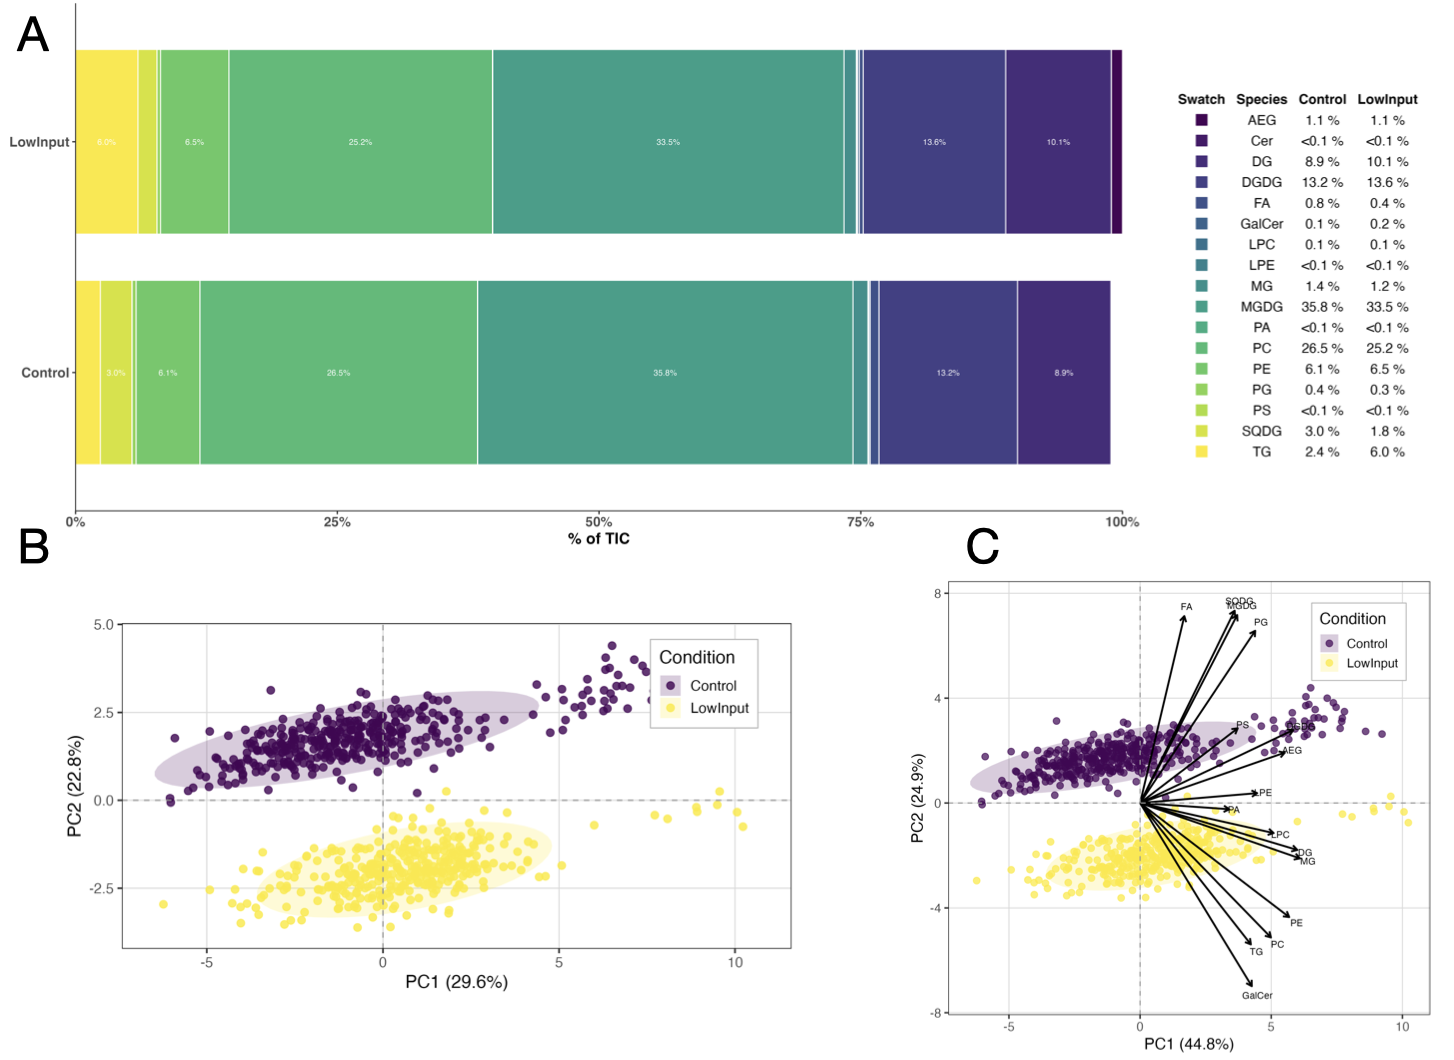
\includegraphics[width=\textwidth]{fig/main/Fig1.png}

    \caption{Overview of lipidomics for Control and Lowinput \\
    \textbf{(A)} Percent‐of‐TIC breakdown for individual lipid \emph{species}, averaged across all C (n = 384) and LI (n = 362) samples. Only species whose mean contribution >= 3 \% are labeled in‐bar.  
    \textbf{(B)} PCA biplot of individual lipid species, with scores colored by condition and vectors showing species loadings. Each point represents a sample, projected based on the log-transformed relative abundance of all individual lipid molecules. Samples from the Control condition (purple) cluster in the upper-right quadrant, while those from the LowInput condition (yellow) shift toward the lower-left, indicating broad reprogramming of lipid composition under stress. The separation along PC1 (29.6\%) and PC2 (22.8\%) captures variance driven by both lipid abundance and diversity at the species level.
    \textbf{(C)} PCA biplot of summed lipid classes, with sample scores and class‐ratio loadings.}
    
  \label{fig:Fig1_lipid_class}
\end{figure}

\subsection*{Lipid remodeling revealed by PCA and OPLS-DA}

Fig \ref{fig:Fig2:OPLS} Panel A presents a PCA of the individual lipid species, where each point represents a sample. The initial two components elucidate approximately 58.5\% of the total variance, with PC1 contributing 38.3\% and PC2 contributing 20.2\%. Samples are distinctly resolved according to condition along PC1. LowInput (LI) scores are displaced towards positive PC1 values and coalesce into a compact cluster, whereas Control (C) scores are located at negative PC1 values with no overlap. PC2 encapsulates secondary structure in the data, as C samples depict an oblique band extending from positive to negative PC2, indicative of coordinated covariation among subsets of lipids, while LI samples remain narrowly concentrated near PC2 $\approx$ 0 with limited dispersion. As separation occurs along the variance-maximizing axis, the figure suggests a comprehensive, multivariate reorganization of the lipidome rather than an influence exerted by a limited number of outliers. Hence, Fig \ref{fig:Fig2:OPLS} Panel A demonstrates that the condition alone accounts for the majority of between-sample variance in the species-level data, and that LI engenders a more homogenous lipid state compared to C.

Fig \ref{fig:Fig2:OPLS} Panel B provides a summary of a PCA conducted on class level summed glycerolipids and glycerophospholipids, with the loading vectors superimposed as a biplot. Collectively, PC1 (43.7\%) and PC2 (34.3\%) account for approximately 78\% of the variance, effectively distinguishing the two conditions as well. Samples obtained under the LI condition are positioned to the right (positive PC1) and slightly upward, while C samples are situated in the left–down quadrant. The arrows denote the lipid classes that drive the observed separation. Vectors oriented to the right/upward—specifically TG, MG, PE, PG, PC, and PS exhibit positive PC1 loadings, with PS, PE, MG, and TG also displaying positive PC2 loadings. Their orientation suggests that relative enrichment of these classes shifts samples towards the LI aggregation. This observation is consistent with individual class accounting that shows neutral/storage lipids (TG, MG) increase under LI, and the primary zwitterionic bilayer lipids (PC, PE, PG) are either maintained or slightly elevated (Fig \ref{fig:Fig1_lipid_class}B; Supplementary Figure \ref{fig:S5}B;Supplementary Figure \ref{fig:S5}C). Conversely, vectors oriented downwards, particularly PA and SQDG (near-vertical, negative PC2) and the galactolipids MGDG/DGDG along with DG/LPC in the lower-right quadrant represent features that situate C samples in the left–down region of the plane. Most notably, SQDG (strongly negative PC2, $\mathrm{PC1} \approx 0$) and MGDG (negative PC2 with a modest +PC1 component) carry two of the longest loadings, indicating that chloroplast glycolipid variation forms the principal axis orthogonal to the LI–C separation. Functionally, PC1 encapsulates the remodeling from a galactolipid/anionic-inclined configuration towards a storage-enhanced, zwitterionic bilayer state, whereas PC2 differentiates chloroplast signatures (MGDG/DGDG, SQDG/PA) from PC/PE/TG. The tight ellipses and minimal overlap indicate that these class-level transformations are coordinated across samples rather than being driven by outliers as well. Hence, the biplot demonstrates that the transition to LI is elucidated by synergistic elevations in TG/MG and the PC/PE/PG axis, alongside a reduction in MGDG/SQDG/PA contributions, precisely mirroring the pattern observed in the total ion current (TIC) and subclass analyses.


We also examined within-plant lipid class ratios instead of absolute abundances to elucidate the comparison of C and LI across a multi-year, multi-field design. By aggregating molecular species into their parent classes and constructing all pairwise class ratios, we effectively minimized both batch noise and field variability while preserving the biochemical contrasts indicative of membrane remodeling. Subsequently, we applied an OPLS-DA model to this matrix of ratios to pinpoint the combinations of classes that most effectively differentiate the two conditions. The scores plot ($t_1$ vs.\ $o_1$) revealed a distinct and reproducible separation of C and LI along the primary predictive axis $t_1$, which accounted for 60.9\% of the X variance in our data, with the remaining variation captured orthogonally on $o_1$ (Fig \ref{fig:Fig2:OPLS} Panel C). The model exhibited exemplary performance metrics with $R^2$Y $\approx$ 0.98 and $Q^2$ $\approx$ 0.98, signifying outstanding goodness-of-fit and predictive capacity, respectively. To prevent overfitting, 500 response-label permutations were executed. The permuted $R^2$Y and $Q^2$ values were centered close to zero with limited dispersion, whereas the observed statistics were positioned at the extreme right of their null distribution tails (exact permutation p($R^2$Y)=0.002, p($Q^2$)=0.005) Supplementary Figure \ref{fig:S6}. These evaluations support a stable, generalizable separation attributable to biological factors rather than stochastic structures within the data. For model interpretation, we ranked all ratios using variable importance (VIP) and retained those with VIP values exceeding 1 (Fig \ref{fig:Fig2:OPLS} Panel D, left). Two prominent features emerged. Firstly, ratios contrasting neutral glycerolipids with membrane classes—for instance, TG- or DG-to-phospholipid and to galactolipid ratios—exhibited high VIP values, reflecting the expansion of neutral lipids noted in the TIC summaries. Secondly, ratios within the phospholipid framework (e.g., PC/PS, PE/PS, PG/PS) scored highly, indicating a synchronized rebalancing among headgroup families rather than a comprehensive increase or decrease in total phospholipids. For each VIP-selected ratio, we presented the paired distributions by lipid class collectively (Fig \ref{fig:Fig2:OPLS} Panel D, right). These box/violin plots demonstrated that the multivariate separation was underpinned by consistent, directionally coherent univariate shifts as well as by isolated outliers. The ratios were categorized into sulfolipid, galactolipid, phospholipid, glycerolipid turnover, lysophospholipid, and others based on biological context. 

\textbf{Sulfolipid ratios}  \\
Within the sulfolipid framework, the ratio of phospho- or galactolipid to SQDG is uniformly elevated under LI conditions, while the inverse ratio of SQDG to TG is diminished in LI, compared to that observed in C conditions. Most markedly, the ratios PS/SQDG, PG/SQDG, PE/SQDG, and PC/SQDG all exhibit an upward shift in LI, and DGDG/SQDG likewise demonstrates an increase, suggesting a targeted reduction of SQDG relative to both phospholipids and DGDG in LI. Conversely, the SQDG/TG ratio decreases in LI, signifying an increase in neutral storage lipids (TG) relative to SQDG. Collectively, these trends indicate that the multivariate distinction is underpinned by a systematic shift away from chloroplast sulfolipid towards both phospholipid headgroups and neutral lipid stores. The accompanying Z-score box plots substantiate these findings. The directional shifts are consistent across samples and are not attributable to isolated outliers, thereby suggesting an authentic remodeling process as opposed to random variation.

\textbf{Galactolipid ratios}  \\
The ratios of galactolipids relative to other classes are skewed towards the C condition. Specifically, the ratios MGDG/PS, DGDG/MG, MGDG/PG, MGDG/PE, and MGDG/PC are all elevated in the C, suggesting that MGDG, and to a lesser degree DGDG, are relatively depleted under LI conditions when normalized to phospho- and monoglycerides. Conversely, two internal measurements reveal an opposite trend. MG/MGDG and DGDG/MGDG ratios are elevated under LI. This observation aligns with an increased turnover of MGDG (i.e., more MG per MGDG) and indicates a shift from MGDG to DGDG within the chloroplast galactolipid pool. Taken together, these findings suggest galactolipid remodeling in response to LI rather than a uniform gain or loss.

\textbf{Phospholipid ratios}  \\
The observed elevation in PS-denominated ratios (namely PC/PS, PE/PS, PG/PS, PA/PS) within the control group indicates a relative increase in PS levels in LI, or alternatively, a selective reduction of PC, PE, PG, and PA in comparison to PS. This phenomenon suggests a redistribution of headgroup composition favoring PS under LI conditions, rather than an overarching alteration in total phospholipid content.

\textbf{Diacylglycerol / glycerolipid turnover ratios.}
The analysis reveals that every DG-anchored metric (DG/MG, DG/TG, DG/PG, DG/PE), along with PA/TG, is higher in C, indicating that LI depletes DG (and PA) relative to both storage (TG) and membrane lipids. Mechanistically, this is consistent with DG being drawn into membrane rebuilding via the Kennedy pathway (DG + CDP--choline/ethanolamine $\rightarrow$ PC/PE) and with acyl editing (Lands' cycle) on PC/PE, where rapid deacylation--reacylation turns over acyl chains. Increased phospholipid cycling together with PC$\leftrightarrow$DG interconversion can therefore lower free DG relative to TG and membrane classes under LI.

\textbf{Lyso-phospholipid ratios}  \\
The majority of LPC‐anchored ratios, namely LPC/MG, LPC/PS, LPC/LPE, LPC/PE, LPC/PG, are elevated in the C condition indicating that there is a selective reduction of LPC under LI rather than effects related to the denominators. Mechanistically, this phenomenon aligns with a reduction in PC deacylation ($PLA_1$/$PLA_2$ activity) and/or enhanced LPC to PC reacylation (LPCAT) in LI, both of which would result in the suppression of the free LPC pool. Conversely, LPE/MGDG demonstrates an increase under LI, signifying a relative augmentation of LPE (via LPEAT-mediated acyl editing on PE) and/or a decrease in MGDG. This reflects a modest transition in the lysophospholipid balance from choline (LPC) towards ethanolamine (LPE) with interactions with plastid lipids. In summary, the observed reduction in LPC and the shift towards LPE support accelerated acyl editing on PE relative to PC under LI, without inferring substantial alterations in the overall phospholipid content.

\textbf{Other ratios}  \\
The remaining VIP\textgreater1 ratios encompass a range of categories not biologically relevant or straightforward. They predominantly reflect the two aforementioned themes. Firstly, the expansion of neutral lipids as opposed to plastid lipids, and secondly, the rebalancing centered on PS within phospholipids. The corresponding right-panel Z-scores exhibit consistent directional shifts across samples, substantiating that the OPLS-DA differentiation is upheld by coherent univariate impacts rather than anomalies.

In conclusion, the ratio-based OPLS-DA reinforces and elucidates the class-level narrative: LI samples are distinguished by a systematic redistribution towards neutral storage lipids and reallocation of specific phospholipid headgroups, whereas Control samples exhibit a membrane architecture more biased towards phosphocholine and polyunsaturated fatty acids (PUFAs). The robust cross-validated performance and rigorous permutation tests suggest that these patterns are resistant to environmental noise and represent conserved lipid remodeling rather than artifacts of the analysis process.



\begin{figure}[htbp]
  \centering
  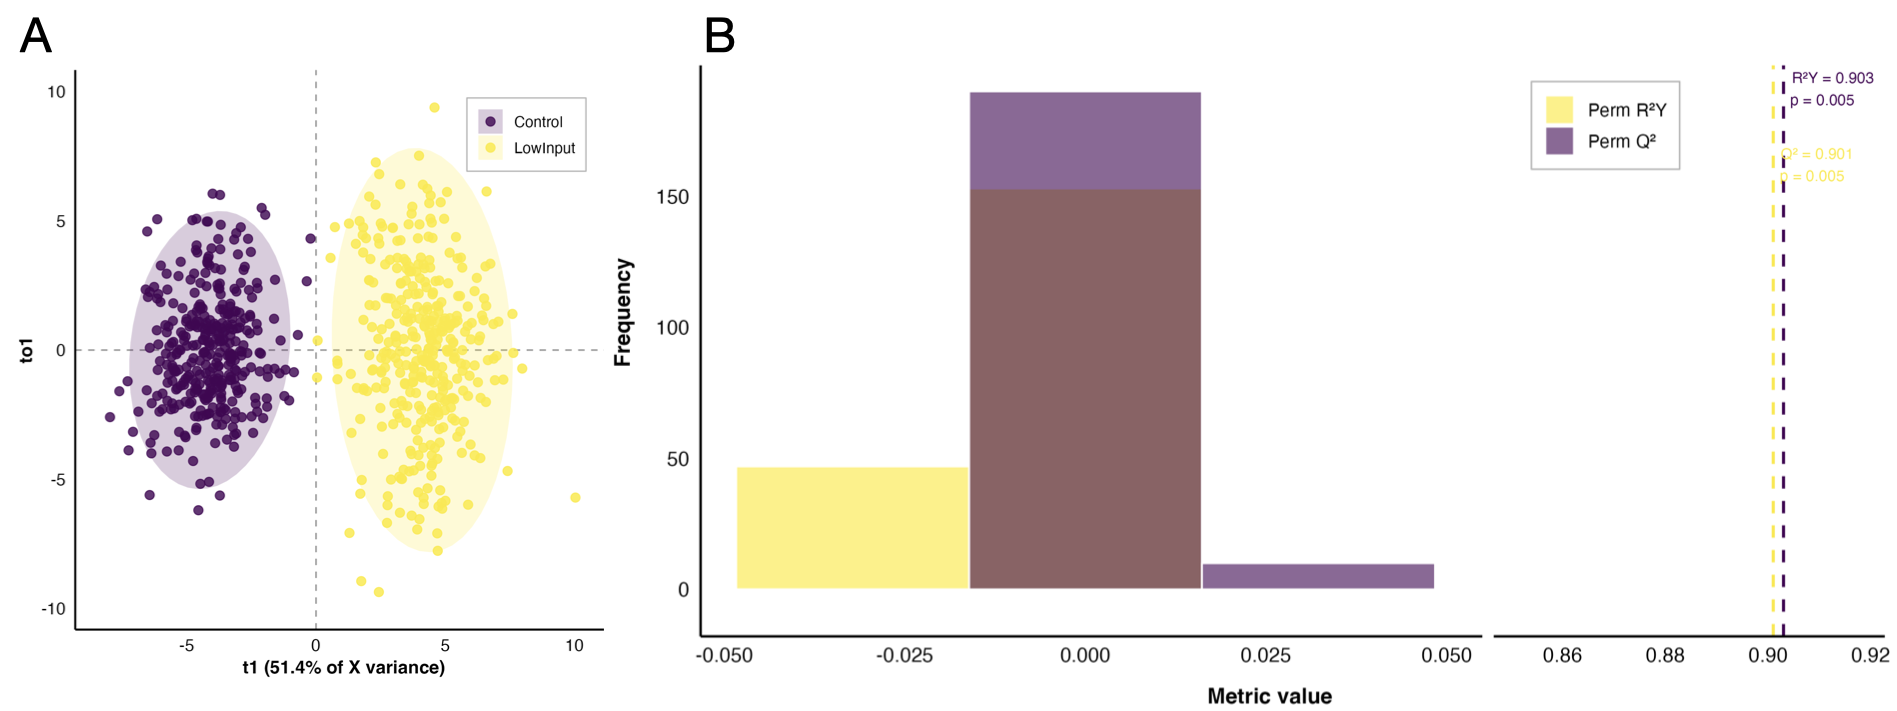
\includegraphics[width=\textwidth]{fig/main/Fig2.png}
  \caption{Orthogonal projections to latent structures discriminant analysis (OPLS‐DA) results.  
    \textbf{(A)} Score plot showing Control (purple) vs LowInput (yellow) samples on the predictive component $t_1$ (51.4\% of $X$‐variance) versus the orthogonal component $\mathrm{to}_1$, with 95\% confidence ellipses and dashed axes at zero.  
    \textbf{(B)} Permutation test: overlaid histograms of 200 permuted R²Y (yellow) and Q² (purple) values, with the true‐model metrics indicated by dashed lines (both $p=0.005$), and an arrow marking the cumulative $X$‐variance explained (R²X = 0.514).}
  \label{fig:Fig2:OPLS}
\end{figure}

\subsection*{Genome-wide Association Studies of Lipids Associated with Control and Lowinput}
We conducted GWAS with three distinct layers of data: (1) individual lipid species, which comprise both lipids  as well as other compounds (Supp Table 1), (2) aggregates of lipid class abundances, and (3) all conceivable pairwise ratios of these aggregated classes. Utilizing a significance threshold of $\log_{10}(p)\ge7$ for individual lipids and $\log_{10}(p)\ge5$ for sums and ratios , we identified W genes associated with lipid species (see Supplementary Table 2), X genes associated with other compounds (refer to Supplementary Table 3), Y genes associated with all of the summed lipid classes, and Z genes associated with the ratios of summed classes (refer to Supplementary Table 4) in a 25kb window. We conducted manual annotations for these candidate genes predicated on well-documented functions—such as lipid metabolism, N assimilation, P homeostasis, or response to cold stress. The full set of annotations is available in Supplementary Table 6. All the GWAS results can be obtained from the shiny app. Here, the candidate genes can be identified and explained using individual GWAS that gives the same candidate gene, individual GWAS relating to a particular trait, and ratio GWAS that explains some mechanisms or biological process Fig \ref{fig:Fig3}


%Re rin gwas:
%PG(16:0/18:0)

\subsection*{Phospholipid GWAS Identifies a Phosphate Starvation Response Gene}
Candidate genes were prioritized by analyzing GWAS results within the phospholipid lipid class. Notably, the Myb-like DNA-binding domain gene \texttt{SORBI\_3001G384300} was consistently identified. This gene exhibits homology with \textit{PHR1} (PHOSPHATE STARVATION RESPONSE 1) in rice, a principal regulator of phosphate homeostasis. It demonstrated associations with several phospholipid traits, namely PC(16:0/20:3), PC(16:0/22:5), PC(16:0/22:6), PC(18:1/20:1), PE(16:0/18:1), PC(18:1/24:1), PC(18:2/20:0), and PC(18:3/0:0), indicating a prospective correlation between phospholipid remodeling and phosphate starvation signaling.

\textit{PHR1} serves as a central transcription factor within plants, balancing the responses to phosphate (Pi) deprivation. It is categorized under the MYB-CC family of transcription factors and demonstrates a high level of conservation across both vascular plants and unicellular algae (Rubio et al., 2001). \textbf{PHR1} exhibits specific binding affinity to a cis-regulatory element termed the P1BS (GNATATNC) motif, which resides in the promoters of numerous genes induced by Pi starvation, thereby facilitating their expression in conditions of Pi deficiency. These genes encompass those that encode phosphate transporters, signaling components, and enzymes that partake in metabolic adaptations to Pi scarcity (Bustos et al., 2010). Loss-of-function phr1 mutants display compromised expression of genes responsive to Pi starvation and a diminished accumulation of anthocyanins, starch, and sugars under conditions of Pi deficiency, along with modified Pi distribution between roots and shoots (Rubio et al., 2001; Bustos et al., 2010). In contrast, overexpression of PHR1 results in augmented Pi uptake and improved responses to Pi starvation (Nilsson et al., 2007). In addition to maintaining phosphorus homeostasis, PHR1 also plays a crucial role in regulating sulfate homeostasis, particularly under conditions of phosphate deficiency. It enhances the expression of the sulfate transporter gene SULTR1;3 and influences the translocation of sulfate from the aerial parts to the roots during phosphorus starvation. The observation that mutants in either phr1 or sultr1;3 demonstrate diminished sulfate transfer from shoots to roots suggests that PHR1 is integral to the interaction and coordinated regulation of P and sulfur homeostasis (Rouached et al., 2011). 
%SPX1 is a nuclear protein that interacts directly with PHR1 and functions as a phosphate-dependent inhibitor of PHR1 activity. This interaction is critically influenced by intracellular phosphate (Pi) concentrations; during conditions of Pi sufficiency, SPX1 binds to PHR1, thereby inhibiting its interaction with the P1BS motif in target gene promoters and consequently repressing Pi starvation responses. Conversely, under conditions of Pi deprivation, this interaction is attenuated, allowing PHR1 to activate its target genes (Puga et al., 2014). This mechanism establishes a molecular connection between Pi sensing and signaling, wherein Pi itself regulates the activity of the PHR1 transcription factor through SPX1. Notably, the Pi analog phosphite (Phi), which lacks metabolic capability but suppresses Pi starvation responses, can replicate Pi in promoting the SPX1-PHR1 interaction, further substantiating the hypothesis that SPX1 facilitates a direct perception of Pi levels (Puga et al., 2014).



%References

%Rubio V, Linhares F, Solano R, Martín AC, Iglesias J, Leyva A, Paz-Ares J. (2001). A conserved MYB transcription factor involved in phosphate starvation signaling both in vascular plants and in unicellular algae. Genes & Development, 15(16), 2122–2133.

%Bustos R, Castrillo G, Linhares F, Puga MI, Rubio V, Pérez-Pérez J, Solano R, Leyva A, Paz-Ares J. (2010). A central regulatory system largely controls transcriptional activation and repression responses to phosphate starvation in Arabidopsis. PLoS Genetics, 6(9), e1001102.

%Nilsson L, Muller R, Nielsen TH. (2007). Increased expression of the MYB-related transcription factor, PHR1, leads to enhanced phosphate uptake in Arabidopsis thaliana. Plant Cell and Environment, 30(11), 1499–1512.

%Rouached H, Secco D, Arpat AB, Poirier Y. (2011). The transcription factor PHR1 plays a key role in the regulation of sulfate shoot-to-root flux upon phosphate starvation in Arabidopsis. BMC Plant Biology, 11, 19.

%Puga MI, Mateos I, Charukesi R, Wang Z, Franco-Zorrilla JM, de Lorenzo L, Irigoyen ML, Masiero S, Bustos R, Rodríguez J, Leyva A, Rubio V, Sommer H, Paz-Ares J. (2014). SPX1 is a phosphate-dependent inhibitor of PHOSPHATE STARVATION RESPONSE 1 in Arabidopsis. Proceedings of the National Academy of Sciences of the United States of America, 111(41), 14947–14952.



\subsection*{DGAT1 Controls Triacylglycerol Storage in Response to Nitrogen Limitation and Cold}

We identified the gene \textit{SORBI\_3010G170000}, which encodes Acyl‐CoA:diacylglycerol acyltransferase 1 (DGAT1, analogous to Arabidopsis TG1), in five distinct GWASs: TG(18:1/18:3/22:0), TG(518:2/20:3/22:0), TG(18:2/18:2/18:4), TG(18:2/20:3/22:0), and TG(18:3/18:3/18:3). DGAT1 is responsible for the essential final conversion of DG into TG, which is a key lipid for carbon and energy storage in seeds and stress-affected vegetative tissues \cite{Zhang2009,Yang2011}. In Arabidopsis, low N levels result in the TG accumulation within leaves due to increased levels of DGAT1 and OLEOSIN1 \cite{Yang2011}. The ABA signaling pathway, involving the transcription factor ABI4, directly stimulates DGAT1 by interacting with CE1 elements (CACCG) in its promoter. In \emph{abi4} mutants, both DGAT1 stimulation and TG accumulation are reduced, emphasizing the significance of ABI4 during N deficiency \cite{Yang2011}. Additionally, DGAT1 is highly responsive to cold temperatures (4°C) and plays an essential role in freeze tolerance. Arabidopsis mutants deficient in \emph{dgat1} develop chlorosis and increased cell mortality under cold stress, with reduced TG but higher DG and PA levels \cite{Tan2018}. This elevated PA production induces RbohD-dependent ROS formation, causing oxidative stress. Increased DG kinase activity (DGK2/3/5) (GWAS results) further boosts PA, while the removal of \emph{dgk} genes restores cold tolerance, suggesting a balance between DGAT1 and DGK is essential for managing ROS and adapting to cold stress \cite{Tan2018}. In seeds, both DGAT1 and phospholipid:diacylglycerol acyltransferase 1 (PDAT1) are vital for optimal oil body development. \emph{dgat1} mutants have a 20–40\% decline in seed oil content (see Lipid annotation Section 5), whereas double mutants (\emph{dgat1/pdat1}) or RNAi lines demonstrate an 80\% decrease in TG, resulting in fertility and embryonic issues \cite{Zhang2009}. Overexpression of DGAT1 enhances seed weight and oil production, highlighting its crucial role in regulating TG levels throughout plant development \cite{Zhang2009,Yang2011}.



\subsection*{Sum of SQDG GWAS Identifies a Sulphate Assimilation Gene}
Our GWAS for the sum of SQDG identified a sulphate assimilation gene, called the adenylyl-sulfate kinase gene (APK3). APK3 is one of the four isoforms of APS kinase (adenosine 5'-phosphosulfate kinase) in Arabidopsis thaliana, an enzyme that plays a critical role in sulfur metabolism by phosphorylating adenosine 5'-phosphosulfate (APS) to produce 3'-phosphoadenosine 5'-phosphosulfate (PAPS), the active sulfate donor required for sulfation reactions in secondary metabolism (Mugford et al., 2009, p.1-2). Unlike the other APK isoforms, APK3 is uniquely localized in the cytosol, whereas APK1, APK2, and APK4 are plastid-localized (Mugford et al., 2009, p.4). The enzyme's activity influences sulfur partitioning between primary and secondary metabolism, particularly affecting the synthesis of sulfated secondary metabolites such as glucosinolates, which are important for plant defense (Mugford et al., 2009, p.1-2). Studies have shown that disruption of APK1 and APK2 leads to a significant reduction in glucosinolate levels and an increase in thiols, indicating that APKs regulate the availability of PAPS and thus control the flux toward secondary sulfated compounds (Mugford et al., 2009, p.2-3). However, the specific disruption of APK3, the cytosolic isoform, does not significantly affect primary sulfate assimilation or glucosinolate levels, suggesting a more specialized or possibly redundant role compared to plastidic APKs (Mugford et al., 2009, p.4). Furthermore, the C-terminal STAS domain of SULTR1;2, a sulfate transporter, interacts with OAS-TL and is involved in feedback regulation of sulfate transporter activity, but how APK3 activity integrates within this regulatory network remains unclear (Sum\_SQDG\_APK3\_S\_starvation.pdf, p.4). Overall, APK3 contributes to sulfur metabolism by modulating PAPS production in the cytosol, influencing sulfur flux balancing, but its precise regulatory role requires further elucidation.

%References:

%Mugford, S.G., Lee, B.-R., Koprivova, A., Matthewman, C.A., and Kopriva, S. (2009). Disruption of adenosine-5′-phosphosulfate kinase in Arabidopsis reduces levels of sulfated secondary metabolites. Plant Cell 21, 910–927. (Sum_SQDG_APK3_secondary_S.pdf, pp. 1–5)
%Kopriva, S., Mugford, S.G., Baraniecka, P., Lee, B.R., Matthewman, C.A., and Koprivova, A. (2012). Control of sulfur partitioning between primary and secondary metabolism in Arabidopsis. Frontiers in Plant Science, 3, 163. (Sum_SQDG_APK3_S_starvation.pdf, p.14)
%Takahashi, H. (2019). Sulfate transport systems in plants: functional diversity and molecular mechanisms underlying regulatory coordination. J. Exp. Bot. 70, 4075–4087. (Sum_SQDG_APK3_S_starvation.pdf, p.16) 


%\subsection*{SQDG Metabolism and Its Role in Phosphate‐Starvation Responses}

%In our GWAS of SQDG(32:0) levels, the top locus was \textit{SORBI\_3002G000600}, which encodes the plant ortholog of sulfoquinovosyltransferase (SQD2). SQDG is a negatively charged glycolipid (sulfoquinovose = 6‑deoxy‑6‑sulfonato‑glucose) that constitutes up to 10–20\% of chloroplast thylakoid lipids and is critical for stabilizing photosystem II, photosystem I, and cytochrome \emph{b}\(_6\)\emph{f} complexes \citep{Yu2002,Qin2015,Umena2011}.

%Biosynthesis proceeds in two enzymatic steps \citep{Yu2002,Sun2021}:
%\begin{enumerate}[label=(\arabic*)]
%  \item \textit{SQD1} (UDP‑sulfoquinovose synthase): 
%        \[
%           \mathrm{UDP\!-\!Glc} + \mathrm{SO_3^{2-}} \;\longrightarrow\; \mathrm{UDP\!-\!sulfoquinovose}
%        \]
%  \item \textit{SQD2} (sulfoquinovosyltransferase): 
%        \[
%           \mathrm{UDP\!-\!sulfoquinovose} + %\mathrm{diacylglycerol} \;\longrightarrow\; \mathrm{SQDG}
%        \]
%\end{enumerate}

%Under phosphate (Pi) starvation, plants degrade phospholipids (e.g.\ PG) to recycle Pi, while \textit{SQD1} and \textit{SQD2} are transcriptionally upregulated, leading to increased SQDG accumulation and preservation of thylakoid membrane functions \citep{Essigmann1998,Nakamura2013,Sun2021}. In rice, \textit{OsPHR2} directly activates \textit{OsSQD1} under Pi deficiency, and loss of \textit{OsPHR2} impairs SQDG levels, alters fatty‐acid composition, and reduces photosynthetic efficiency \citep{Sun2021}. Similarly, \emph{sqd2} mutants in \emph{Arabidopsis thaliana} are unable to synthesize SQDG and exhibit growth defects under low‐Pi conditions, underscoring the essential role of SQDG in replacing anionic phospholipids in the chloroplast \citep{Yu2002}.


%\subsection*{Senescence‐linked lipid remodeling and the SAG39 candidate}

%Tier 1 – strongest mechanistic readouts (use these first)
%Sum_LPE / Sum_MGDG and Sum_LPC / Sum_MGDG
%Lysophospholipids (LPE/LPC) rise with PLA-mediated deacylation during membrane breakdown, while MGDG (core thylakoid galactolipid) falls as chloroplasts dismantle. These ratios jump when senescence intensifies—exactly the context where a SAD39 protease would be high.

%Sum_DGDG / Sum_PS and Sum_PG / Sum_PS
%DGDG/PG are plastid lipids; PS is extraplastidic/ER-derived. Senescence shifts lipid balance away from plastid membranes and toward extraplastidic pools. Expect these ratios to decrease with stronger senescence.

%Tier 2 – flux to storage / membrane remodeling (very good)
%Sum_DG / Sum_TG
%Senescing leaves divert DAG to TAG (lipid droplets). As storage rises, DG/TG tends to drop. A SAD39 allele marking stronger senescence should track that direction.
%Sum_PC / Sum_SQDG and Sum_PE / Sum_SQDG
%SQDG (plastid sulfolipid) diminishes with thylakoid loss; PC/PE (ER phospholipids) often hold or increase. These ratios typically increase with senescence.

%Our GWAS identified a senescence-specific cysteine protease SORBI\_3010G113600 (SAG39) as a candidate based on distinctive membrane lipid ratios (Supplementary Table), particularly LPE/MGDG and plastid/extraplastid contrasts such as DGDG/PS and PG/PS. These lipid ratios are mechanistically involved in chloroplast dismantling, a defining feature of senescence. Under low-input conditions, there is a decline in chloroplast thylakoid galactolipids like MGDG and DGDG (Fig), attributed to PLA-type deacylation. Conversely, lysophospholipids such as LPE and LPC accumulate as direct products of phospholipase activity (Jimbo \& Wada, 2023; Domínguez \& Cejudo, 2021). Therefore, the rise in LPE/MGDG suggests an active deacylation process of chloroplast membranes, leading to a reduction in thylakoid mass. This creates a biochemical environment where proteases such as SAG39 are involved in breaking down stromal and thylakoid proteins (Fig).

%Similarly, during leaf senescence, the ratio of DGDG to PS declines, signifying a redistribution of lipid pools from plastid-dominated galactolipids to extraplastidial phospholipids. DGDG is a crucial component of thylakoid membranes, responsible for maintaining the structure and stability of photosynthetic complexes. However, it undergoes active degradation during chloroplast dismantling, a pivotal event in senescence, mediated through the activity of galactosidases and lipases that liberate its constituent diacylglycerol and galactose (Domínguez \& Cejudo, 2021; Lee et al., 2009; Springer et al., 2016). This depletion of plastidial galactolipids causes a reduction in the numerator of the DGDG/PS ratio. In contrast, PS, an extraplastidial phospholipid primarily situated in the inner leaflet of the plasma membrane and endomembrane system, undergoes dynamic remodeling during senescence, specifically through the elongation of its acyl chains from approximately C37 to C41 (Li et al., 2014). This elongation is accelerated under conditions of stress and aging, potentially stabilizing membrane curvature or aiding in repair, whereas excessive elongation and eventual externalization of PS can also signal programmed cell death. As plastid membranes disassemble and extraplastidial membranes undergo remodeling, the relative abundance of PS increases (Supp Fig 5), contributing to the reduction in the DGDG/PS ratio. Consequently, a decreasing DGDG/PS ratio encapsulates both aspects of senescence-associated membrane remodeling: the enzymatic degradation of plastid galactolipids and the compositional and structural modifications within extraplastidial PS. This ratio serves as a reliable biochemical marker that signifies the transition from plastid lipid pools to extraplastid lipid pools, supporting nutrient recycling, membrane restructuring, and cellular reprogramming during leaf senescence (Domínguez \& Cejudo, 2021; Li et al., 2014).

%Thus, the presence of SAG39 in these ratio GWAS strengthens the interpretation that our low‐input lipidomic shifts are not incidental but part of a coordinated senescence program coupling lipid catabolism, proteolysis, and neutral‐lipid sequestration (Besagni \& Kessler, 2013; Wang et al., 2018; Domínguez & Cejudo, 2021; Jimbo & Wada, 2023).


%\subsection*{MG and MGDG Ratio GWAS Identifies a PG Biosynthesis Gene}
%Among the three stressors, anticipated lipid alterations establish a flux competition at the DAG/CDP-DAG hub, potentially driving MG/MGDG downward while rendering genotypic differences in PG synthesis highly significant. Under conditions of nitrogen deficiency, the biogenesis of thylakoid membranes decelerates, leading to a reduction in chlorophyll content, impairment of chloroplast ultrastructure, and a decrease in MGDG levels, particularly in highly unsaturated forms such as 34:6- and 36:6-MGDG, along with other thylakoid lipids. This results in a decline of the MG/MGDG ratio due to a diminishing denominator (MGDG), with MG often also experiencing a decline as a consequence of reduced thylakoid membrane construction or turnover. Phosphorus deficiency typically induces a substitution of phospholipids by galactolipids, resulting in PG depletion and an increase in non-phosphorus lipids such as MGDG/DGDG and SQDG. Nevertheless, this lipid remodeling relies on the same DAG/CDP-DAG precursor pool, whereby genetic variability in the metabolic pathway towards PG as opposed to galactolipids can alter the MGDG supply and thus affect the MG/MGDG ratio.

%Cold conditions specifically enhance the dependency on phosphatidylglycerol (PG) for the function of photosystems. PG plays a critical role in the structure, repair, and stability of photosystem II and I (PSII/PSI), and cold-tolerant plant species often adjust PG content and degree of unsaturation to sustain photosynthetic efficacy. The biosynthesis of plastidic PG follows a pathway from CDP-diacylglycerol (CDP-DAG) to phosphatidylglycerophosphate (PGP) to PG; mutations affecting this pathway, such as those observed in PGP1, result in photosynthetic impairments. In cold environments, plants tend to sustain or increase PG levels even under conditions of low phosphorus availability, as PG is functionally irreplaceable, with squamous glycolipid (SQDG) only capable of partially substituting for it. Cold stress also disrupts the fluxes of phosphatidylcholine (PC) and phosphatidic acid (PA) that converge at the same diacylglycerol (DAG) pool, thereby further affecting monogalactosyldiacylglycerol (MGDG) availability.

%Integrating these observed phenomena within the context of the low-input (LI) treatment reveals that reduced nitrogen levels lead to the contraction of thylakoid membranes, thereby decreasing MGDG; phosphate deficiency would typically suppress PG levels, yet low temperatures mitigate this effect by ensuring the maintenance of PG for the stabilization and repair of photosystems. Our data elucidate a net result — a decrease in MG and MGDG, and an increase (or preservation) of PG — which aligns with a cold-induced fortification of PG that overrides aspects of the low-phosphate substitution framework. This biochemical competition clarifies why allelic variations within the plastid PG-biosynthesis pathway (e.g., CDS/PGP) emerge as significant in GWAS: genotypes that channel increased DAG/CDP-DAG flux to PG consequently deplete the DAG available for MGDG, further reducing MG/MGDG levels and positioning the PG gene as the predominant association, despite PG itself not forming part of the ratio.

%Phosphatidylglycerol (PG) constitutes the primary phospholipid within chloroplasts and is integral to plant tolerance against chilling stress. It is exclusively synthesized through the prokaryotic pathway within chloroplasts, and it is essential for both the development of chloroplasts and their photosynthetic functionality (Nussberger et al., 1993; Hagio et al., 2002; Wada & Murata, 2007). The fatty acid composition of PG, particularly the proportion of high-melting-point molecular species (HMP-PG) enriched in 16:0, 18:0, and 16:1-trans, is closely associated with chilling sensitivity. Plants resistant to chilling typically possess less than 10 \% HMP-PG, whereas numerous chilling-sensitive species have levels exceeding 30 \% (Murata, 1983; Roughan, 1985; Wada & Murata, 2007). Elevated HMP-PG levels induce a gel-phase transition at reduced temperatures, thereby perturbing membrane fluidity and resulting in cellular damage (Murata & Yamaya, 1984). Genetic and transgenic investigations have substantiated that increased HMP-PG content instigates chilling sensitivity. For instance, the Arabidopsis fab1 mutant, which accumulates approximately 40–50 \% HMP-PG, experiences a collapse in photosynthesis and eventual death after prolonged exposure to cold (Wu & Browse, 1995; Barkan et al., 2006; Gao et al., 2015). The targeted reduction of HMP-PG in fab1 restores cold tolerance, thereby demonstrating causality (Gao et al., 2020). This accumulation of evidence emphasizes the role of PG biosynthesis genes as critical regulatory points under light and temperature stress. They influence the MG/MGDG ratio indirectly via precursor competition and directly determine the plant’s capacity to sustain photosynthetic proficiency and withstand combined nutrient and temperature challenges.

%References (as provided):
%Nitrogen_deficiency.pdf pp. 6–9; membrane_remodeling_phosphorus.pdf pp. 237–243; membrane_lipid_P_reuse.pdf pp. 13–14; glycerolipid_remodeling_P_starve.pdf p. 7; glycolipid_remodeling_nitrogen_phosphorus_deficiency.pdf p. 13; Cold_tolerance_barley.pdf pp. 7–9; Glycerolipid_freezing.pdf pp. 4–8; Photosynthesis_thylakoid_glycerolipid.pdf pp. 4–7; Cold_tolerance_maize.pdf pp. 8–9.
%Nussberger et al., 1993; Hagio et al., 2002; Wada & Murata, 2007; Murata, 1983; Roughan, 1985; Murata & Yamaya, 1984; Murata et al., 1992; Wolter et al., 1992; Moon et al., 1995; Ishizaki-Nishizawa et al., 1996; Wu & Browse, 1995; Barkan et al., 2006; Gao et al., 2015; Gao et al., 2020.

\subsection*{Alternative Oxidase Roles in Photoprotection and Nitrate Assimilation}

Through our GWAS focused on alpha-carotene, we  identified an alternative oxidase (AOX) gene. Alpha-carotene (\(\alpha\)-carotene), a secondary chloroplast carotenoid, is primarily located within the reaction centers of photosystem I (PSI) and photosystem II (PSII), with only minor quantities found in the peripheral light-harvesting complexes \citep{Young1989}. It bears structural similarity to \(\beta\)-carotene, absorbs blue-green light, and facilitates energy transfer to chlorophyll while concurrently quenching triplet chlorophyll and reactive oxygen species (ROS) to safeguard the photosynthetic apparatus from photooxidative damage under intense light stress. Its co-localization with \(\beta\)-carotene in pigment–protein complexes indicates a contributory role in stabilizing the core structures of PSII and PSI \citep{Young1989}. The mitochondrial AOX pathway offers a non-phosphorylating alternative to cytochrome oxidase, directly oxidizing ubiquinol to water, thereby preventing over-reduction of the photosynthetic electron transport chain \citep{Vishwakarma2015}. AOX1A, the dominant isoform in green tissues, plays a role in dissipating excess reducing equivalents produced by photosynthesis, supports non-photochemical quenching (NPQ), and collaborates with the chloroplast malate–oxaloacetate shuttle to sustain cellular redox homeostasis. Under conditions of stress, such as high light or drought, that inhibit the cytochrome pathway, AOX activity curbs ROS formation and maintains photosynthetic efficiency \citep{Vishwakarma2015}. In addition to its photoprotective function, AOX is vital for nitrate assimilation in plants. During NO\(_3^-\) reduction, the accumulation of reducing equivalents may lead to chloroplast over-reduction; AOX counters this by channeling excess reductants into mitochondrial respiration, thereby preventing oxidative stress and sustaining photosynthesis \citep{Gandin2014}. Studies involving \emph{aox1a} T-DNA insertion mutants in \emph{Arabidopsis thaliana} corroborate that AOX engages with nitrate assimilation pathways to uphold redox balance and optimize C-N metabolism under varying N conditions \citep{Gandin2014,Vishwakarma2015}.


%\subsection*{Beta‑Sitosterol GWAS Links Cellulose Synthase to Membrane Stability}
%In our GWAS of beta-sitosterol (BS), we detected a significant association peak at the cellulose synthase locus SORBI\_3003G049600, indicating that variations in this CesA gene may affect BS accumulation or its function in stabilizing membranes in sorghum. BS is a common phytosterol in plants that integrates into lipid bilayers to regulate membrane fluidity and stability. Although its exact role in cell wall structure is not fully understood, BS is suggested to protect cells from abiotic and biotic stress by enhancing plasma membrane integrity and potentially interacting with cytoplasmic and chloroplast membranes \citep{Sayeed2016}. Studies from Arabidopsis implies that BS plays a role in defense responses, yet a conclusive characterization of its role in cell wall mechanics remains necessary \citep{Sayeed2016}. The cellulose synthase (CesA) complexes are responsible for synthesizing the β-1,4-glucan chains of cellulose, the primary load-bearing polysaccharide in plant cell walls. In Arabidopsis, specific CesA isoforms form plasma-membrane rosettes to produce primary-wall (e.g., AtCesA1, 3, 6) and secondary-wall cellulose (e.g., AtCesA4, 7, 8), which support cell expansion, mechanical strength, and biomass accumulation \citep{Mueller1980,Somerville2006,Hu2018}. Mutations in CesA genes (e.g., \emph{rsw1}, \emph{prc1‑1}) result in decreased cellulose content, weakened cell walls, altered cell morphology, and reduced stress resistance \citep{Hu2018,Arioli1998,Persson2007,CanoDelgado2003,HernandezBlanco2007}. Although CesA primarily directs carbon towards cellulose production, downregulation or mutation of certain CesA genes can redirect carbon flux towards storage compounds. In Arabidopsis seeds, suppression of CesA leads to a slight reduction in cellulose content and prompts compensatory increases in non-cellulosic polysaccharides or proteins \citep{Hu2020}. It has been proposed that redirecting carbon from cell wall polysaccharides to seed storage proteins and oils may enhance nutritional quality, addressing the inverse relationship between seed oil and protein content \citep{Tomlinson2004,Ekman2008,Iyer2008,Shi2012,Tan2011,YoshieStark2008,Knowles1983}. 


\subsection*{Gibberellic Acid Response GWAS Identifies a MADS‑Box Regulator of Flowering Time}

In the gibberellic acid (GA) genome-wide association study (GWAS), we detected the \textit{SORBI\_3007G090421}. GA\(_3\) enhances floral initiation in short-day sorghum genotypes, predominantly when in conjunction with far-red light (FR). Williams and Morgan (1979) demonstrated that the combination of GA\(_3\) and FR results in an advancement of flowering by 30 to 80 days in early to intermediate maturity lines, and independently facilitates stem elongation \citep{Williams1979}. Lee \emph{et al.} (1998) further elucidated that photoperiod and phytochrome B are instrumental in regulating endogenous GA\(_1\)/GA\(_{20}\) rhythms, with altered GA peaks in \emph{phyB}-deficient genotypes being associated with early flowering under non-inductive day lengths \citep{Lee1998}. In our GA\(_3\) GWAS, the MADS-box transcription factor gene SORBI\_3007G090421 was identified. MADS-box proteins, particularly Type II C-function genes, are key regulators of floral organ identity and flowering time, whereas Type I MADS (e.g., \emph{AGL62}) affects endosperm development with consequential indirect effects on reproductive timing \citep{Paul2020}. Environmental temperature influences the effects of GA3 on development; Jabir and Mahmoud (2021) reported that elevated temperatures at planting dates, coupled with GA\(_3\) (100 ppm), expedited sorghum flowering, improved germination, and enhanced enzymatic activities for nutrient mobilization \citep{Jabir2021}. Williams and Morgan also observed genotype-specific temperature responses under controlled versus field conditions, casting light on temperature as a crucial element in GA3-mediated flowering regulation.


\subsection*{GWAS of Zeaxanthin Reveals High Light-inducible Protein}

Zeaxanthin is an essential carotenoid that plays a significant role in the photoprotection mechanisms of photosynthetic organisms, predominantly acting within the framework of the xanthophyll cycle. Under conditions of high light (HL) stress, violaxanthin undergoes enzymatic de-epoxidation to form antheraxanthin, which is further converted into zeaxanthin. This carotenoid is instrumental in dissipating excess excitation energy by quenching excited chlorophyll molecules. The process effectively averts the generation of deleterious reactive oxygen species (ROS), thus safeguarding photosystem II (PSII) from photoinhibition (Levin and Schuster 2023). Zeaxanthin associates with light-harvesting complexes, such as LHCII and certain LHC-like proteins, thereby facilitating non-photochemical quenching (NPQ) to efficiently transmute excess absorbed photonic energy into thermal energy (Levin and Schuster 2023).

Our GWAS for zeaxanthin has identified the gene SORBI\_3002G033800, which has an orthologous counterpart in Arabidopsis, referred to as One-helix proteins (OHPs). These OHPs share homology with the high light-inducible proteins (HLIPs) found in cyanobacteria. These functions as small chlorophyll a/b-binding proteins characterized by a single transmembrane helix with an LHC motif. OHPs are upregulated under high light conditions, playing a pivotal role in the biogenesis and repair of PSII. They transiently associate with PSII core proteins and temporarily bind chlorophyll pigments during the PSII repair cycle, shielding chlorophyll molecules from photooxidative damage by facilitating energy dissipation through the direct transfer between chlorophyll a and β-carotene (Levin and Schuster 2023). In Arabidopsis, mutations in OHP1 result in compromised chlorophyll accumulation, thylakoid architecture, and photosystem functionality, highlighting their essential role in photoprotection and photosynthetic efficiency (Levin and Schuster 2023).


%References:
%Levin, G., & Schuster, G. (2023). LHC-like Proteins: The Guardians of Photosynthesis. International Journal of Molecular Sciences, 24, 2503. 12568911
%Levin, G., Yasmin, M., Simanowitz, M.C., Meir, A., Tadmor, Y., Hirschberg, J., Adir, N., & Schuster, G. (2022). A Desert Green Alga That Thrives at Extreme High-Light Intensities Using a Unique Photoinhibition Protection Mechanism. bioRxiv. 911
%Myouga, F., Takahashi, K., Tanaka, R., Nagata, N., Kiss, A.Z., Funk, C., Nomura, Y., Nakagami, H., Jansson, S., and Shinozaki, K. (2018). Stable accumulation of photosystem II requires ONE-HELIX PROTEIN1 (OHP1) of the light harvesting-like family. Plant Physiology, 176(4), 2277–2291.
%Hey, D., and Grimm, B. (2018). ONE-HELIX PROTEIN2 (OHP2) is required for the stability of OHP1 and assembly factor HCF244 and is functionally linked to PSII biogenesis. Plant Physiology, 177(4), 1453–1472.

\begin{figure}[htbp]
  \centering
  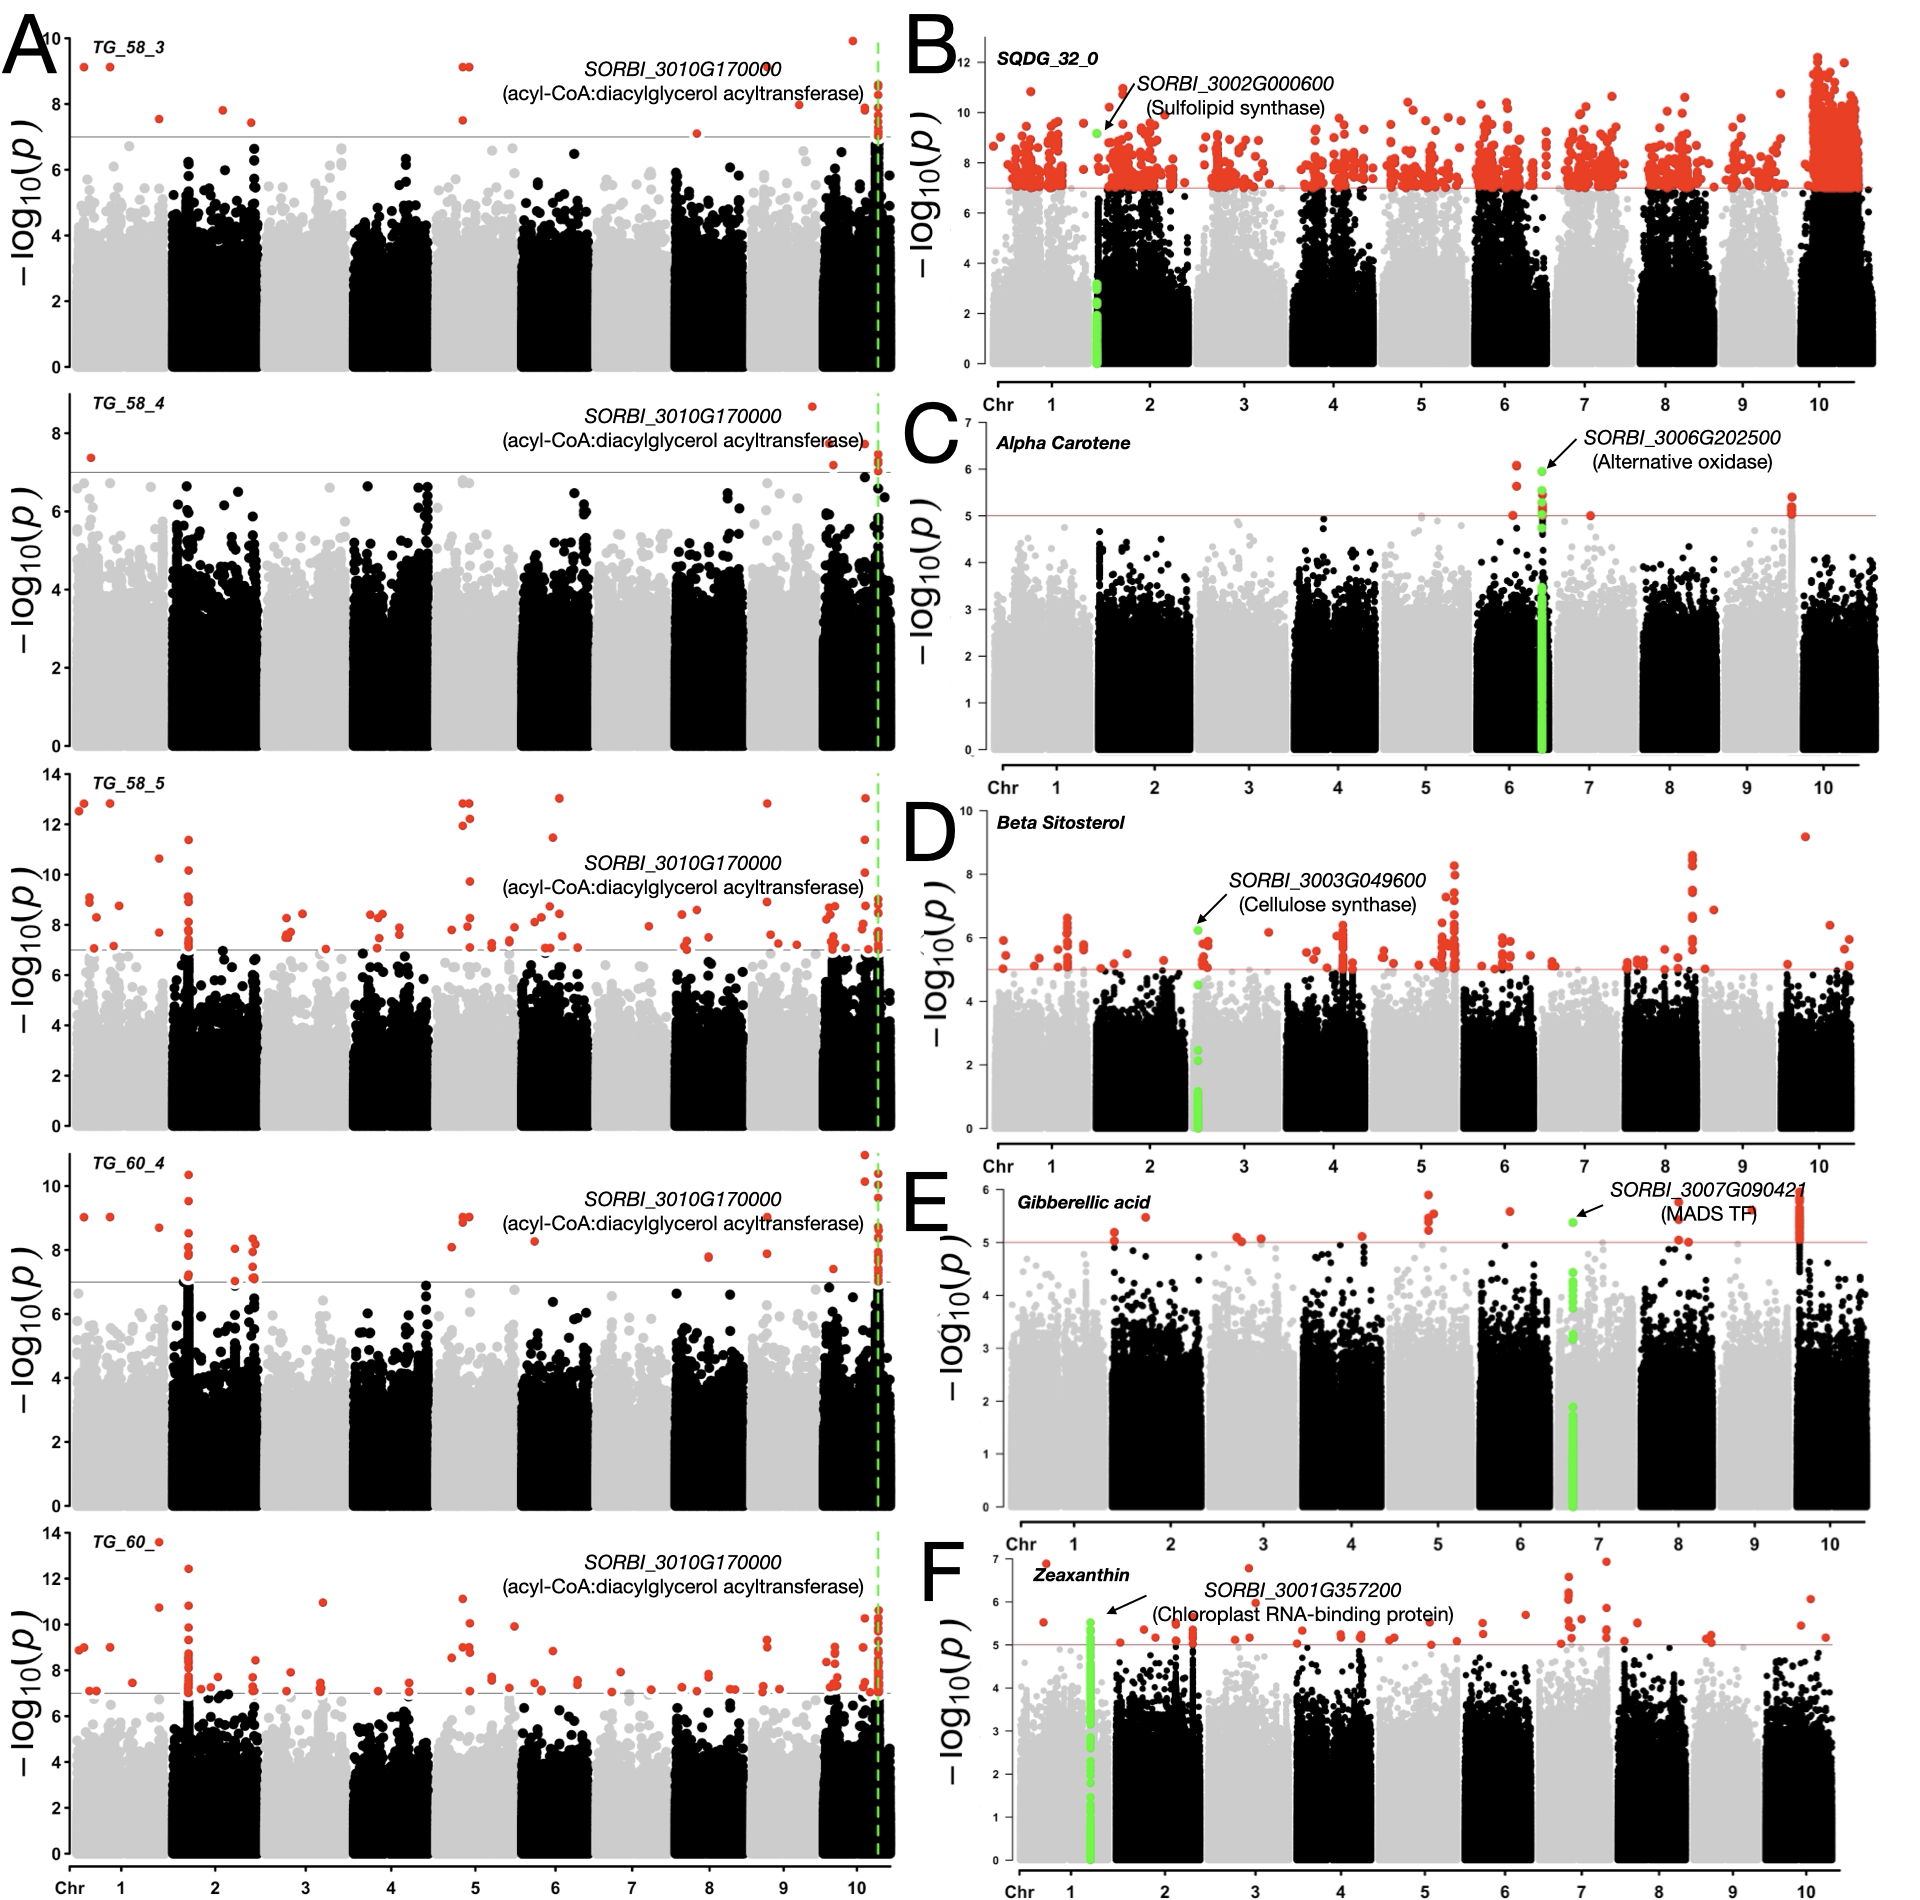
\includegraphics[width=\textwidth]{fig/main/Fig3.png}
  \caption{\textbf{Low‐input lipid GWAS Manhattan plots}
    \textbf{(A)} Manhattan plots for five Phosphplipids PC(16:0/20:3),PC(16:0/22:5),PC(16:0/22:6),PC(16:1/20:1), and PE(16:1/18:1), all peaking at PHR1 locus (\textit{SORBI\_3001G384300}) in chromosome 1; the vertical green dashed line marks the SNP position for this gene.  
    \textbf{(B)} Manhattan plots for five TG species TG(18:1/18:3/22:0),TG(18:1/20:3/22:0),PC(18:2/18:2/16:4),TG(18:2/20:3/22:0), and TG(18:3/18:3/18:3), all peaking at DGAT1 locus (\textit{SORBI\_3010G170000}) in chromosome 10; the vertical green dashed line marks the SNP position for this gene. 
    \textbf{(C)} Sum of SQDG Manhattan plot, identifying an adenylate sulfate kinase (\textit{SORBI\_3005G195600}).  
    \textbf{(D)} \(\alpha\)‐Carotene Manhattan plot, identifying an alternative oxidase (\textit{SORBI\_3006G202500}).  
    \textbf{(E)} Gibberellic acid Manhattan plot, at a sugar transporter SORBI/_3010G030600 and a MADS‐box transcription factor locus (\textit{SORBI\_3007G090421}) .  
    \textbf{(F)} Zeaxanthin Manhattan plot, marking a chloroplast RNA‐binding protein (\textit{SORBI\_3001G357200}).  
    Green dots indicate SNPs within or near the highlighted genes in panels B–F. Panels A and B show traditional lipids (–log\textsubscript{10} $p$\(\geq\)7), and panels C–F show non‐traditional lipids (–log\textsubscript{10} $p$\(\geq\)5).}
  \label{fig:Fig3}
\end{figure}


%\subsection*{Lipid Changes under LowInput (LI)}
%The multi-year, multi-field experimental design introduced considerable environmental variability into the lipidomic profiles. Although spatial corrections (SpATS) and batch-effect normalization (SERRF) were employed, residual confounding factors necessitated a ratio-based analytical approach to compare the C and the LI conditions. Lipid class ratios, which demonstrate greater resilience to technical and environmental noise than absolute abundances, were prioritized to identify biologically conserved patterns of membrane adaptation. To mitigate these confounding effects, we concentrated on within-plant lipid class ratios, expected to be fairly consistent under a variety of cultivation environments, rather than absolute abundances. We aggregated individual molecular species into their respective lipid classes, computed all possible pairwise ratios on a linear scale, and subsequently applied OPLS-DA to identify the most discriminative ratios. The resulting scores plot (Fig. \ref{fig:Fig2:OPLS}) demonstrated a robust separation of C versus LI samples, and the model exhibited exemplary performance metrics (R²Y = 0.99; Q²Y = 0.82) alongside a highly significant CV-ANOVA (p \textless 0.001) (Supp Figure, supp table). Hotelling’s T² analysis confirmed the absence of extreme outliers, and a 1,000-permutation test dismissed overfitting, indicating that our observations are unlikely attributable to chance. From the complete ratio set, 21 features surpassed a conservative VIP threshold of 1. Each of these high VIP ratios was then subjected to univariate testing (adjusted p \textle 0.05) and cross-verified against established pathways of membrane remodeling under cold and nutrient stress. The two-tier selection approach prioritizing statistical power and biological relevance yielded a defined set of lipid-class ratios (supp table) which may differentiate between C and LI. These lipid ratios are used for the further studying the effects of C and LI. 





%SORBI_3006G214500 - Lecithin cholesterol acyltransferase like 4
%SORBI_3001G448800 - Lecithin cholesterol acyltransferase like 1
%SORBI_3001G041900 - PNLPA
%SORBI_3001G042901 - Adenylate isopentanyltransferases


%\subsection*{1. Membrane Lipid Remodeling under LowInput (LI)}

%\subsubsection*{1.1 Sulfolipid (SQDG) Collapse Under LI Stress Adaptation}


\subsection*{Random forest SHAP identifies lipid predictors of phenotypic variation in SAP}
We examined the Sorghum Association Panel (SAP) under controlled conditions, modeling plant height and flowering time (Supplementary Table). Lipid intensities transformed as $\log_{10}(x+1)$, were median-centered, and, alongside each SAP phenotype, were residualized based on population PCs to mitigate confounding effects due to population structure. A random forest model was developed using an 80/20 train-test division, stratified by $k$-means clusters within PC, and optimized through 5-fold cross-validation to minimize the root mean square error (RMSE). This model was evaluated on the untrained dataset (Supplementary Table 9). For lipid ranking interpretation, we calculated exact TreeSHAP values (\texttt{treeshap}) for each individual lipid. The global importance was quantified as the mean absolute SHAP value, which served as the basis for determining all feature rankings. This same methodological framework under "control" conditions was subsequently extended to additional SAP phenotypes, such as  beta-carotene, grain number, thousand-grain weight, and zeaxanthin, utilizing datasets supplied by other research studies to facilitate cross-trait comparisons of lipid predictors. For testing, we selected our plant height data to compare with Boatwright's (ref) SAP plant height dataset. 

Fig.\ref{fig:Fig4}A shows the plant height phenotype before and after PC residualization. There is a striking transformation post PC residualization. The distribution compresses into a constrained, mean-zero residual with reduced variability, in contrast to the raw phenotype, which spans a wide, right-shifted spectrum. This observation suggests that a considerable portion of the variation in plant height is associated with the population structure captured by the PCs. Removing this component was important to model the lipid prediction to ensure that subsequent models do not erroneously interpret genetic-background differences as biological variation. Similar analysis was done for all the phenotypes that were tested. Fig.\ref{fig:Fig4}B shows the before and after PC residualization for lipid TG(10:0/10:0/10:0). There is only a small shift in density characterized by a slight recentering and minor change in variance, while the overall shape remains unimodal and similar to the original distribution for the lipid. However, some lipids have modest changes. It indicates that the population structure accounts for only a minimal portion of the variability. Thus, the majority of the signal is preserved post-adjustment. Collectively, the panels demonstrate that the PC residualization effectively removes strong structure from the phenotype while maintaining lipid abundances mostly intact, which is important for predictive modeling and TreeSHAP interpretation.

The random-forest regressor model for plant height demonstrated consistent generalization across five folds of CV on the training dataset (Fig. \ref{fig:Fig4}C). The mean performance across the folds is characterized by RMSE $=27.85$, MAE $=17.99$, and $R^2=0.680$ (dashed lines), with only minor variations between folds, suggesting that the accuracy is not reliant on any single partition. Evaluation on the test set (Fig.\,\ref{fig:Fig4}D) resulted in RMSE $=24.213$ and $R^2=0.688$. The predicted residual phenotypes align closely with the best fit line, showing slight compression at the extremes but lacking any apparent systematic bias. This outcome verifies that the combination of PC residualization and stratified splitting produced a model capable of generalizing beyond the training data.

To elucidate the interpretations of the fitted forest model, TreeSHAP values were calculated for all lipid entities for plant height. As depicted in Fig.,\ref{fig:Fig4}D, a sample-level beeswarm plot is superimposed with a bar illustrating the global mean importance corresponding to the same ordered features. Each point within the plot represents an individual sample. The x-axis indicates the SHAP contribution to the residual prediction of plant height, while color signifies the standardized lipid abundance. Points on the right-hand side suggest samples where increased lipid abundance increases the prediction, whereas points on the left imply the converse. 

Regarding plant height, the feature ranking is enriched for medium–chain TGs, such as TG(10{:}0/10{:}0/10{:}0), TG(10{:}0/12{:}0/16{:}0), TG(12{:}0/12{:}0/14{:}0), TG(12{:}0/12{:}0/16{:}1), with many additional medium–chain TGs among the top hits. Medium–chain fatty acids are rapidly funneled through $\beta$-oxidation, providing a ``fast-burn'' carbon/ATP source. This pattern indicates that taller plants are those with larger, more accessible neutral-lipid reserves that can be mobilized to meet the steep carbon and energy demands of stem elongation (cell wall biosynthesis, lignification, and meristematic growth). \textit{Gibberellic acid} appears among the important predictors but at a lower rank than the TG suite, suggesting a division of labor. GA acts as the developmental trigger for elongation, while the realized growth magnitude is constrained by fuel availability. Several phospho/galacto-lipids (e.g., phosphatidylcholine, phosphatidylethanolamine, monogalactosyldiacylglycerol, sulfoquinovosyldiacylglycerol) demonstrate bidirectional distributions around zero, reflecting context-dependent effects across diverse genotypes. The full list is shown in Supplementary Table.

Regarding flowering time, the model evaluation metrics were not as good as the plant height with Rsq 0.00268 (Supplementary Table). However, we were still able to identify lipids that explained flowering time. The signal is dominated by coordinated changes in signaling lipids, storage lipids, and membrane builders. The top feature is PA(16:0/18:2), a classic second messenger made rapidly by PLD/DGK during stress and hormone responses. PA can modulate growth hubs (e.g., TOR/SnRK1), which aligns with the biology of the floral transition turn down vegetative growth, execute a developmental program. Its prominence suggests PA is a key integrator of cues that move the apex toward flowering. Gibberellic acid appears among the top predictors, matching its well-known role in promoting flowering. The full list is shown in Supplementary Table. 

Fig.,\ref{fig:Fig4}E shows complementary evidence derived from Pearson correlations between phenotypes and lipids for the identical features. The observed correlation pattern aligns with the SHAP analysis in terms of directionality. Medium-chain TGs exhibit a strong positive correlation with residual plant height, while a number of membrane lipids display weaker or mixed correlation signs. Consistency between panels D and E corroborates a coherent mechanism, in which accessible neutral-lipid reserves promote stem elongation, while also identifying lipids whose effects are contingent upon the underlying state.

\subsection*{Cross study prediction and transferability of lipid features}
To evaluate the predictive accuracy of our lipidomics for phenotypes documented in independent studies, we utilized plant height data from Lucas Boatwright’s sorghum experiment (ref), which was conducted under similar growth conditions, as the response variable, with our lipid profiles serving as predictors. The performance of the model on this external dataset was characterized by metrics of \emph{RMSE} = 18.6, \emph{MAE} = 13.3, Pearson’s $r = 0.636$, $R^2 = 0.405$, and bias = $+5.41$, closely matching the accuracy observed in our field trials (Supplementary Table~4). TreeSHAP analysis identified several top-ranked lipids common to both the external and our datasets, indicating that the most informative lipid signals are biologically consistent across different experimental settings. This concordance motivated the application of the same analytical pipeline to additional SAP phenotypes assessed under similar conditions including stem diameter, \textbeta-carotene, lutein, zeaxanthin, grain number per primary panicle, thousand-grain weight, and grain yield per primary panicle—and the results, including per-phenotype metrics and prominent SHAP features are explained below (Supplementary Table 5).




%\subsubsection*{1. Plant height}
%\emph{Medium-chain triacylglycerols:} The feature ranking is enriched for medium–chain TGs, such as TG(10{:}0/10{:}0/10{:}0), TG(10{:}0/12{:}0/16{:}0), TG(12{:}0/12{:}0/14{:}0), TG(12{:}0/12{:}0/16{:}1), with many additional medium–chain TGs among the top hits. Medium–chain fatty acids are rapidly funneled through $\beta$-oxidation, providing a ``fast-burn'' carbon/ATP source. This pattern indicates that taller plants are those with larger, more accessible neutral-lipid reserves that can be mobilized to meet the steep carbon and energy demands of stem elongation (cell wall biosynthesis, lignification, and meristematic growth).

%\emph{Hormonal and signaling context}
%\textit{Gibberellic acid} appears among the important predictors but at a lower rank than the TG suite, suggesting a division of labor. GA acts as the developmental trigger for elongation, while the realized growth magnitude is constrained by fuel availability. Consistent with this, classical lipid signals (\textit{PA(16{:}0/18{:}2)}, and sphingolipid nodes (\textit{Cer(d18{:}2/20{:}1)}; \textit{SPB 18{:}0;2OH}; \textit{SPHINGANINE}) register as supporting cues rather than the leading axis.

%\emph{Membrane remodeling and turnover markers}
%Chloroplast and extraplastid membrane lipids contribute secondary signal: \textit{MGDG(18{:}2/18{:}2)}, \textit{SQDG(16{:}0/18{:}2)}, \textit{PC(18{:}1/22{:}1)}, and \textit{PC(18{:}1/18{:}2)} are consistent with the need to expand and remodel membranes during rapid cell proliferation. Carotenoid-derived volatiles (\textit{apocarotenal}; \textit{$\alpha$-ionone}, $0.320$) and sterols (\textit{$\gamma$-sitosterol}, $0.337$) likely report redox/stress status and membrane organization accompanying fast growth.


%\subsubsection*{2. Flowering Time}
%The signal is dominated by coordinated changes in signaling lipids, storage lipids, and membrane builders i.e., a whole-system metabolic shift rather than a single pathway.

%\emph{Phospholipids}
%The top feature is PA(16:0/18:2), a classic second messenger made rapidly by PLD/DGK during stress and hormone responses. PA can modulate growth hubs (e.g., TOR/SnRK1), which aligns with the biology of the floral transition turn down vegetative growth, execute a developmental program. Its prominence suggests PA is a key integrator of cues that move the apex toward flowering.

%Features such as DG(16:0/18:0) (0.068), PE(18:1/18:2) (0.056), and PC(14:0/14:0) (0.064) indicate broad membrane reconfiguration. DG is a hub precursor for both storage and membrane lipids; PE/PC composition shifts are expected when tissues change identity (vegetative → reproductive) and when trafficking between ER and plastids ramps up.

%\emph{Hormones}
%Gibberellic acid appears among the top predictors, matching its well-known role in promoting flowering. The apocarotenoid α-ionone (0.051) hints at carotenoid breakdown/signaling intersecting with developmental timing—consistent with stress/redox cues that often accompany the switch.

%\emph{Triacylglycerol (TG) }
%A long list of TGs e.g., TG(14:0/18:1/18:2), TG(18:1/18:2/18:2), TG(18:0/18:2/18:2), TG(12:0/12:0/14:0), TG(10:0/10:0/10:0) signals mobilization of carbon/energy. Breaking down storage lipids can feed β-oxidation and supply building blocks for rapidly growing floral tissues. The mixture of medium-chain and PUFA-containing TGs suggests active lipolysis and remodeling rather than a single static pool.

%\emph{Sphingolipid control of cell fate and stress}
%High-ranking ceramide (Cer(d18:2/20:1)) and its bases (SPB 18:0;2OH; sphinganine) point to sphingolipid signaling. These molecules are central to programmed cell death, stress, and senescence—processes that accompany meristem reprogramming and resource reallocation when plants commit to flowering.


%\emph{Additional signaling lipids}
%MG(20:4) (0.090) and the ether lipid AEG(o-18:4/16:1) (0.045) point to active lipase/β-oxidation routes and potential oxidative-stress buffering, respectively—both plausible in a high-demand transition.


\subsubsection*{1. Stem diameter:} 
Plastid membrane lipids exhibited the highest ranking, prominently featuring SQDG(18:3/18:3), with DGDG(16:0/18:1) also being noteworthy. Growth-related signals, including gibberellic acid and the oxylipin 9,12,13-TriHODE, were among the most significant factors, alongside PA(16:0/18:2) and several medium/long-chain TGs. This suggests an association between the remodeling of plastid anionic/galactolipids, oxylipin signaling, and stem thickening.

\subsubsection*{2. \textbeta‐Carotene:}
%\emph{Neutral-lipid storage context}. 
Many of the strongest predictors are TGs for example TG(12:0/16:0/18:2), TG(14:0/18:3/18:3), TG(12:0/18:2/18:3), TG(12:0/18:1/18:1), TG(12:0/18:1/18:3), and TG(8:0/16:1/18:1). Because carotenoids partition into lipid droplets, a TG-rich, PUFA-bearing background likely provides both solubilization and sequestration capacity, stabilizing β-carotene at higher levels. In short, TG abundance/composition behaves like a storage capacity proxy for carotenoid load.
%\emph{Direct pathway sentinels and stress/redox markers}. 
Molecules like apocarotenal (a carotenoid breakdown product), \textbeta-carotene itself, and \textalpha-carotene appear among the top features, providing an internal validity check that the model is capturing carotenoid metabolism. Ubidecarenone, (CoQ10), another isoprenoid, implicates shared precursor and redox state across isoprenoid branches. Oxylipin trans-EKODE and \textgamma-linolenoyl ethanolamide (NAE 18:3) indicate stress and redox signaling commonly co-regulated with antioxidant carotenoids. The full list is tabulated in Supplementary Table. 

%\emph{Plastid membrane setting}. Galactolipids characteristic of thylakoid membranes—DGDG(18:0/18:3), DGDG(18:2/18:3), and MGDG(18:2/18:2)—also rank highly. β-Carotene is synthesized and housed in the thylakoid; the MGDG/DGDG profile (especially its PUFA content) tunes membrane fluidity and the local environment of carotenoid enzymes. The model is effectively “reading” chloroplast membrane remodeling as a correlate of carotenoid output.

%\emph{Extra-plastid phospholipids that interface with plastids}. Several PCs/PEs—PC(18:1/24:0), PC(18:0/18:1), PC(18:1/20:4), PC(16:1/16:1), PS(18:0/18:2), PE(18:0/18:2), PC(16:0/18:2)—point to ER/plasma-membrane processes that supply acyl chains and signals to plastids. Very-long-chain and PUFA-rich PCs often mark active acyl editing and ER \leftrightarrow. plastid lipid exchange, which in turn shapes thylakoid composition and carotenoid biosynthesis.


\subsubsection*{3. Lutein} 
%\emph{Carotenoid network}
The model puts lutein itself at the top , with strong support from zeaxanthin , $\alpha$-carotene , and $\beta$-cryptoxanthin. These molecules are reading out the carotenoid biosynthetic and functional pathway. $\alpha$-carotene feeds the $\varepsilon$,$\beta$ branch that yields lutein. Zeaxanthin is a partner xanthophyll in photoprotection (xanthophyll cycle). $\beta$-cryptoxanthin sits in the $\beta$-branch and often co-varies under high-light/redox cues. In short, the model isn’t latching onto a single compound—it’s capturing the co-regulated carotenoid module that travels with high lutein.
%\emph{Apocarotenoids and N-acylethanolamides}
Apocarotenal and γ-linolenoyl ethanolamide (NAE 18:3) indicate active carotenoid turnover and lipid signaling. Apocarotenoids are oxidative cleavage products of carotenoids and can act as signaling molecules. NAEs and related oxylipin routes often escalate under stress, conditions that also upregulate photoprotective xanthophylls. Their presence suggests lutein levels reflect not just synthesis and storage, but dynamic turnover and feedback via redox/stress pathways.
%\emph{Triacylglycerols}
A dense block of TGs is among the top drivers such as TG(12:0/18:1/18:1), TG(12:0/12:0/18:2), TG(18:1/20:1/22:1), TG(12:0/16:0/18:2), TG(12:0/18:1/18:3). Lutein is fat-soluble and partitions into hydrophobic phases; abundant/PUFA-rich TGs indicate lipid-droplet/plastoglobule capacity that can solubilize and protect lutein. The repeated appearance of medium- to long-chain and PUFA-containing TGs points to droplets with favorable packing and fluidity for xanthophyll accommodation.
%\emph{Phospholipids}
%Multiple phospholipids rise in importance—PC(18:1/18:1) (0.00195), PC(16:0/18:1) (0.00163), PC(16:1/16:1) (0.00144), PC(16:0/22:6) (0.00139), plus PE(16:0/18:2) (0.00145) and PS(18:0/18:2) (0.00154). PCs/PE/PS are ER-centric membrane lipids that participate in acyl editing and ER↔plastid lipid exchange. Their chain-length/unsaturation signatures often mirror membrane remodeling under high light and development, which in turn influences thylakoid composition—the very milieu where lutein is bound. The signal here says: extra-plastid membrane state and inter-organelle lipid traffic are part of the lutein phenotype.


%\emph{Sphingolipid and very-long-chain context}
%The appearance of Cer(24:1) (0.00161) points to sphingolipid signaling/membrane organization, which can modulate photosynthetic membranes and stress responses. Together with very-long-chain PCs (e.g., PC 24:0/22:6 contexts), this supports a picture of membrane microdomain remodeling that coincides with high lutein states.


\subsubsection*{4. Zeaxanthin}
%\emph{The xanthophyll cycle}
A defining result is the prominence of the xanthophyll cycle intermediate \textit{antheraxanthin}, indicating that zeaxanthin variation is driven by enzyme-level conversion dynamics (VDE/ZE). Genotypes with higher antheraxanthin{\,$\leftrightarrow$\,}zeaxanthin flux under stress/light show the highest zeaxanthin.
%\emph{Hormonal link: gibberellic acid (GA)}
%\textit{Gibberellic acid} ranks among the top predictors, suggesting coordination between developmental programs and photoprotection. GA may (i) mark growth stages demanding enhanced NPQ capacity or (ii) cross-talk with stress pathways that activate the xanthophyll cycle. This provides a concrete, testable axis linking hormone status to zeaxanthin.
%\emph{Thylakoid membrane context}
Chloroplast lipids \textit{DGDG(18{:}0/18{:}2)} and multiple \textit{SQDG} species highlight that thylakoid composition predicts zeaxanthin capacity. Because zeaxanthin binds antenna complexes in PSII, the galacto-/sulfolipid matrix sets the biophysical environment for both accumulation and rapid turnover.
%\emph{Substrate/flux readiness}
%High-ranking \textit{DG(16{:}0/16{:}0)}, \textit{DG(18{:}0/18{:}2)}, and \textit{MG(18{:}3)} indicate that glycerolipid backbone availability and flux support (i) membrane maintenance/remodeling and (ii) neutral-lipid synthesis, both conducive to zeaxanthin homeostasis.
%\emph{Storage/sequestration theme}
%Multiple triacylglycerols (TGs) \textit{TG(12{:}0/16{:}0/18{:}3)}, \textit{TG(14{:}0/18{:}3/18{:}3)}, \textit{TG(12{:}0/18{:}1/18{:}2)}, \textit{TG(14{:}0/16{:}0/18{:}1)} point to neutral-lipid capacity (lipid droplets/plastoglobules) and PUFA-rich environments that stabilize hydrophobic pigments.
%\emph{Turnover and redox markers}
%Signals such as \textit{apocarotenal} reflect active carotenoid turnover and redox state, consistent with zeaxanthin’s rapid, reversible role in non-photochemical quenching.

%\subsubsection*{5. Grain number per primary panicle:}
%The top feature, MG(20:4), is a lipid-turnover flag: monoacylglycerols rise when lipases remodel membranes. Together with high-ranking DG(16:0/18:0) and DG(16:1/18:3), plus head-group lipids (PC(14:0/18:2), PC(16:1/16:1), PS(18:0/18:2), PE(18:0/18:2)), the profile points to intense membrane recycling and resynthesis—exactly what’s needed during floret initiation, meiosis, and rapid cell division in the developing panicle.

%\emph{Energy supply from mitochondria}
%The prominence of cardiolipin CL(18:1) is a strong mitochondrial signal. CL scaffolds respiratory complexes, so its importance implies that ATP production capacity in the panicle tissues constrains final grain set (sink strength).

%\emph{Specialized neutral-lipid pools}
%Unlike plant height (which favored medium-chain TGs), grain number elevates TGs with long/very-long chains—e.g., TG(16:0/18:1/22:0), TG(18:0/18:2/22:0), TG(18:1/20:0/22:1), TG(18:0/18:0/20:1). These species are typical of reproductive tissues (tapetum, pollen coat, cuticle), suggesting roles in structural provisioning and signaling rather than generic fuel.

%\emph{Developmental signaling and fate decisions} 
%Sphingolipid nodes—SPB 18:0;2OH (2.55) and sphinganine (2.39)—plus the apocarotenoid α-ionone (3.18) indicate lipid-derived signals that likely help determine which florets abort vs. set grain. DAGs also serve as second messengers, reinforcing a signal-integration layer atop membrane remodeling.

%\emph{Panicle (chloroplast) contribution} 
%The sulfolipid SQDG(16:0/14:0) (2.73) and PG(18:0/16:0) (2.20) tie grain number to plastid membrane status—consistent with panicle photosynthesis supporting early grain set.

%\subsubsection{Thousand‐grain weight:} 
%\emph{Antioxidant shield (key insight)} The #1 phospholipid PC(18:1/20:4) (0.0193) and the #2 α-tocopherol (vitamin E) (0.0172) anchor a strong redox/antioxidant signal. Tocopherol guards PUFA-rich oils against peroxidation during grain filling; its high importance suggests genotypes with more robust antioxidant buffering can pack and retain more biomass. Supporting isoprenoid/redox markers—ubidecarenone (CoQ) (0.0127), β-carotene (0.0128), zeaxanthin (0.0124), and apocarotenal (0.0154)—reinforce that oxidative control is a limiting step for final seed mass.

%\emph{Membrane machinery for filling} Multiple head-group and lyso-lipids—PC(14:0/18:2) (0.0166), PC(16:0/18:0) (0.0151), PC(14:0/14:0) (0.0127), PC(16:0/20:3) (0.0126), PC(18:1/18:1) (0.0121), PC(18:2/0:0) (0.0116), LPE(16:0) (0.0169), PE(16:0/0:0) (0.0149), DG(16:0/16:0) (0.0133)—point to active acyl editing (Lands cycle) and Kennedy-pathway flux. Practically, this is the ER/oil-body assembly line: continuous PC↔LPC/LPE cycling and a healthy DAG pool let the endosperm expand membranes and build oil-body monolayers at high throughput—directly supporting higher TGW.

%\emph{Oil deposition (dense mass)} A suite of TAGs—TG(14:0/18:1/18:2) (0.0160), TG(18:2/18:2/18:4) (0.0160), TG(12:0/12:0/18:1) (0.0141), TG(16:0/16:0/18:2) (0.0140), TG(16:1/20:1/20:2) (0.0134), TG(16:0/18:3/18:3) (0.0127), TG(16:0/18:2/18:3) (0.0117), TG(14:0/16:0/16:0) (0.0128)—tracks oil-body load and composition. Heavier seeds correlate with TAG profiles enriched for PUFAs (storage density) with some medium/long-chain balance that likely reflects efficient packaging and synthesis.

%\emph{Bioenergetics and plastid support} Cardiolipin CL(18:1) (0.0122) flags mitochondrial respiratory capacity, i.e., ATP supply for biosynthesis during filling. Plastid lipids SQDG(16:0/14:0) (0.0139) and SQDG(18:1/18:3) (0.0130) tie TGW to chloroplast function in maternal/green tissues and developing caryopses—consistent with continued photoassimilate supply and fatty-acid synthesis during grain fill.

%\emph{Signaling & turnover} MG(18:2) (0.0171) and MG(18:0) (0.0131) indicate active lipase/transferase cycles that feed DAG/TAG synthesis and remodel membranes, while phytosphingosine (0.0128) hints at sphingolipid-mediated stress/quality control during storage deposition.

%Heavy seeds come from lines that assemble oil bodies fast (PC↔lyso-PC/LPE, DAG flux), pack a lot of TAG, and defend those PUFAs with a strong antioxidant network (α-tocopherol ± carotenoids/CoQ), powered by solid mitochondrial and plastid capacity (CL, SQDG).


%\subsubsection{Grain yield per primary panicle:} 
%What “yield” looks like in lipids. Yield integrates the whole pipeline—source photosynthesis, developmental timing, sink capacity, and protection. Your RF + TreeSHAP profile reflects exactly that blend: plastid source strength, developmental coordination, membrane machinery, and targeted carbon allocation.

%\emph{Photosynthetic source strength (plastid capacity)} High importance for chloroplast lipids—DGDG(18:0/18:3) and SQDG(16:1/18:3)—together with β-carotene points to carbon fixation and thylakoid function as rate-limiting for final yield. MGDG(16:0/18:1) and Ubiquinone-9 (mitochondrial redox) reinforce the idea that robust plastid/mitochondrial energy systems underpin strong source supply to the panicle sink.

%\emph{Developmental signaling & coordination (the top signal)} α-Ionone is the #1 feature—an apocarotenoid volatile from carotenoid cleavage—consistent with apocarotenoid signaling coordinating development and resource allocation. Alongside gibberellic acid, LPE(16:0), and MG(20:4), the model captures a hormone–lipid signaling axis that likely tunes spikelet/grain set and filling dynamics.

%\emph{Cellular machinery & protection (build fast, keep it stable)} Strong PE/DG signals—PE(16:0/0:0), PE(16:0/20:4), PE(16:0/18:0), DG(16:0/18:0), DG(16:0/18:2)—indicate membrane biogenesis and acyl-editing throughput (Kennedy/Lands cycles) as constraints during filling. β-Sitosterol and phytosphingosine point to membrane stability and quality control—keeping expanding endomembranes and oil-body monolayers functional under oxidative load.

%\emph{Strategic carbon allocation (reproductive-biased TAGs)} The TAGs associated with yield—e.g., TG(18:0/18:2/22:0), TG(16:0/18:1/22:1), TG(16:0/16:0/18:1), TG(14:0/16:0/18:1), TG(18:1/18:3/22:0)—skew toward longer-chain/PUFA mixes typical of reproductive tissues and developing seeds. This looks less like generic “bulk fuel” (plant height) and more like targeted provisioning to the panicle for efficient oil/starch deposition.

%One-liner. High-yield lines pair strong plastid/mitochondrial source capacity with apocarotenoid/hormonal coordination, high-throughput membrane assembly & protection, and targeted TAG provisioning to the panicle.


\begin{figure*}[t]
  \centering
  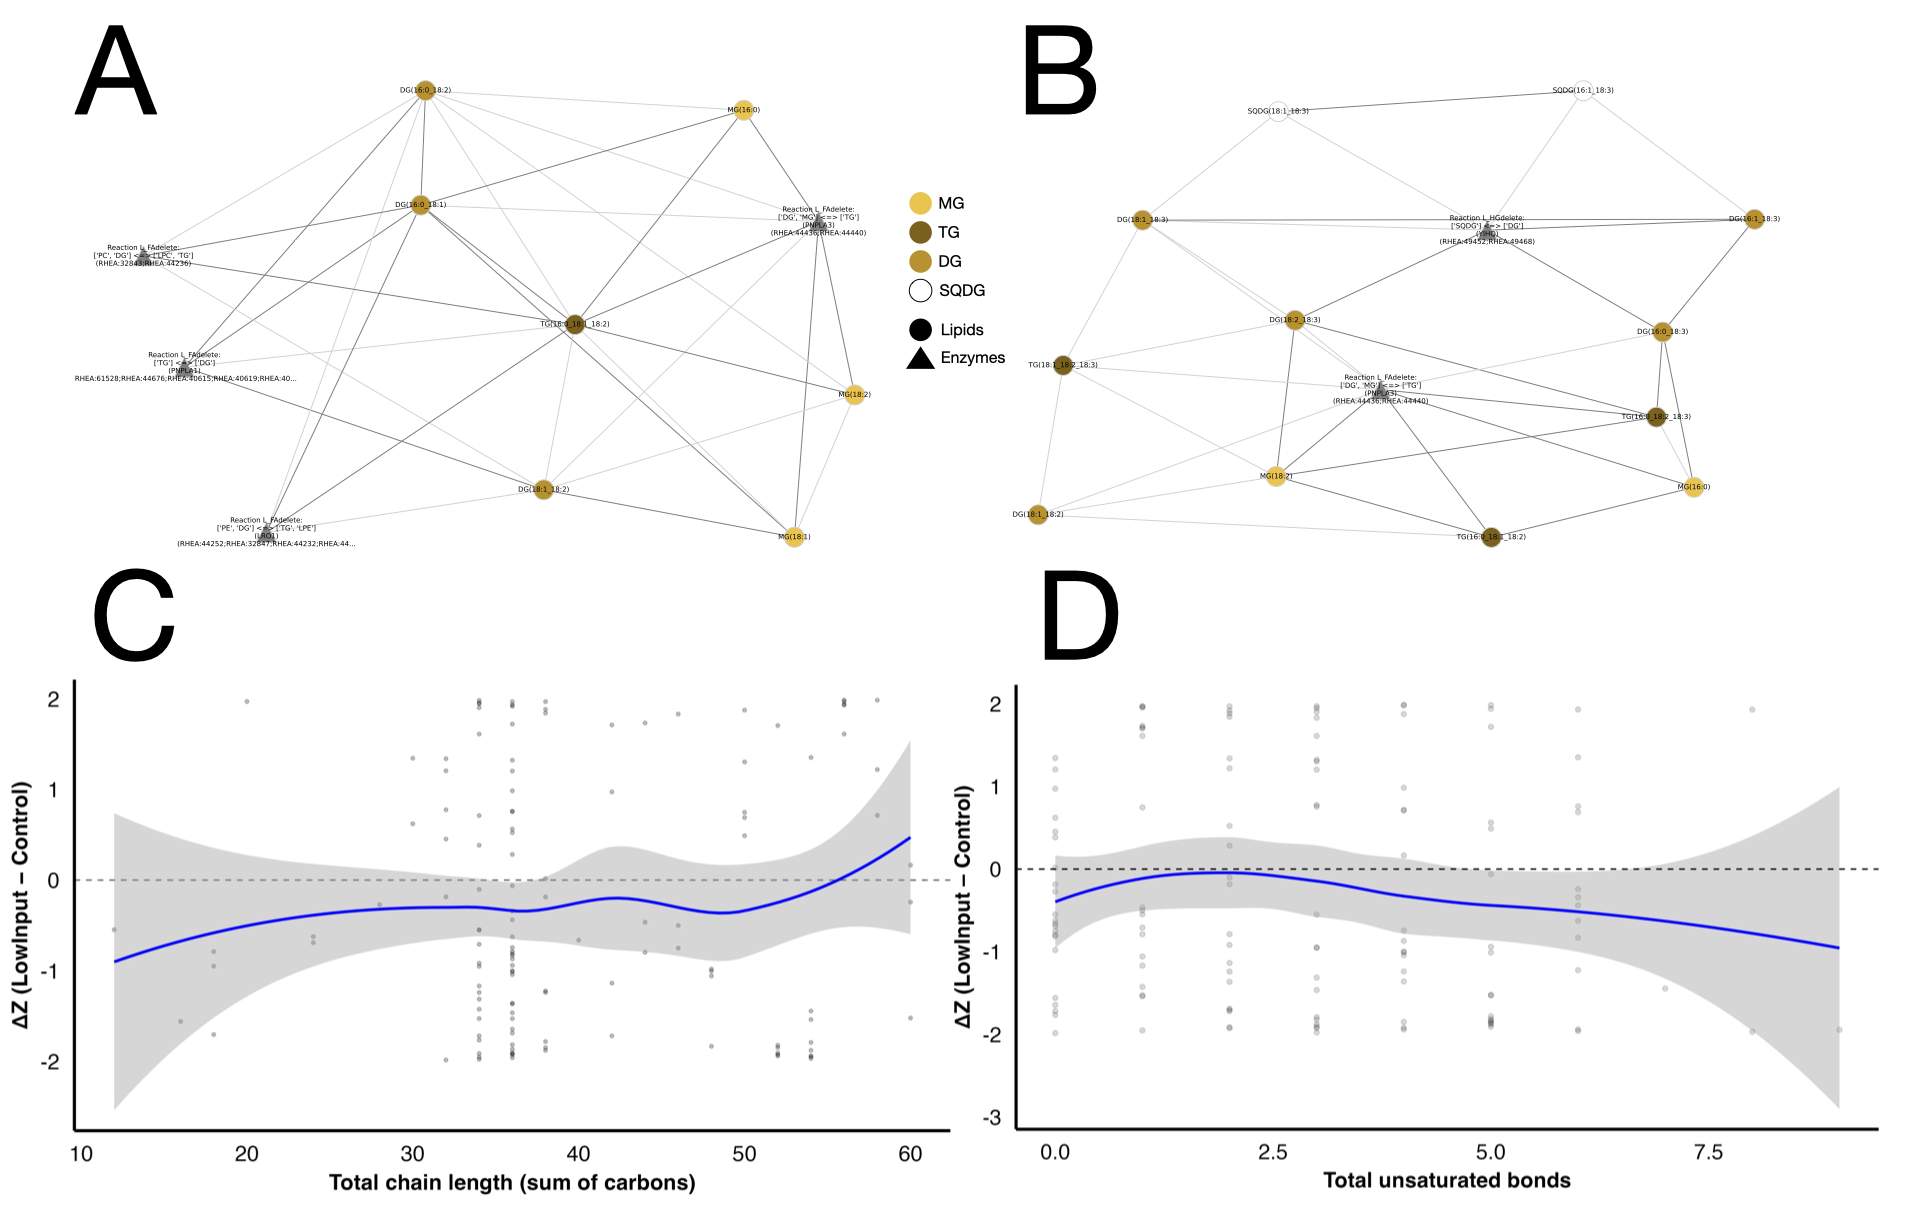
\includegraphics[width=\textwidth]{fig/main/Fig4.png} % <- your composite with A–D
  \caption{\textbf{Network enrichment and chain/unsaturation trends under low input.}
  \textbf{(A)} LINEX$^2$ lipid–enzyme network enrichment using \emph{ratio} contrasts between lipid classes; nodes are lipids (circles) colored by class (MG, DG, TG, SQDG) and enzymes (triangles), edges are curated conversions. Node size scales with absolute enrichment score.
  \textbf{(B)} LINEX$^2$ enrichment using \emph{absolute differences} (LowInput$-$Control) at the species level; same glyphs and legend as in (A).
  \textbf{(C)} Condition effect versus total chain length: points are individual lipid species and the blue line is a LOESS smoother ($\pm$~95\% CI in gray) of $\Delta Z = Z_{\mathrm{LowInput}} - Z_{\mathrm{Control}}$ plotted against the sum of acyl carbons. The curve dips below zero for mid chain lengths (C\,$\sim$\,34–50) and rises toward very long chains (C\,$\sim$\,56–60), consistent with loss of membrane lipids and relative enrichment of long-chain TAG. 
  \textbf{(D)} Condition effect versus total unsaturation (sum of double bonds). The downward trend indicates preferential depletion of highly unsaturated species under low input. 
  For (C–D), intensities were TIC-normalized, log-transformed with a small sample-wise pseudocount, $Z$-scored within condition and lipid, and then differenced (LowInput$-$Control) per species; the smoother was fit with LOESS (span~0.9). MG, DG, TG, SQDG: mono/di/triacylglycerol and sulfoquinovosyldiacylglycerol.}
  \label{fig:Fig4}
\end{figure*}

\subsection*{Integrated Lipid‐Metabolism Network, Ontology Enrichment, and GWAS Analaysis Idenfies Key Lipid Transitions Under Low Input}

As depicted in Figure \ref{fig:Fig}A and \ref{fig:Fig4}B, our combined enzyme-reaction network, lipid enrichment analysis, and genome-wide signals elucidate the interactions between DGs, MGs, TGs, PEs, and SQDGs. Nine pivotal pathways are identified, as demonstrated in Table \ref{tab:linex_reactions}.

\begin{table}[!ht]
  \centering
  \footnotesize
  \setlength{\tabcolsep}{4pt}
  \renewcommand{\arraystretch}{1.2}
  \caption{\textbf{Key enriched reactions in the LINEX2 sub-network (low-input vs.\ control)}}
  \label{tab:linex_reactions}
  \begin{tabularx}{\linewidth}{@{}%
      p{0.18\linewidth}
      p{0.22\linewidth}
      p{0.26\linewidth}
      X
    @{}}
    \toprule
    \textbf{Pathway} & \textbf{Stoichiometry} & \textbf{Putative enzyme(s)} & \textbf{Interpretation (low-input)} \\
    \midrule
    Lipolysis axis
      & DG $\rightarrow$ MG + FA
      & LIPE-like lipase
      & Provides MG for re-esterification or signalling. \\
    & MG + FA $\rightarrow$ TG
      & \textit{PNPLA3} (triacylglycerol synthase)
      & \textbf{$\downarrow$ flux}: storage synthesis suppressed. \\
    & TG $\rightarrow$ DG + FA
      & \textit{PNPLA1} (SORBI\_3001G041900)
      & \textbf{$\uparrow$ lipolysis}: dominant driver of DG pool. \\
    \addlinespace
    Phospholipid recycling
      & PE + DG $\rightleftharpoons$ LPE + TG
      & LRO1-type acyltransferase
      & Membrane PE shuttles acyl chains to TG. \\
    \addlinespace
    Plastid sulfolipid (SQDG) cycling
      & DG + UDP–sulfoquinovose $\rightarrow$ SQDG + UDP
      & \textit{SQD2} (sulfoquinovosyldiacylglycerol synthase)
      & Builds anionic sulfolipid in thylakoid membranes; phosphate-sparing replacement of phospholipids. \\
    & SQDG + H$_2$O $\rightarrow$ DG + sulfoquinovose
      & Putative sulfoquinovosidase (\textit{YihQ}-like)
      & SQDG turnover can release DG for TG/phospholipid remodeling; adjusts anionic lipid pool under stress. \\
    \addlinespace
    Alternative TG conversions
      & PE $\rightarrow$ DG + PI (acyl transfer)
      & EPTB (phosphoethanolamine phosphotransferase)
      & Recycles PE headgroups into TG $\Rightarrow$ DG cascade. \\
    & TG $\rightarrow$ RHEA:32843
      & Unspecified lipase
      & Alternative TG hydrolysis branch. \\
    & LPC $\leftrightarrow$ DG
      & Unspecified transferase
      & LPC\,$\leftrightarrow$\,DG interconversion at droplet surface. \\
    \bottomrule
  \end{tabularx}
\end{table}


The conversion of TG to DG catalyzed by PNPLA1 is identified as a critical process, complemented by the transformation from DG to TG facilitated by PNLPLA3. This enzymatic relationship suggests that modifications in TG turnover via PNPLA1 could account for the observed variations in lipid profiles (Fig X) when contrasting LI conditions to the C.

Additionally, the LION lipid-ontology enrichment analysis (Figure \ref{fig:}B) identifies significant terms such as "triacylglycerols [GL0301]" (FDR = 0.002), "lipid storage" (FDR = 0.008), "lipid droplet" (FDR = 0.008), "headgroup with neutral charge" (FDR = 0.012), and "glycerolipids [GL]" (FDR = 0.015) at a significance threshold of (−log₁₀ q > 1.3). These enriched terms suggest the accumulation and mobilization of TG pools, aligning with the biochemical roles of PNPLA1 and PNPLA3 in the recycling of triglycerides and diglycerides (TG~$\leftrightarrow$~DG):

\begin{array}{rcl}
\text{TG} & 
  \overset{\text{PNPLA3}}{\underset{\text{PNPLA1}}{\rightleftharpoons}} & 
\text{DG} \quad \xrightarrow{\text{}} \quad \text{TG/DG recycling}
\end{array}
\]

Furthermore, five independent GWAS results for TGs (Figure \ref{fig:Fig6}C) consistently identify a single locus on chromosome 1 annotated as the triacylglycerol lipase gene SORBI\_3001G041900 (SbPNPLA1) above the pvalue cutoffe Sum\_TG, TG\_54\_6, TG\_54\_7, TG\_56\_4, and TG\_56\_6 plots. The recurrent emergence of this peak across both aggregate and individual species traits highlights the crucial role of PNPLA1 in triacylglycerol homeostasis. Collectively, these findings support a model wherein genetic variation at the PNPLA1 locus directs the variability in lipid storage and mobilization, especially under cold and nutrient-deficient conditions.

\subsection*{}




\subsection*{Integrated LION, LINEX2, and GWAS Analyses Reveal Lipid Remodeling Under Lowinput}

Across three orthogonal readouts—reaction topology (LINEX2), lipid ontology (LION), and genetics (GWAS)—low-input consistently resolves to a lipolysis–re-acylation program that reallocates acyl chains from membranes into neutral storage while plastids tune their anionic surface by turning over SQDG. In the LINEX2 sub-network (Fig.\ \textbf{A–B}), the most connected transitions form a TG$\leftrightarrow$DG core coupled to acyl-editing links between phospholipids and neutral lipids (e.g., \mbox{PE + DG $\rightleftharpoons$ LPE + TG} and \mbox{LPC $\leftrightarrow$ DG}) and to a plastid branch that interconverts DG and SQDG via sulfoquinovose. LION enrichment reinforces this same architecture: terms related to glycerolipids, lipid droplets, and neutral headgroups are elevated in low-input, whereas multiple glycerophospholipid classes and membrane biophysical signatures (intrinsic curvature, lateral diffusion, transition temperature) trend downward (Fig.\ \textbf{B}). The class/subclass compositions match these directions: in Fig.\ \textbf{1A}, TG increases (2.7\%$\rightarrow$5.4\%) with a modest DG rise (13.8\%$\rightarrow$14.8\%); PE rises (5.8\%$\rightarrow$6.6\%), while plastid SQDG decreases (2.9\%$\rightarrow$1.4\%); MGDG decreases (34.5\%$\rightarrow$32.1\%); PC shows a mild decrease (25.6\%$\rightarrow$24.8\%); DGDG is essentially flat (12.7\%$\rightarrow$13.0\%). Subclass bars (Fig.\ \textbf{S5B–C}) echo this: glycerolipids show TG up (4.0\%$\rightarrow$7.9\%) and DG up (20.3\%$\rightarrow$21.9\%) with MGDG and SQDG down (50.6\%$\rightarrow$47.3\%; 4.3\%$\rightarrow$2.0\%), and the phospholipid pool tilts from PC toward PE (PC 79.9\%$\rightarrow$76.9\%; PE 18.4\%$\rightarrow$20.8\%), alongside small PG/LPC increases (LPE, PA $<0.1\%$). Together, these orthogonal signals point to acyl flux from structural phospholipids (especially PC) and plastid galactolipids/sulfolipids toward neutral TG, with PE and lysophospholipid edits mediating the transfer.

Genetic associations place enzyme “handles’’ directly onto the enriched edges and rationalize the species-level patterns. A patatin-like lipase, \textit{PNPLA1} (SORBI\_3001G041900), associates with twelve TG species (e.g., TG(18{:}1\_18{:}2\_18{:}3), TG(16{:}0\_18{:}1\_22{:}0)), fitting the TG$\rightarrow$DG$+$FA arm of the cycle and explaining the slight DG accumulation that feeds downstream edits or plastid demand. Re-esterification back to TG is anchored by \textit{DGAT1}/TAG1 (SORBI\_3010G170000) and \textit{DGAT3} (SORBI\_3009G034600), whose hits span MG, DGDG(16{:}0\_18{:}3), and multiple TGs; the \textit{DGAT3} bias toward polyunsaturated TGs is consistent with the smooth trends versus chain length/unsaturation (Fig.\ \textbf{C–D}) characteristic of storage-oriented remodeling. On the plastid branch, \textit{SQD2} (SORBI\_3001G427300) maps to SQDG(16{:}0\_16{:}0 / 16{:}0\_18{:}1 / 16{:}0\_18{:}3) (and one TG), exactly the DG$\rightarrow$SQDG step; the observed SQDG decrease with low-input suggests heightened turnover/substitution that spares phosphate and adjusts the thylakoid surface charge while competing with DGAT for DG. A \textit{PLD} locus (SORBI\_3005G222500) linked to DG and TG species provides a membrane-to-DG route via PA$\rightarrow$DG (PAP), supplying substrate both for DGAT (storage) and \textit{SQD2} (plastid). Finally, two broad LCAT-like associations—\textit{LCAT-like 4} (SORBI\_3006G214500; 22 hits across MG, DG, TG, PC/PE/PG, MGDG/DGDG, SQDG) and \textit{LCAT-like 1} (SORBI\_3001G103800; PC and TG hits)—fit the lysophospholipid acyl-shuttling implicit in the \mbox{LPC $\leftrightarrow$ DG} and \mbox{PG + DG $\rightleftharpoons$ LPC + TG} edges and help explain the modest PC$\downarrow$/PE$\uparrow$ tilt.

In sum, low-input triggers a coherent remodeling program in which PNPLA1-mediated TG breakdown, DGAT1/3-mediated TG synthesis, PLD/PAP-derived DG supply, LCAT-like acyl editing, and plastid \textit{SQD2} draw on the same DG node. The net effect is redistribution of acyl chains from phospholipids and plastid galacto/sulfolipids into neutral TG, with plastids concurrently substituting SQDG for phosphate-demanding anionic phospholipids. The integrated evidence—enriched reaction paths (Fig.\ \textbf{A–B}), ontology shifts (Fig.\ \textbf{B}), class/subclass compositions (Fig.\ \textbf{1A}, \textbf{S5B–C}), and species-level smooths (Fig.\ \textbf{C–D})—all point to this same lipolysis–re-acylation switch and SQDG cycling as hallmarks of the low-input state.


\begin{figure}[!ht]
  \centering
  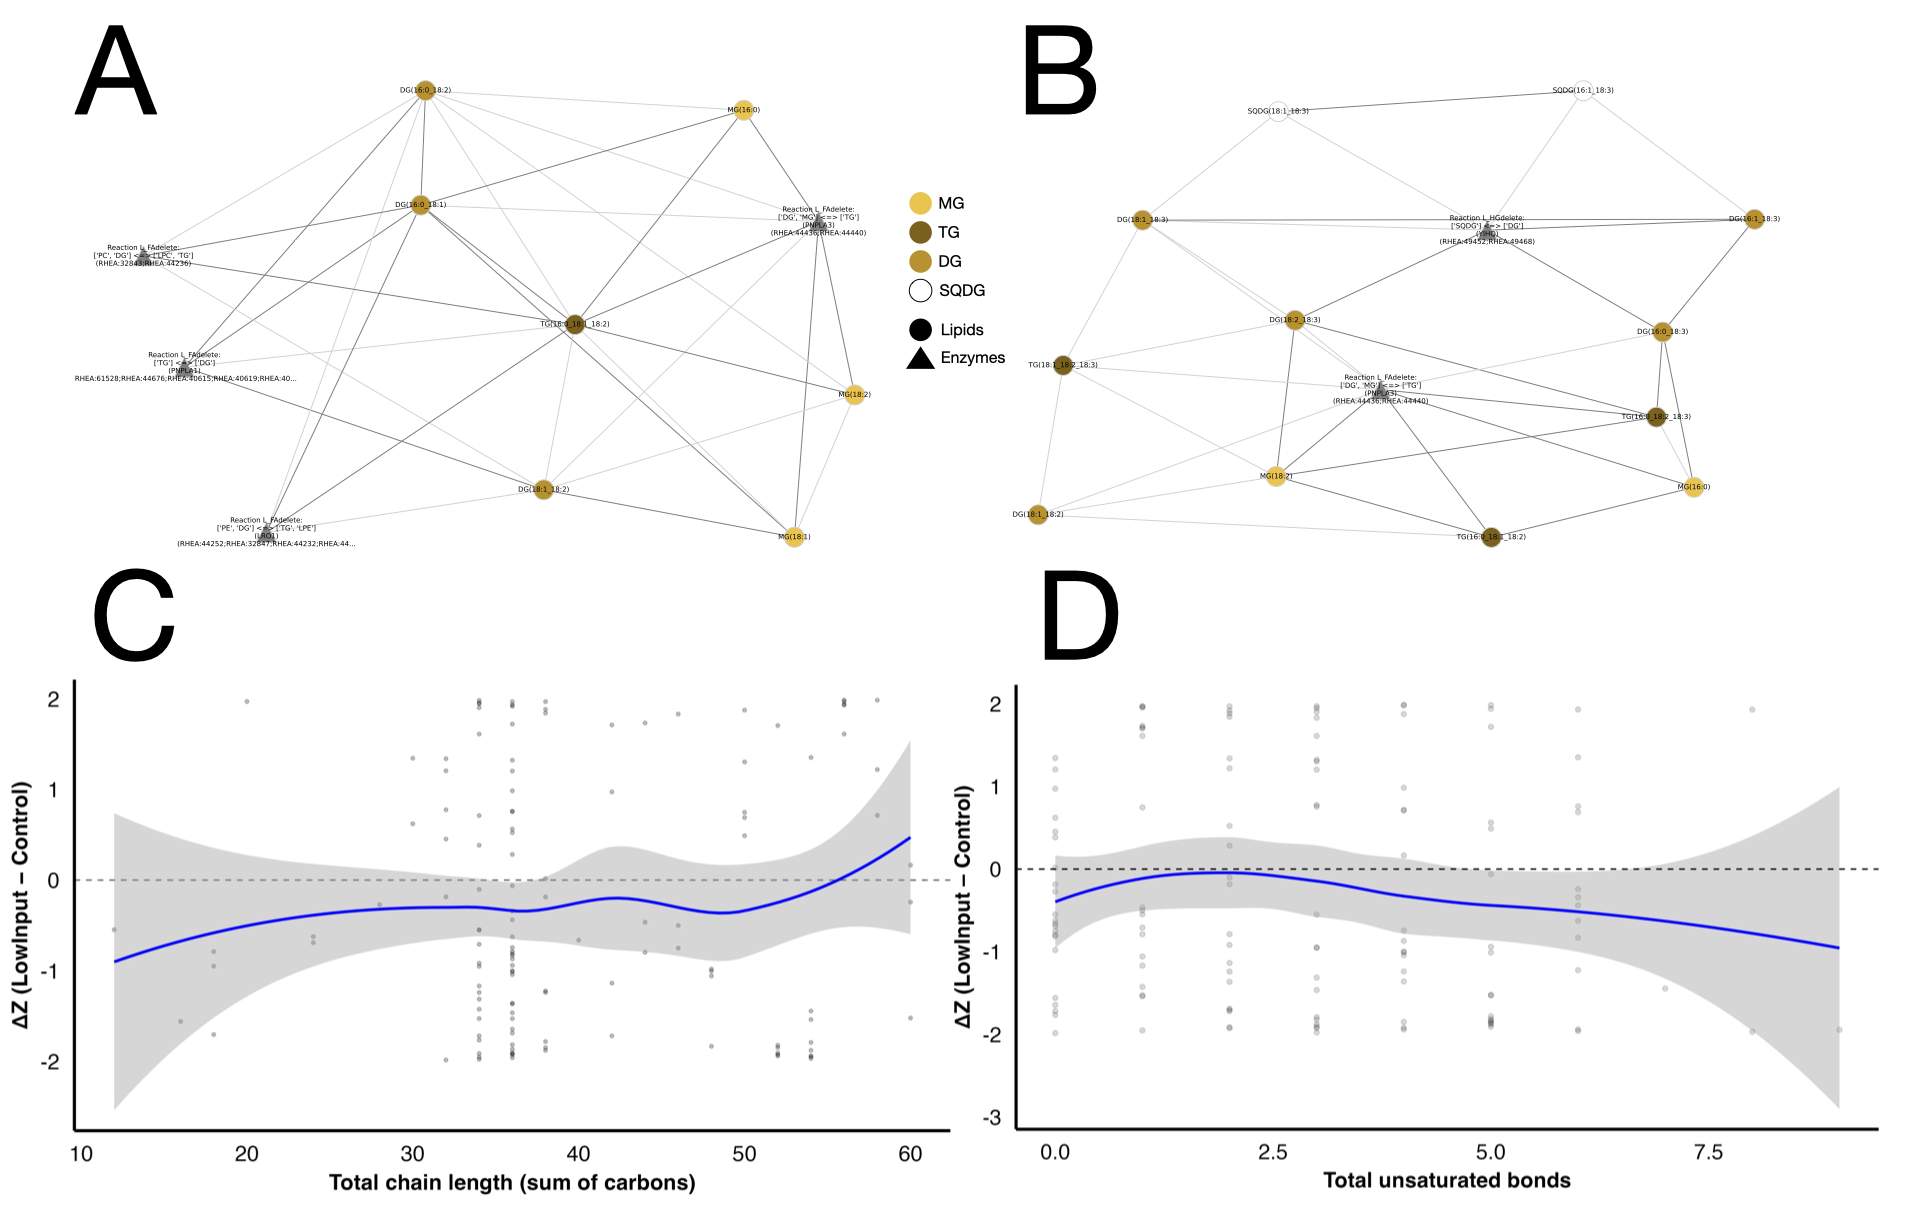
\includegraphics[width=\linewidth]{fig/main/Fig4.png}
  \caption{\textbf{Random-forest pipeline: residualization, model performance, and SHAP-based interpretation.}
  \textbf{A}, Kernel-density plots of the phenotype (example: plant height) before (purple) and after PC residualization (yellow). Residualization collapses population-structure variation and recenters values near zero while retaining spread/ordering needed for prediction. 
  \textbf{B}, Example lipid (TG(10:0/10:0/10:0)) before (purple) and after PC residualization (yellow). Changes are modest relative to the phenotype, indicating that lipid variance is largely biological once PC effects are removed. 
  \textbf{C}, Five-fold cross-validation on the training set for the tuned random forest (1{,}000 trees); points show per-fold RMSE, MAE, and $R^2$, with dashed lines marking fold means, demonstrating stable generalization across folds. 
  \textbf{D}, Held-out test performance: RF predictions versus observed residual phenotype, with the 1:1 line shown (dashed). The model attains RMSE $\approx 24.2$ and $R^2 \approx 0.69$. 
  \textbf{E}, TreeSHAP interpretation of the final model. Left, beeswarm: each point is a sample’s SHAP value for the top features (color encodes standardized abundance); positive values increase the predicted residual phenotype. Right, global ranking by mean absolute SHAP identifies the most phenotype-informative lipids (notably several short/medium-chain TG species alongside selected membrane lipids such as PC/PE, MGDG, and SQDG). 
  Together, the panels show that PC residualization removes confounding, the RF model generalizes, and SHAP pinpoints the lipid species that most strongly drive predictions.}
  \label{fig:fig4_rf_shap}
\end{figure}



\subsection*{Integrated Lipid‐Metabolism Network, Ontology Enrichment, and GWAS Analaysis Idenfies Key Lipid Transitions Under Low Input}


\noindent \textbf{Network-level shifts (LINEX2).}
The reaction sub-network enriched in low-input samples is dominated by a lipolysis–re-acylation axis that shuttles acyl chains between membranes and storage (Fig.\ \textbf{A–B}). Three features stand out:
\begin{enumerate}\itemsep3pt
  \item \textbf{TG $\leftrightarrow$ DG cycling.} Reactions converting triacylglycerol (TG) to diacylglycerol (DG) {+} free fatty acid (FA), and the reverse re-esterification of MG/DG back to TG, are over-represented, indicating active remodeling of the neutral-lipid pool.
  \item \textbf{Phospholipid $\leftrightarrow$ neutral-lipid crosstalk.} The edge \mbox{PE + DG $\rightleftharpoons$ LPE + TG} suggests a PE-based acyl-transfer route that moves acyl chains from membrane glycerophospholipids into TG (a Lands–cycle–like edit). The \mbox{LPC $\leftrightarrow$ DG} connection is consistent with lysophospholipid acyl transfer at the droplet surface.
  \item \textbf{Plastid anionic-lipid cycling.} \mbox{DG + UDP–sulfoquinovose $\rightarrow$ SQDG + UDP}, and the reverse hydrolytic route \mbox{SQDG + H$_2$O $\rightarrow$ DG + sulfoquinovose}, indicate dynamic sulfoquinovosyldiacylglycerol (SQDG) turnover—i.e., plastid membranes swapping phosphate-containing anionic lipids for SQDG and feeding DG back to the glycerolipid pool when needed.
\end{enumerate}

\noindent \textbf{Ontology-level consequences (LION).}
LION enrichment mirrors the network picture (Fig.\ \textbf{B}). Terms increased in low-input include \emph{glycerolipids} (DG/TG), \emph{lipid droplet}/\emph{lipid storage}, and \emph{headgroup with neutral charge}, consistent with accumulation of neutral storage lipids. Terms decreased include \emph{glycerophospholipids} (PC/PE subclasses) and membrane biophysical signatures (e.g., intrinsic curvature, lateral diffusion/transition-temperature terms), pointing to depletion or acyl editing of structural phospholipids. Together, these ontologies argue for redistribution of acyl chains from zwitterionic/anionic membrane lipids into storage TG, alongside plastid-specific adjustments.

\noindent \textbf{Genetic anchors (GWAS) that map onto the same reactions.}
GWAS hits pin enzymes to the enriched edges and explain species-level patterns:
\begin{itemize}\itemsep3pt
  \item \textbf{TG lipolysis $\rightarrow$ DG + FA: \textit{PNPLA1} (SORBI\_3001G041900).} Associations to 12 TG species (e.g., TG(18:1\_18:2\_18:3), TG(16:0\_18:1\_22:0)) implicate a patatin-like lipase in the TG$\rightarrow$DG arm highlighted by LINEX2, shifting the DG/TG balance and feeding DG into downstream editing or SQDG synthesis.
  \item \textbf{DG + acyl–CoA $\rightarrow$ TG: \textit{DGAT1}/TAG1 (SORBI\_3010G170000) and \textit{DGAT3} (SORBI\_3009G034600).} Hits spanning MG, DGDG(16:0\_18:3) and multiple TGs (with \textit{DGAT3} biased to polyunsaturated TGs) anchor re-esterification back to TG and help explain the chain/unsaturation smooths (Fig.\ \textbf{C–D}).
  \item \textbf{DG + UDP–sulfoquinovose $\rightarrow$ SQDG + UDP: \textit{SQD2} (SORBI\_3001G427300).} Associations with SQDG(16:0\_16:0/16:0\_18:1/16:0\_18:3) (and one TG) fit the plastid branch; \textit{SQD2} builds sulfolipid in thylakoids, likely sparing phosphate and tuning anionic surface charge under low-input while competing with DGAT for the DG substrate.
  \item \textbf{PC/PE $\rightarrow$ PA + headgroup: \textit{PLD} (SORBI\_3005G222500).} Links to DG and TG species suggest PLD-derived PA, dephosphorylated to DG (via PAP), supplies DG for DGAT or for \textit{SQD2}—exactly the membrane-to-storage trafficking seen in LINEX2 and LION.
  \item \textbf{Lysophospholipid acyl transfer / acyl editing: LCAT-like enzymes.} 
  \textit{LCAT-like 4} (SORBI\_3006G214500; 22 hits across MG, DG, TG, PC/PE/PG, MGDG/DGDG, SQDG) and \textit{LCAT-like 1} (SORBI\_3001G103800; PC and TG hits) are consistent with phospholipid$\rightarrow$neutral-lipid acyl flow and the \mbox{LPC $\leftrightarrow$ DG} / \mbox{PG + DG $\rightleftharpoons$ LPC + TG} edges.
\end{itemize}

\noindent \textbf{Composition evidence (stacked bars) supports the model.}
Class-level composition (Fig.\ \textbf{1A}) shows \textbf{TG increase} (2.7\% $\rightarrow$ 5.4\%), \textbf{DG slight increase} (13.8\% $\rightarrow$ 14.8\%), \textbf{PE increase} (5.8\% $\rightarrow$ 6.6\%), and \textbf{SQDG decrease} (2.9\% $\rightarrow$ 1.4\%), with \mbox{MGDG decrease} (34.5\% $\rightarrow$ 32.1\%), mild \mbox{PC decrease} (25.6\% $\rightarrow$ 24.8\%), and DGDG $\sim$stable (12.7\% $\rightarrow$ 13.0\%). 
Subclass panels corroborate this: glycerolipids (S5B) show \textbf{TG up} (4.0\% $\rightarrow$ 7.9\%) and \textbf{DG up} (20.3\% $\rightarrow$ 21.9\%), with \textbf{MGDG down} (50.6\% $\rightarrow$ 47.3\%) and \textbf{SQDG down} (4.3\% $\rightarrow$ 2.0\%); phospholipids (S5C) show a \textbf{PC$\downarrow$ / PE$\uparrow$ tilt} (PC 79.9\% $\rightarrow$ 76.9\%; PE 18.4\% $\rightarrow$ 20.8\%), small PG and LPC increases, LPE/PA $<0.1\%$.

\noindent \textbf{Synthesis and interpretation.}
Across three orthogonal layers, low-input drives a coherent remodeling program: (\emph{i}) enhanced TG$\leftrightarrow$DG cycling; (\emph{ii}) PE-mediated acyl transfer into TG and LPC/DG interconversion; and (\emph{iii}) plastid SQDG cycling that competes with DGAT for DG. The composition and ontology shifts (neutral lipids and droplets up; phospholipid/biophysical signatures down; SQDG/galactolipids reduced) and the genetic anchors (\textit{PNPLA1}, \textit{DGAT1/3}, \textit{SQD2}, \textit{PLD}, LCAT-like enzymes) converge on the same mechanism. We propose that, under low-input, plants reallocate acyl chains from structural phospholipids to storage TG while plastids substitute SQDG for phosphate-demanding anionic phospholipids. The species-level smooths versus chain length and unsaturation (Fig.\ \textbf{C–D}) are consistent with storage-oriented remodeling into variably unsaturated, sometimes longer-chain TGs, with relative depletion/editing of membrane PCs/PEs and plastid galactolipids.








%--------------------------------------------------------------------
\bibliographystyle{plainnat}
\bibliography{lipid_refs}



\section*{Discussion}
Something something lipids are good. 


\section*{Conclusion}

because we can For more information, see \nameref{S1_Appendix}.

\section*{Supporting information}

% Include only the SI item label in the paragraph heading. Use the \nameref{label} command to cite SI items in the text.
\paragraph*{S1 Fig.}
\label{S1_Fig}
{\bf Bold the title sentence.} Add descriptive text after the title of the item (optional).

\paragraph*{S2 Fig.}
\label{S2_Fig}
{\bf Lorem ipsum.} Maecenas convallis mauris sit amet sem ultrices gravida. Etiam eget sapien nibh. Sed ac ipsum eget enim egestas ullamcorper nec euismod ligula. Curabitur fringilla pulvinar lectus consectetur pellentesque.

\paragraph*{S1 File.}
\label{S1_File}
{\bf Lorem ipsum.}  Maecenas convallis mauris sit amet sem ultrices gravida. Etiam eget sapien nibh. Sed ac ipsum eget enim egestas ullamcorper nec euismod ligula. Curabitur fringilla pulvinar lectus consectetur pellentesque.

\paragraph*{S1 Video.}
\label{S1_Video}
{\bf Lorem ipsum.}  Maecenas convallis mauris sit amet sem ultrices gravida. Etiam eget sapien nibh. Sed ac ipsum eget enim egestas ullamcorper nec euismod ligula. Curabitur fringilla pulvinar lectus consectetur pellentesque.

\paragraph*{S1 Appendix.}
\label{S1_Appendix}
{\bf Lorem ipsum.} Maecenas convallis mauris sit amet sem ultrices gravida. Etiam eget sapien nibh. Sed ac ipsum eget enim egestas ullamcorper nec euismod ligula. Curabitur fringilla pulvinar lectus consectetur pellentesque.

\paragraph*{S1 Table.}
\label{S1_Table}
{\bf Lorem ipsum.} Maecenas convallis mauris sit amet sem ultrices gravida. Etiam eget sapien nibh. Sed ac ipsum eget enim egestas ullamcorper nec euismod ligula. Curabitur fringilla pulvinar lectus consectetur pellentesque.

\section*{Acknowledgments}
Me, myself and I

\nolinenumbers

% Either type in your references using
% \begin{thebibliography}{}
% \bibitem{}
% Text
% \end{thebibliography}
%
% or
%
% Compile your BiBTeX database using our plos2015.bst
% style file and paste the contents of your .bbl file
% here. See http://journals.plos.org/plosone/s/latex for 
% step-by-step instructions.
% 
\begin{thebibliography}{10}


\bibitem[Dall’Osto \emph{et~al.}(2012)]{DallOsto2012}
Dall’Osto, L., Cazzaniga, S., Bressan, M., Paleček, D., Židek, K., Jennings, R.~C., \& Bassi, R. (2012).  
Zeaxanthin protects plant photosynthesis by modulating chlorophyll triplet yield in specific light‐harvesting antenna subunits.  
\emph{Journal of Biological Chemistry}, 287(10), 6180–6190.

\bibitem[Demmig‐Adams \emph{et~al.}(2020)]{DemmigAdams2020}
Demmig‐Adams, B., Adams, W.~W., III, \& Holzwarth, A.~R. (2020).  
Zeaxanthin, a molecule for photoprotection in many different environments.  
\emph{Molecules}, 25(1), 100.

\bibitem[Guardini \emph{et~al.}(2020)]{Guardini2020}
Guardini, Z., Bressan, M., Caferri, R., Bassi, R., \& Dall’Osto, L. (2020).  
Identification of a pigment cluster catalysing fast photoprotective quenching response in CP29.  
\emph{Nature Plants}, 6, 1261–1273.


\bibitem[Williams and Morgan(1979)]{Williams1979}
Williams, E.~A., \& Morgan, P.~W. (1979).  
Floral initiation in sorghum hastened by gibberellic acid and far‐red light.  
\emph{Planta}, 145, 269–272.

\bibitem[Lee \emph{et~al.}(1998)]{Lee1998}
Lee, I.~J., Foster, K.~R., \& Morgan, P.~W. (1998).  
Photoperiod control of gibberellin levels and flowering in sorghum.  
\emph{Plant Physiology}, 116, 1003–1011.

\bibitem[Paul \emph{et~al.}(2020)]{Paul2020}
Paul, P., Dhatt, B.~K., Miller, M., \emph{et~al.} (2020).  
MADS78 and MADS79 are essential regulators of early seed development in rice.  
\emph{Plant Physiology}, 182, 933–948.

\bibitem[Jabir and Mahmoud(2021)]{Jabir2021}
Jabir, D.~A.~A., \& Mahmoud, M.~R. (2021).  
The effect of temperature stress associated with different planting dates and levels of gibberellic acid on the growth of sorghum spring.  
\emph{IOP Conference Series: Earth and Environmental Science}, 923, 012090.

\bibitem[Young and Britton(1989)]{Young1989}
Young, A.~J., \& Britton, G. (1989).
\newblock The distribution of alpha-carotene in the photosynthetic pigment-protein complexes of higher plants.
\newblock \emph{Plant Science}, 64, 179–183.

\bibitem[Vishwakarma \emph{et~al.}(2015)]{Vishwakarma2015}
Vishwakarma, A., Tetali, S.~D., Selinski, J., Scheibe, R., \& Padmasree, K. (2015).
\newblock Importance of the alternative oxidase (AOX) pathway in regulating cellular redox and ROS homeostasis to optimize photosynthesis during restriction of the cytochrome oxidase pathway in \emph{Arabidopsis thaliana}.
\newblock \emph{Annals of Botany}, 116(4), 553–566.
\newblock \doi{10.1093/aob/mcv066}

\bibitem[Gandin \emph{et~al.}(2014)]{Gandin2014}
Gandin, A., Dinakar, C., McDonald, A.~E., \& Vanlerberghe, G.~C. (2014).
\newblock Cooperation between the AOX pathway and nitrate assimilation to maintain optimal photosynthesis by regulating the accumulation of reducing equivalents.
\newblock \emph{Plant Physiology}.
  
\bibitem[Sayeed \emph{et~al.}(2016)]{Sayeed2016}
Sayeed, M.~S.~B., \emph{et~al.} (2016).  
Critical analysis on characterization, systemic effect, and therapeutic potential of beta‑sitosterol.  
\emph{Medicines}.

\bibitem[Mueller and Brown(1980)]{Mueller1980}
Mueller, S.~C., \& Brown, R.~M., Jr. (1980).  
Evidence for an intramembrane component associated with a cellulose microfibril synthesizing complex in higher plants.  
\emph{Journal of Cell Biology}, 84(3), 315–326.

\bibitem[Somerville(2006)]{Somerville2006}
Somerville, C. (2006).  
Cellulose synthesis in higher plants.  
\emph{Annual Review of Cell and Developmental Biology}, 22, 53–78.

\bibitem[Hu \emph{et~al.}(2018)]{Hu2018}
Hu, H., \emph{et~al.} (2018).  
Cellulose synthase mutants distinctively affect cell growth and cell wall integrity for plant biomass production in Arabidopsis.  
\emph{Plant Cell Physiology}, 59(6), 1142–1154.

\bibitem[Arioli \emph{et~al.}(1998)]{Arioli1998}
Arioli, T., \emph{et~al.} (1998).  
Molecular analysis of cellulose biosynthesis in Arabidopsis.  
\emph{Science}, 279, 717–720.

\bibitem[Persson \emph{et~al.}(2007)]{Persson2007}
Persson, S., \emph{et~al.} (2007).  
Genetic evidence for three unique components in primary cell‐wall cellulose synthase complexes.  
\emph{Proceedings of the National Academy of Sciences USA}, 104(39), 15566–15571.

\bibitem[Cano‐Delgado \emph{et~al.}(2003)]{CanoDelgado2003}
Cano‐Delgado, A.~I., \emph{et~al.} (2003).  
Reduced cellulose synthesis invokes lignification and defense responses in Arabidopsis thaliana.  
\emph{Plant Journal}, 34(4), 351–362.

\bibitem[Hernández‐Blanco \emph{et~al.}(2007)]{HernandezBlanco2007}
Hernández‐Blanco, C., \emph{et~al.} (2007).  
Impaired cellulose synthesis enhances disease resistance in Arabidopsis.  
\emph{Plant Cell}, 19(3), 890–903.

\bibitem[Tomlinson \emph{et~al.}(2004)]{Tomlinson2004}
Tomlinson, K., \emph{et~al.} (2004).  
Effects of inhibiting cellulose biosynthesis on nitrogen, phosphorus, and sulfur metabolism in Brassica napus.  
\emph{Plant Physiology}, 134(2), 568–577.

\bibitem[Ekman \emph{et~al.}(2008)]{Ekman2008}
Ekman, D., \emph{et~al.} (2008).  
Carbon partitioning during secondary wall biosynthesis in Arabidopsis stems.  
\emph{Plant Journal}, 53(3), 425–436.

\bibitem[Iyer \emph{et~al.}(2008)]{Iyer2008}
Iyer, P.~V.~V., \emph{et~al.} (2008).  
Alteration of cellulose and lignin in Arabidopsis via RNAi of cellulose synthase genes.  
\emph{Molecular Plant}, 1(2), 212–220.

\bibitem[Shi \emph{et~al.}(2012)]{Shi2012}
Shi, D., \emph{et~al.} (2012).  
Genetic analysis of Arabidopsis cellulose mutants reveals secondary cell wall defects.  
\emph{Plant Physiology}, 158(4), 1587–1595.

\bibitem[Tan \emph{et~al.}(2011)]{Tan2011}
Tan, J., \emph{et~al.} (2011).  
Enhancing seed protein content by down‐regulating cellulose synthesis in rice.  
\emph{Plant Biotechnology Journal}, 9(7), 834–842.

\bibitem[Yoshie‐Stark \emph{et~al.}(2008)]{YoshieStark2008}
Yoshie‐Stark, Y., \emph{et~al.} (2008).  
Manipulation of cell wall composition to increase seed protein content in maize.  
\emph{Journal of Agricultural Food Chemistry}, 56(11), 3981–3988.

\bibitem[Knowles(1983)]{Knowles1983}
Knowles, N.~R. (1983).  
Carbohydrate and protein accumulation during seed development in peas.  
\emph{Plant Physiology}, 72(1), 45–50.

\bibitem[Hu \emph{et~al.}(2020)]{Hu2020}
Hu, H., \emph{et~al.} (2020).  
Manipulating cellulose synthase for seed storage protein improvement.  
\emph{Plant Cell Reports}, 39(5), 607–619.


\bibitem{Yu2002}
Yu, B., Xu, C., \& Benning, C. (2002).  
\emph{Arabidopsis disrupted in SQD2 encoding sulfolipid synthase is impaired in phosphate-limited growth.}  
\textit{Proceedings of the National Academy of Sciences USA}, 99, 5732–5737.

\bibitem{Sun2021}
Sun, Y., Song, K., Liu, L., \emph{et al.} (2021).  
\emph{Sulfoquinovosyl diacylglycerol synthase 1 impairs glycolipid accumulation and photosynthesis in phosphate-deprived rice.}  
\textit{Journal of Experimental Botany}, 72(18), 6510–6523.

\bibitem{Qin2015}
Qin, X., Suga, M., Kuang, T., \& Shen, J. R. (2015).  
\emph{Structural basis for energy transfer pathways in the plant PSI-LHCI supercomplex.}  
\textit{Science}, 348, 989–995.

\bibitem{Umena2011}
Umena, Y., Kawakami, K., Shen, J. R., \& Kamiya, N. (2011).  
\emph{Crystal structure of oxygen-evolving photosystem II at 1.9 Å resolution.}  
\textit{Nature}, 473, 55–60.

\bibitem{YuBenning2003}
Yu, B., \& Benning, C. (2003).  
\emph{Anionic lipids are required for chloroplast structure and function in Arabidopsis.}  
\textit{The Plant Journal}, 36, 762–770.

\bibitem{Essigmann1998}
Essigmann, B., Güler, S., Narang, R. A., Linke, D., \& Benning, C. (1998).  
\emph{Phosphate availability affects thylakoid lipid composition and the expression of SQD1, a gene required for sulfolipid biosynthesis in Arabidopsis thaliana.}  
\textit{Proceedings of the National Academy of Sciences USA}, 95, 1950–1955.

\bibitem{Nakamura2013}
Nakamura, Y. (2013).  
\emph{Phosphate starvation and membrane lipid remodeling in seed plants.}  
\textit{Progress in Lipid Research}, 52, 43–50.

\bibitem{Yang2011}
Yang, Y., Yu, X., Song, L., \& An, C. (2011).  
\emph{ABI4 Activates DGAT1 Expression in Arabidopsis Seedlings during Nitrogen Deficiency.}  
\textit{Plant Physiology}, 156(2), 874–883.

\bibitem{Tan2018}
Tan, W.-J., Yang, Y.-C., Zhou, Y., Huang, L.-P., Xu, L., Chen, Q.-F., Yu, L.-J., \& Xiao, S. (2018).  
\emph{DIACYLGLYCEROL ACYLTRANSFERASE and DIACYLGLYCEROL KINASE Modulate Triacylglycerol and Phosphatidic Acid Production in the Plant Response to Freezing Stress.}  
\textit{Plant Physiology}, 177(4), 1304–1316.

\bibitem{Zhang2009}
Zhang, M., Fan, J., Taylor, D. C., \& Ohlrogge, J. B. (2009).  
\emph{DGAT1 and PDAT1 Acyltransferases Have Overlapping Functions in Arabidopsis Triacylglycerol Biosynthesis and Are Essential for Normal Pollen and Seed Development.}  
\textit{The Plant Cell}, 21(12), 3885–3901.

\end{thebibliography}

%==========================================
%   Start the Supplementary Material section
%==========================================
\FloatBarrier
\section*{Supplementary Material}
\beginsupplement


%========================================================
%  Supplementary Figure S1 – TIC traces
%========================================================
\begin{figure}[htp]
  \centering
  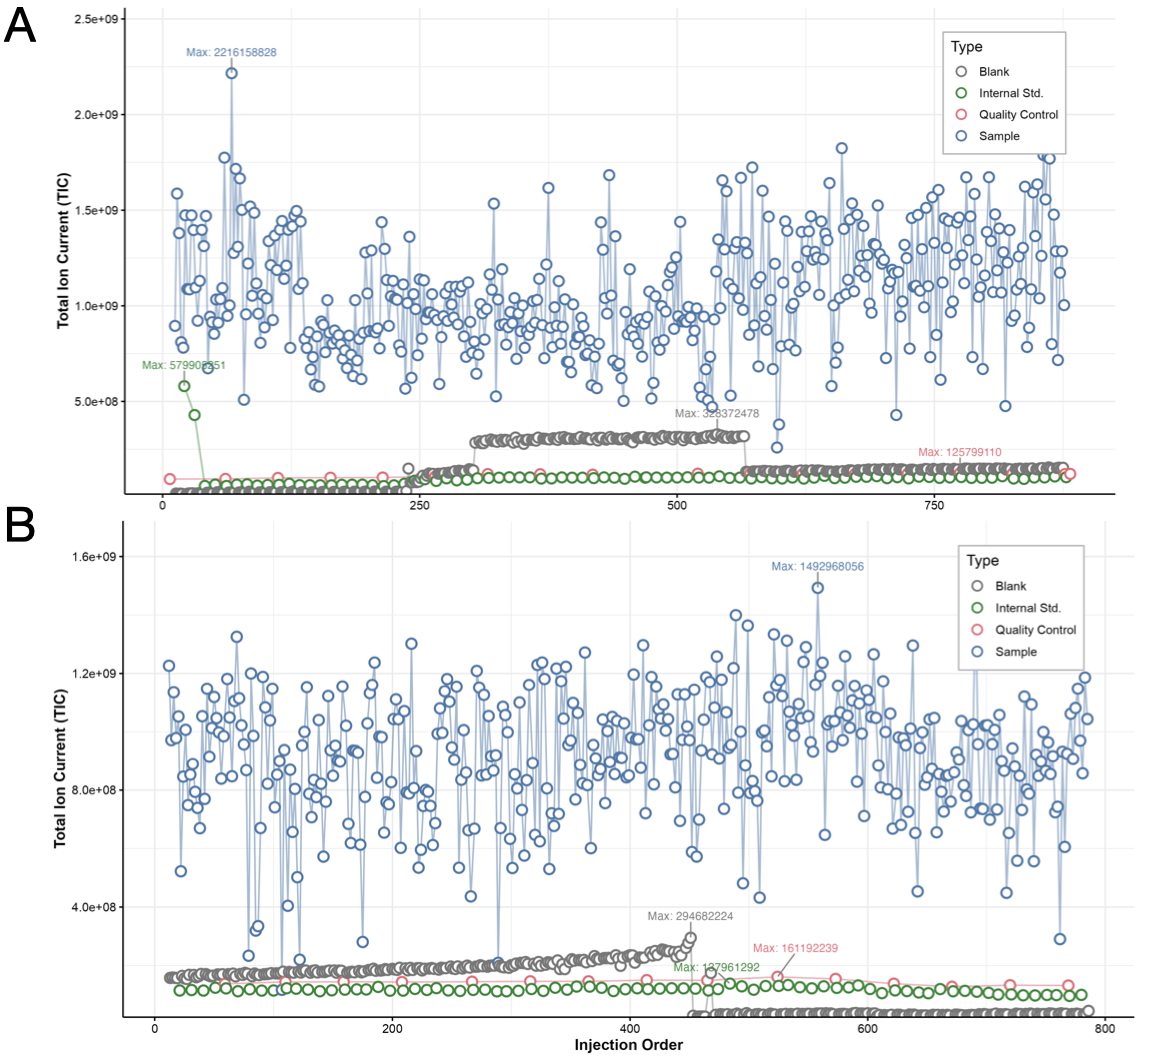
\includegraphics[width=\textwidth]{fig/supp/SuppFig1.png}
  \caption{
    Total ion current (TIC) traces for all injections in the lipidomics run. 
    {\bf(A)} Control samples (top panel). 
    {\bf(B)} Lowinput samples (bottom panel).
  }
  \label{fig:S1}
\end{figure}



%========================================================
%  Supplementary Figure S2 - SERFF RSD & PCA results
%========================================================
\begin{figure}[htp]
  \centering
  % Combined panel A (left) and B (right) in one image file
  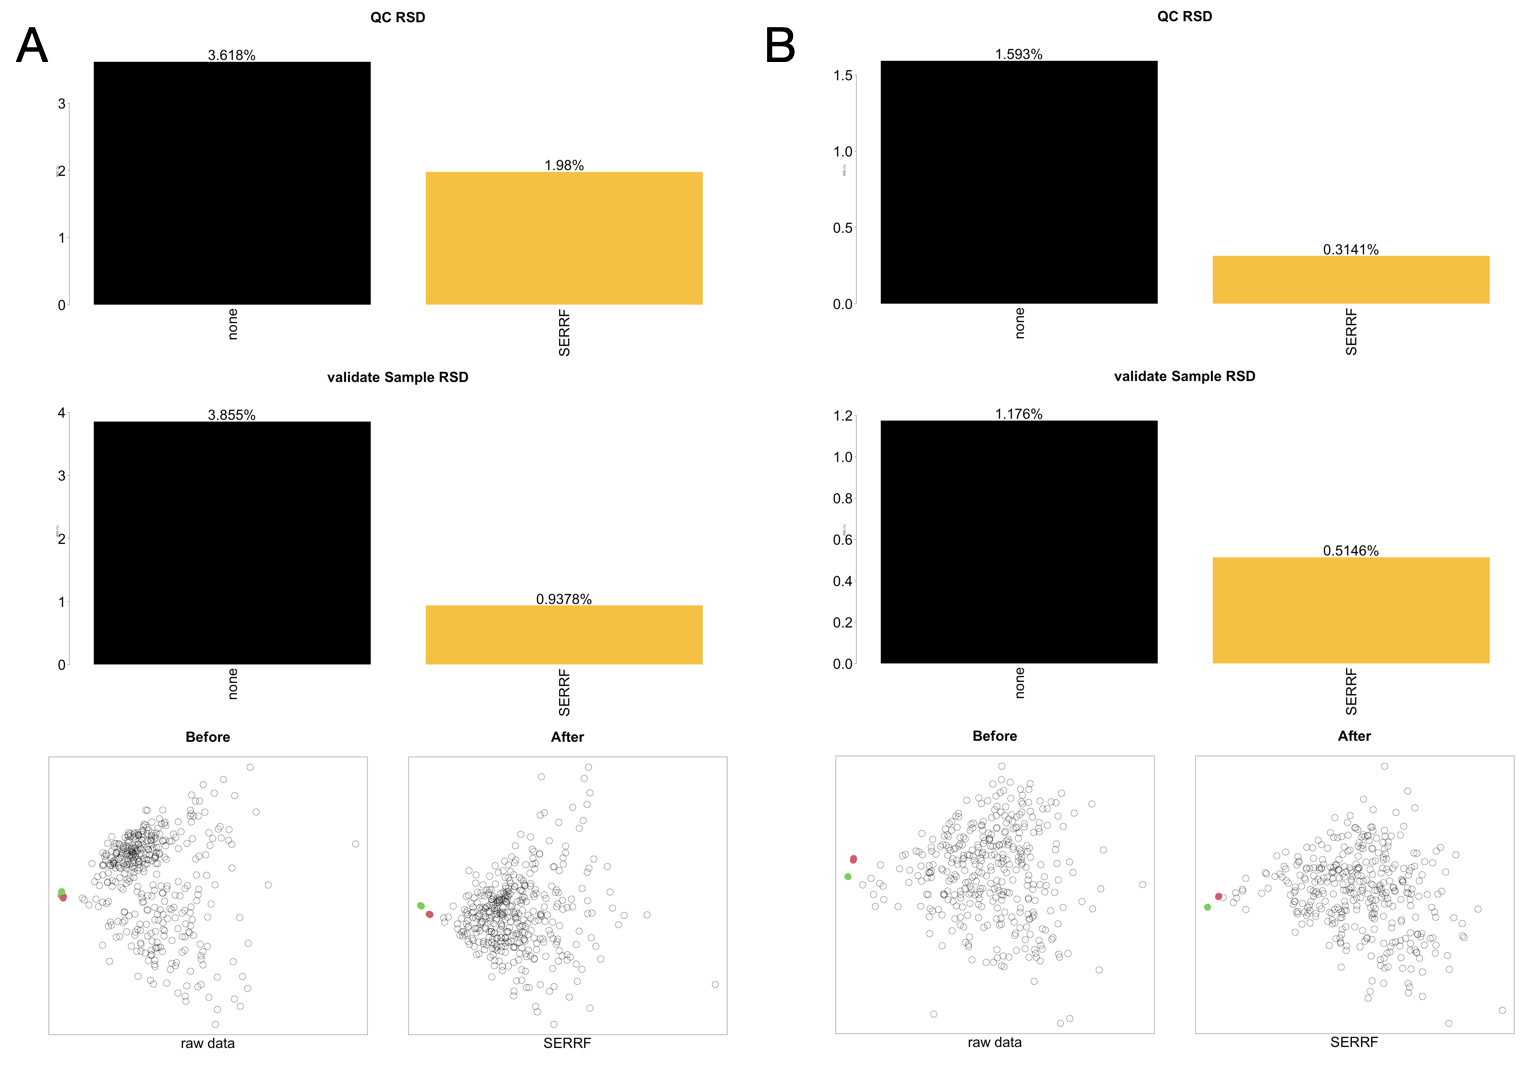
\includegraphics[width=\textwidth]{fig/supp/SuppFig2.png}
  \caption{
    SERRF-normalized quality metrics across injections. 
    {\bf(A)} Control samples: per-feature RSD distributions (boxplot) and PCA of QC vs.\ biological samples. 
    {\bf(B)} Low-Input samples: same metrics after SERRF correction. 
    Red and green dots represents blank and QC respectively. Both panels demonstrate tight RSDs and clear separation of QC from biological samples in PC1/PC2.
  }
  \label{fig:S2}
\end{figure}








%========================================================
%  Supplementary Figure 3: Spatial Analysis 
%========================================================
\begin{figure}[htp]
  \centering
  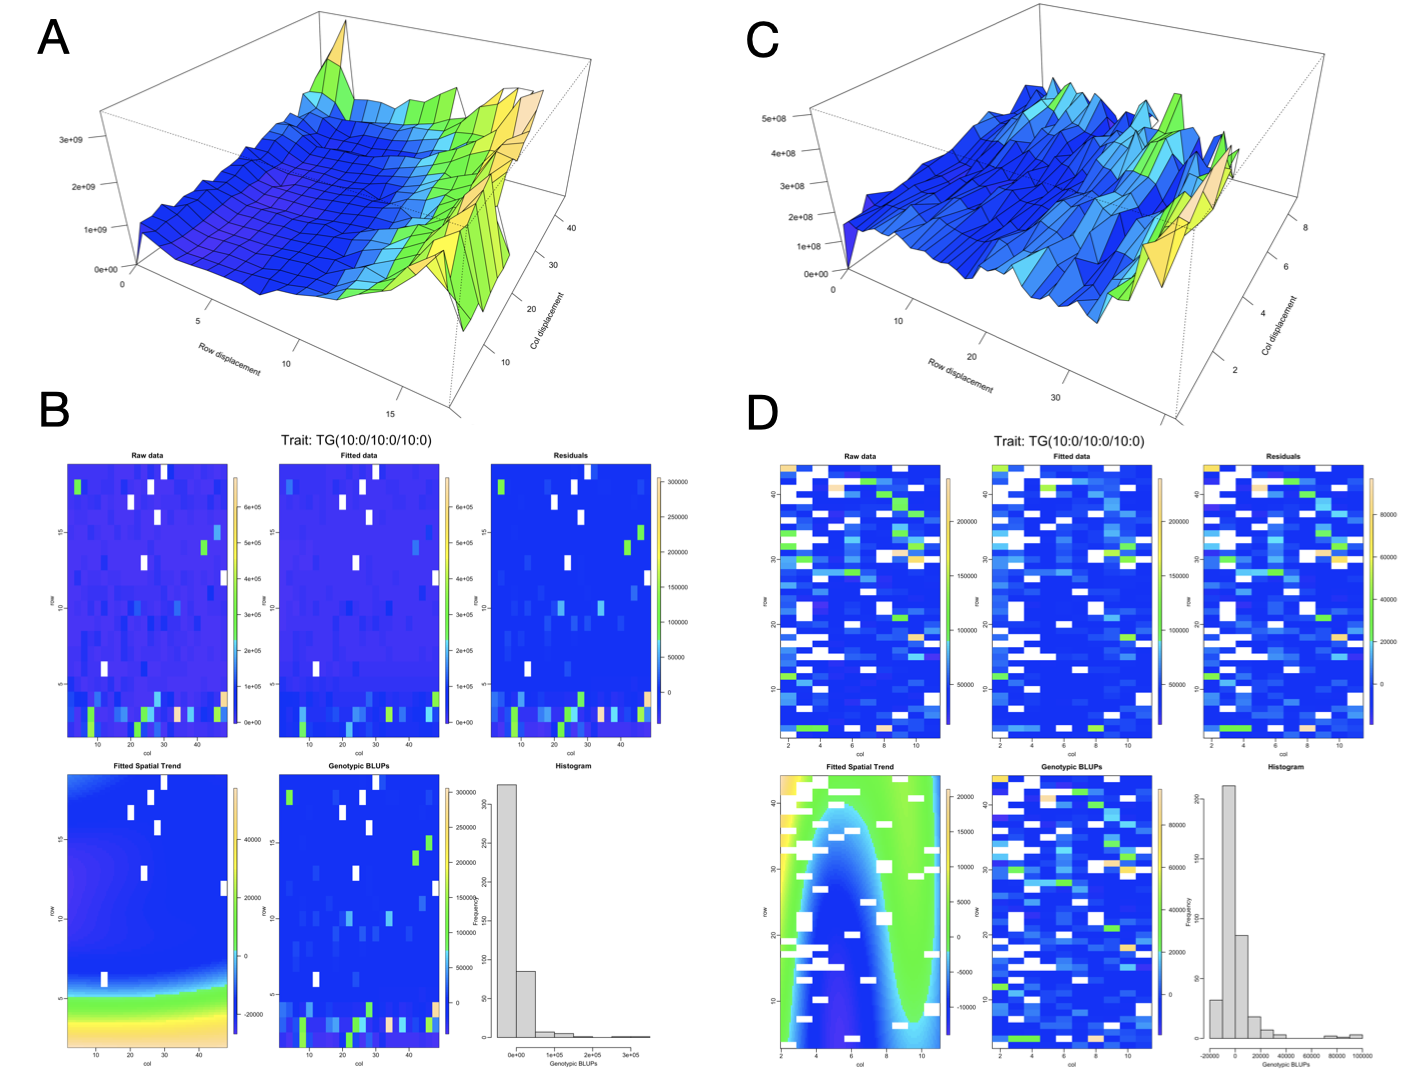
\includegraphics[width=\textwidth]{fig/supp/SuppFig3.png}
  \caption{
    Spatial‐analysis diagnostics for the lipid TG(10:0/10:0/10:0) from the SpATS model. 
    {\bf(A)} Control: 3D spatial‐trend surface (row vs.\ column displacement). 
    {\bf(B)} Control diagnostics: (i) raw data, (ii) fitted values, (iii) residuals, (iv) fitted spatial trend, (v) genotypic BLUPs, (vi) histogram of BLUPs. 
    {\bf(C)} Low‐Input: 3D spatial‐trend surface. 
    {\bf(D)} Low‐Input diagnostics, as in (B).
  }
  \label{fig:S3}
\end{figure}





%\begin{figure}[htp]
%  \centering

  % ---------- row 1 ----------
  %\begin{subfigure}[t]{0.48\textwidth}
  %  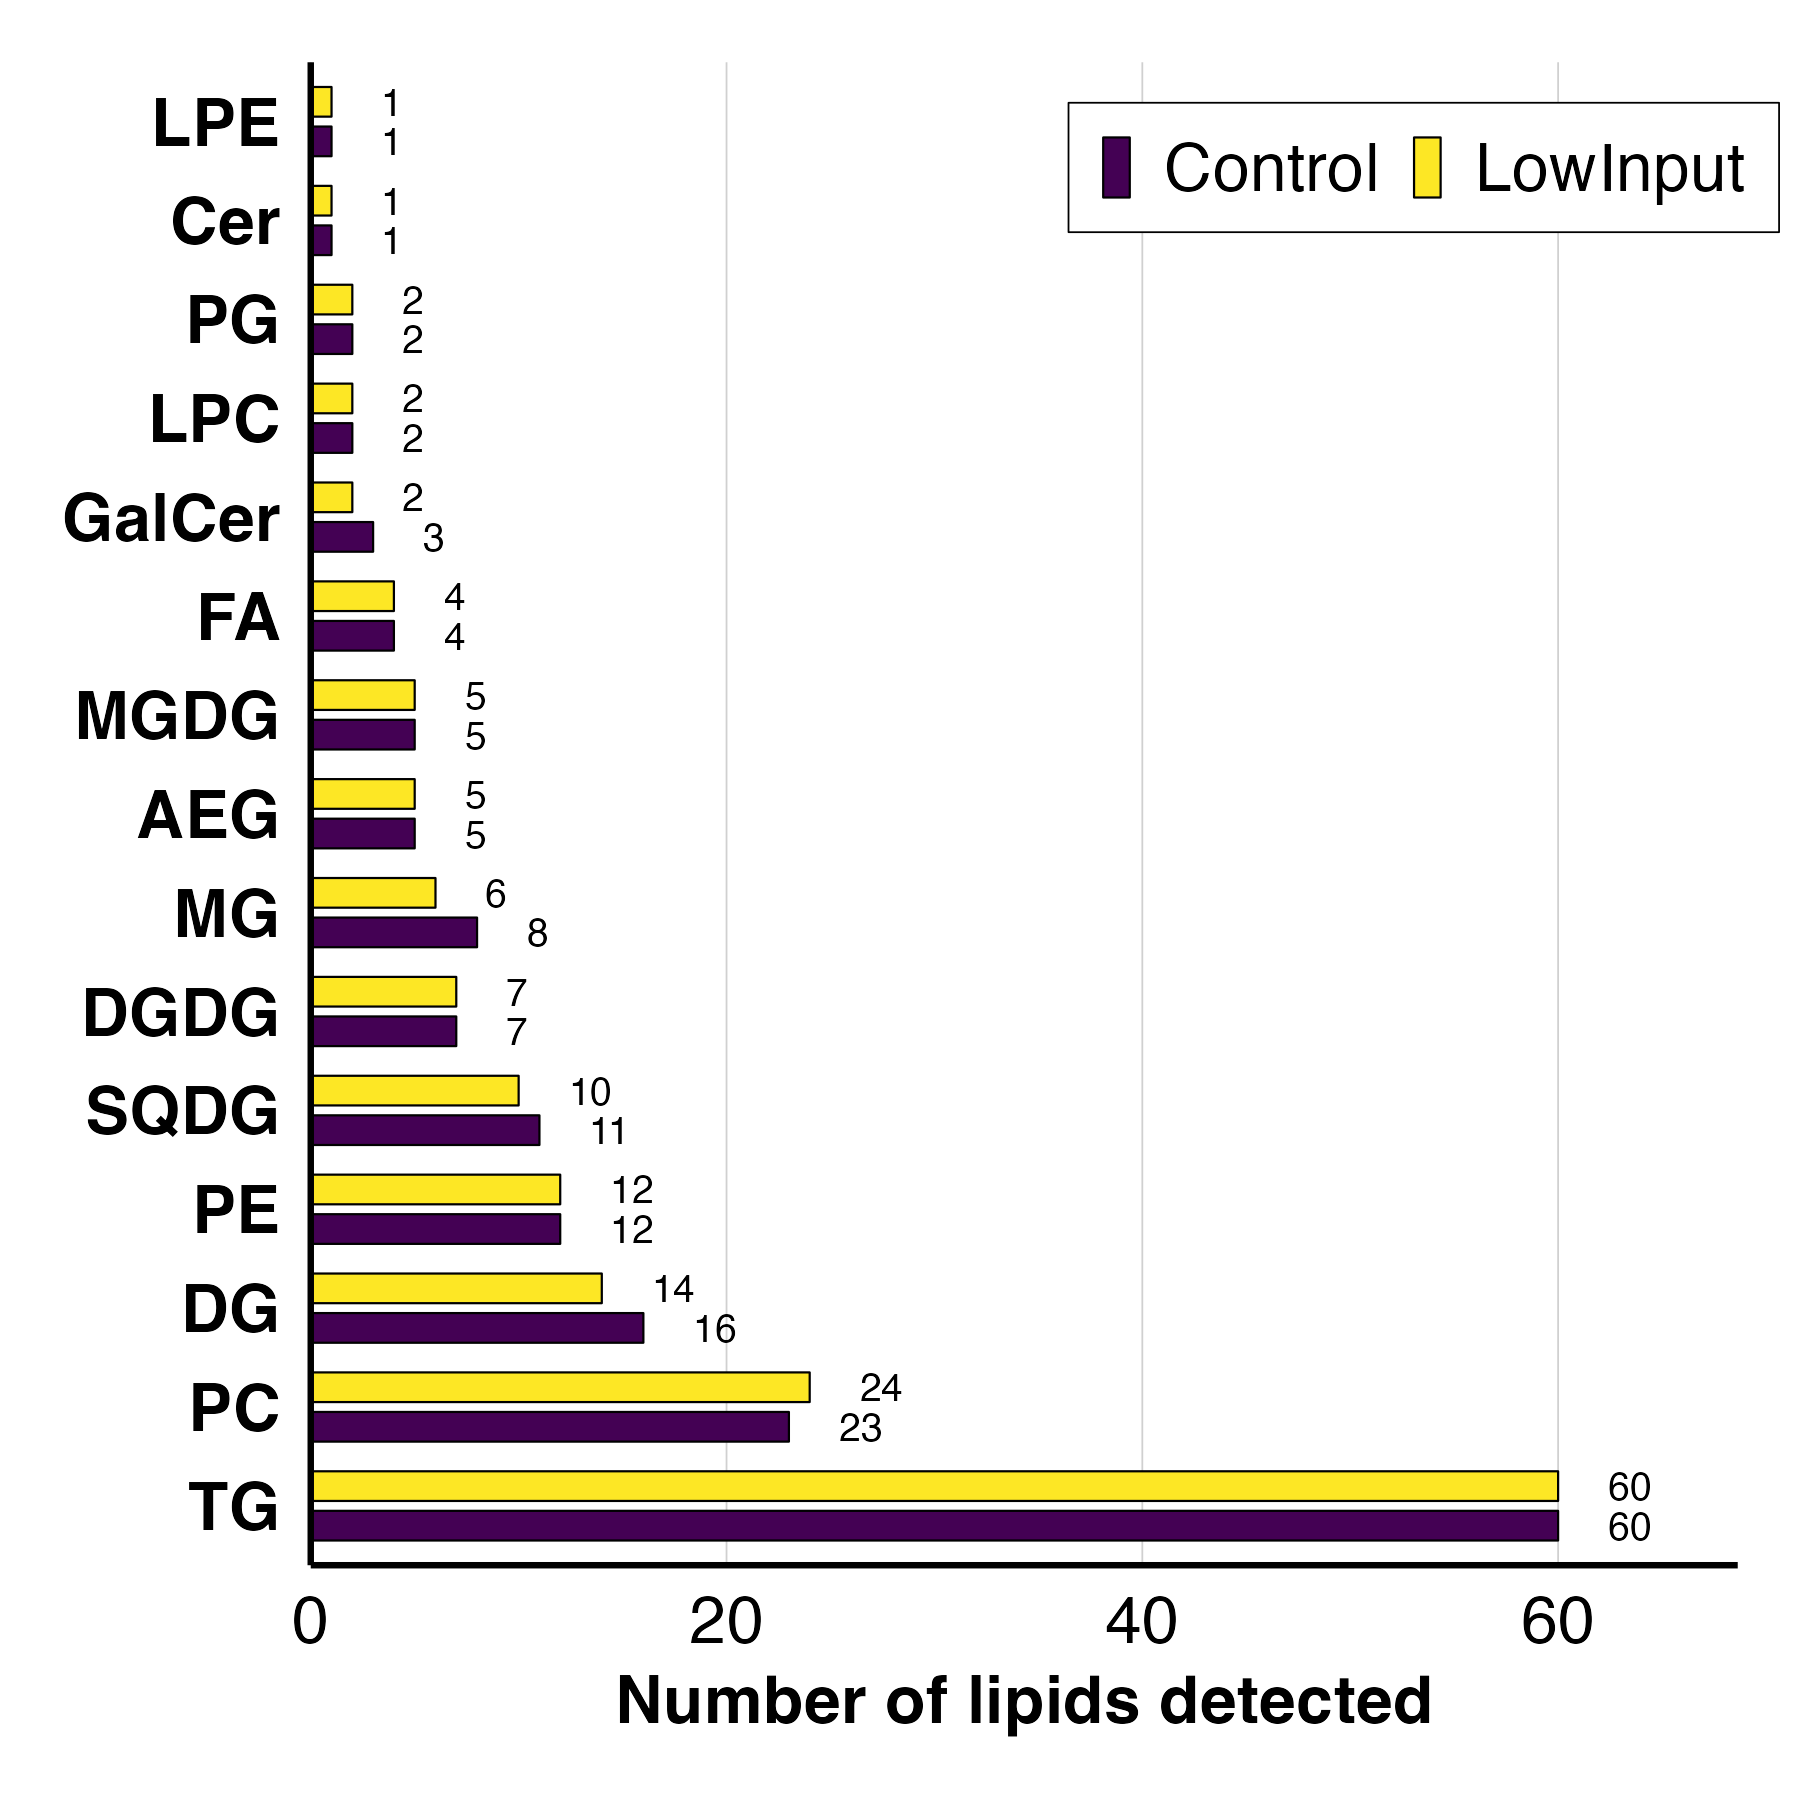
\includegraphics[width=\linewidth]{fig/supp/SuppFig_3A_Lipid_Counts.png}
  %  \caption{Number of lipid \textit{species}.}
  %  \label{fig:S3A}
  %\end{subfigure}\hfill
  %\begin{subfigure}[t]{0.48\textwidth}
  %  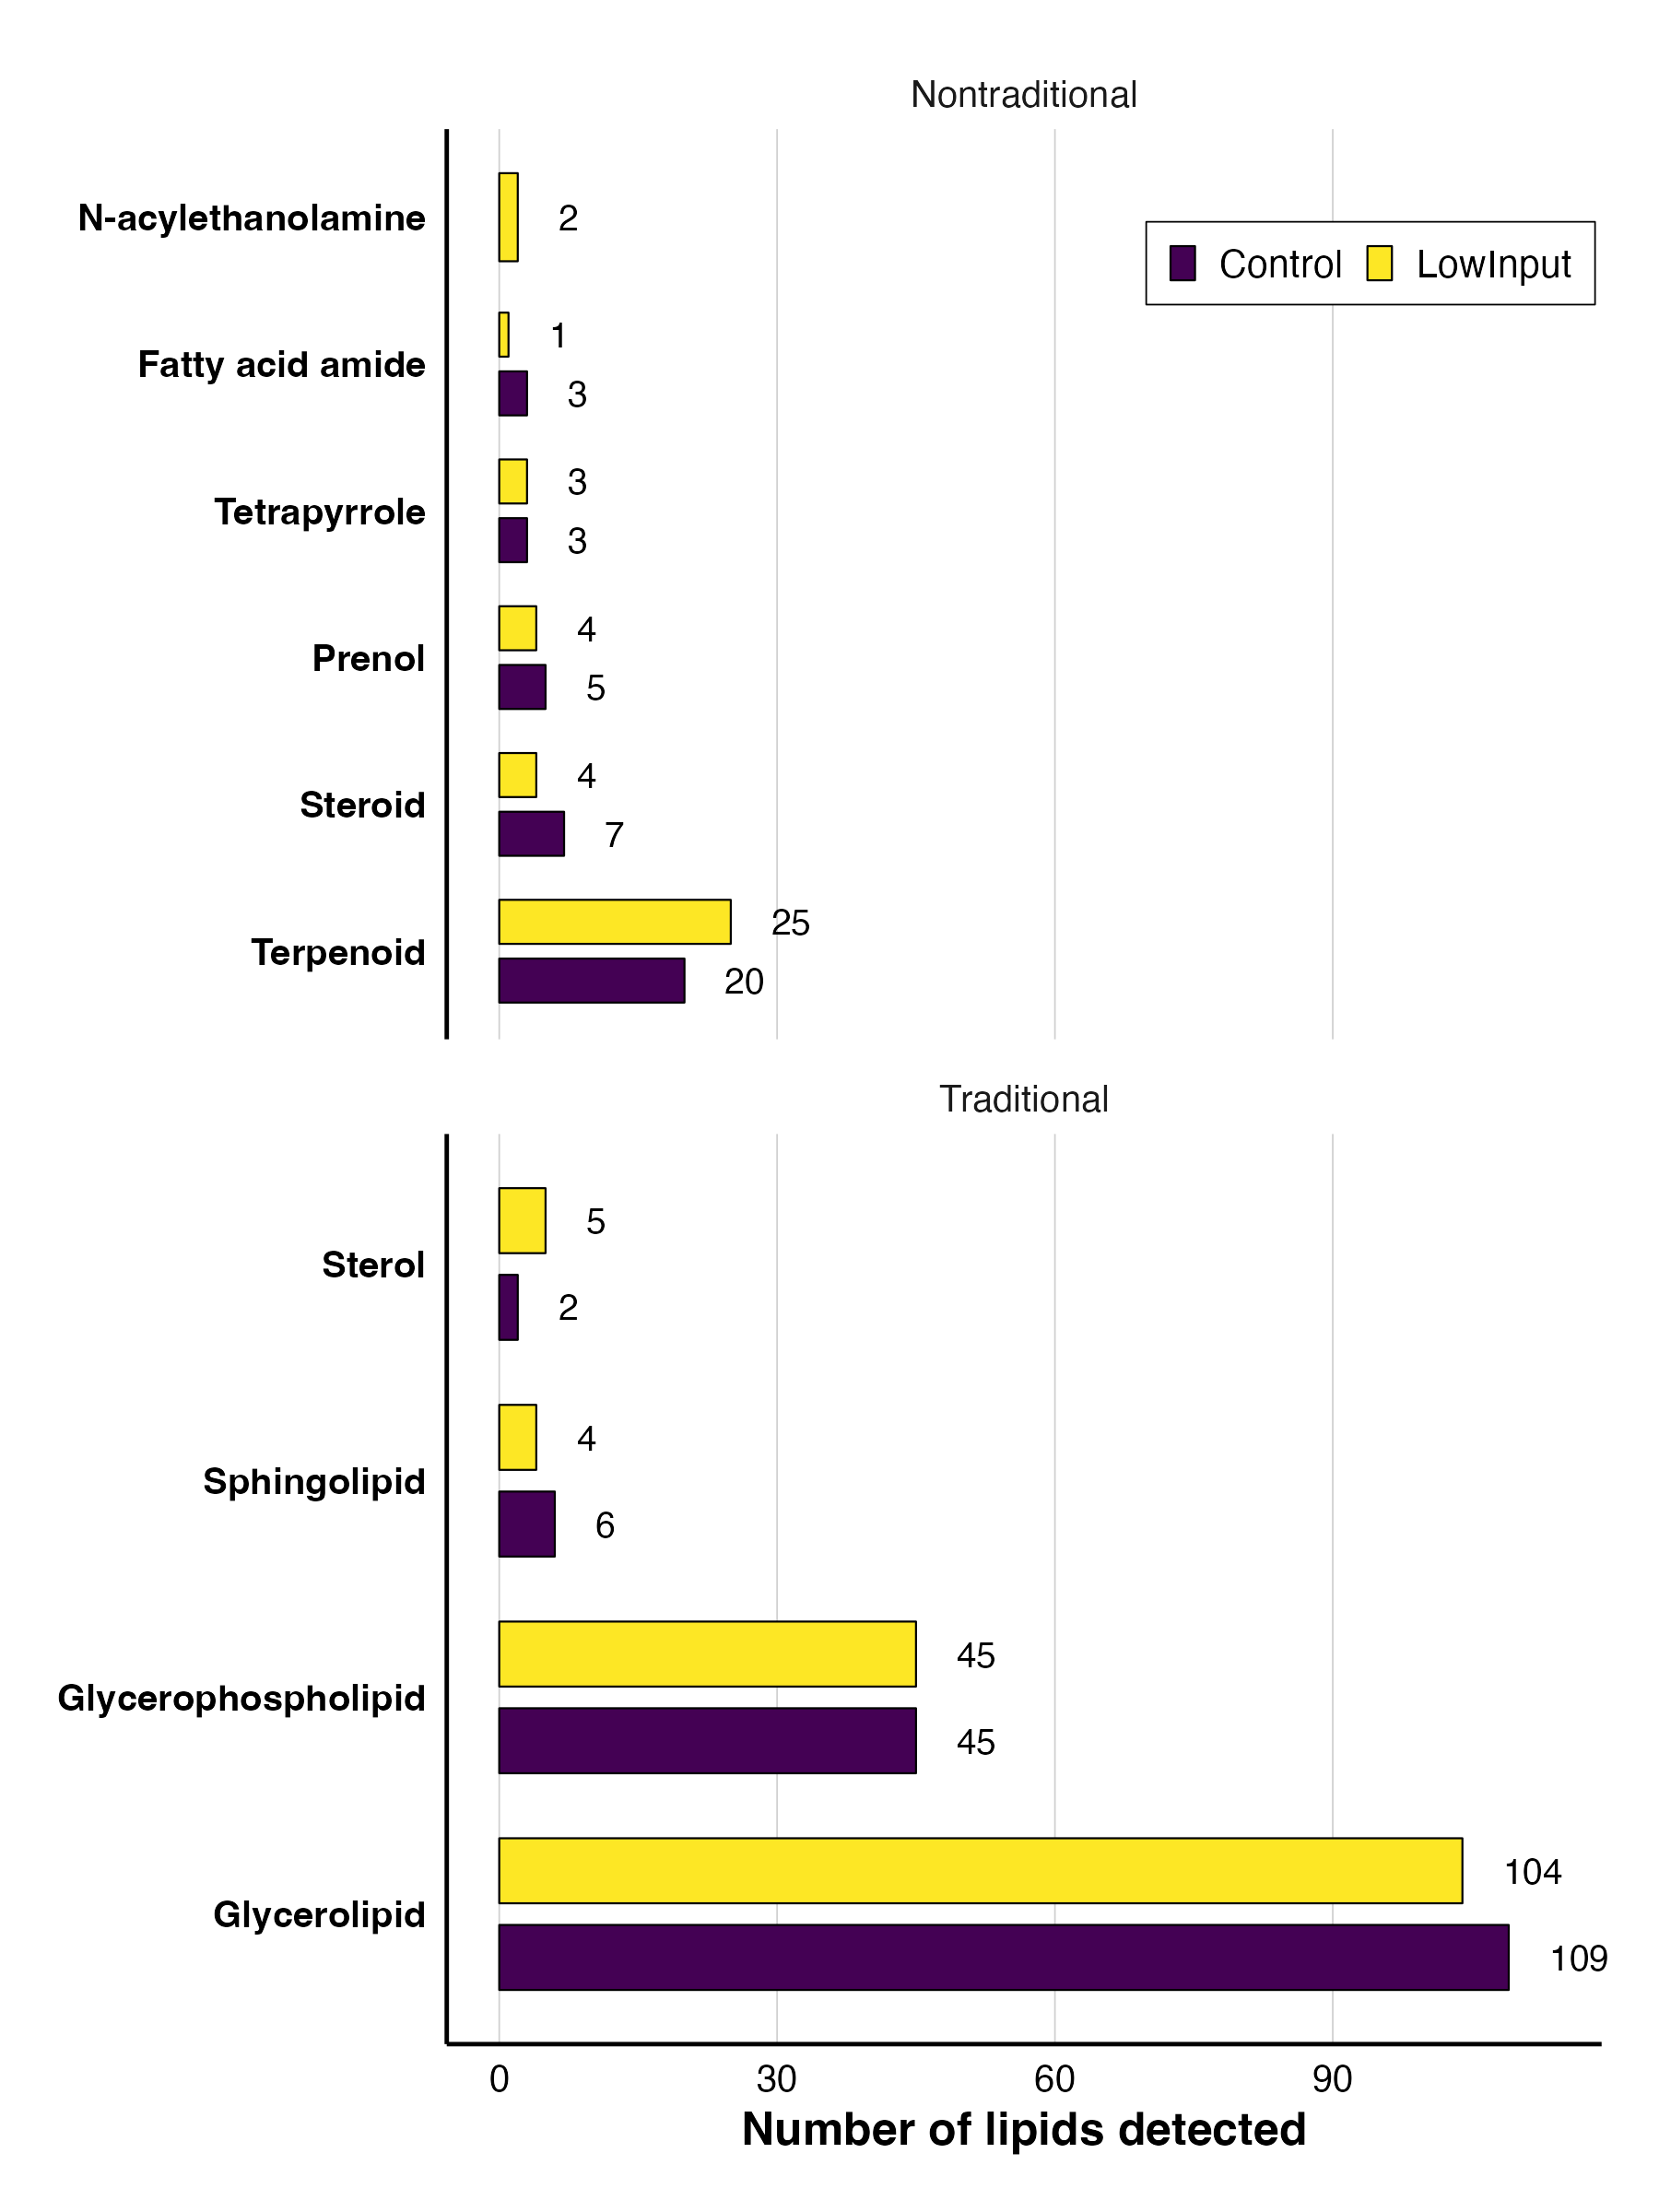
\includegraphics[width=\linewidth]{fig/supp/SuppFig_3B_trad_nontrad_counts.png}
  %  \caption{Number of lipid \textit{classes}.}
  %  \label{fig:S3B}
  %\end{subfigure}

  %\vspace{1em}

  % ---------- row 2 (centred) ----------
  %\begin{subfigure}[t]{0.55\textwidth}
  %  \centering
  %  \includegraphics[width=\linewidth]%{fig/supp/SuppFig_3C_Lipid_Overlap_Venn_traditional.png}
    %\caption{Shared and unique lipid species.}
    %\label{fig:S3C}
  %\end{subfigure}

  %\caption{Overview of lipid coverage in Control and Low-Input samples.}
  %\label{fig:S3}
%\end{figure}



%========================================================
% Supplementary Figure S4 - Lipid species/class count   (panels A, B, C, and D)
%========================================================
\begin{figure}[htp]
  \centering
  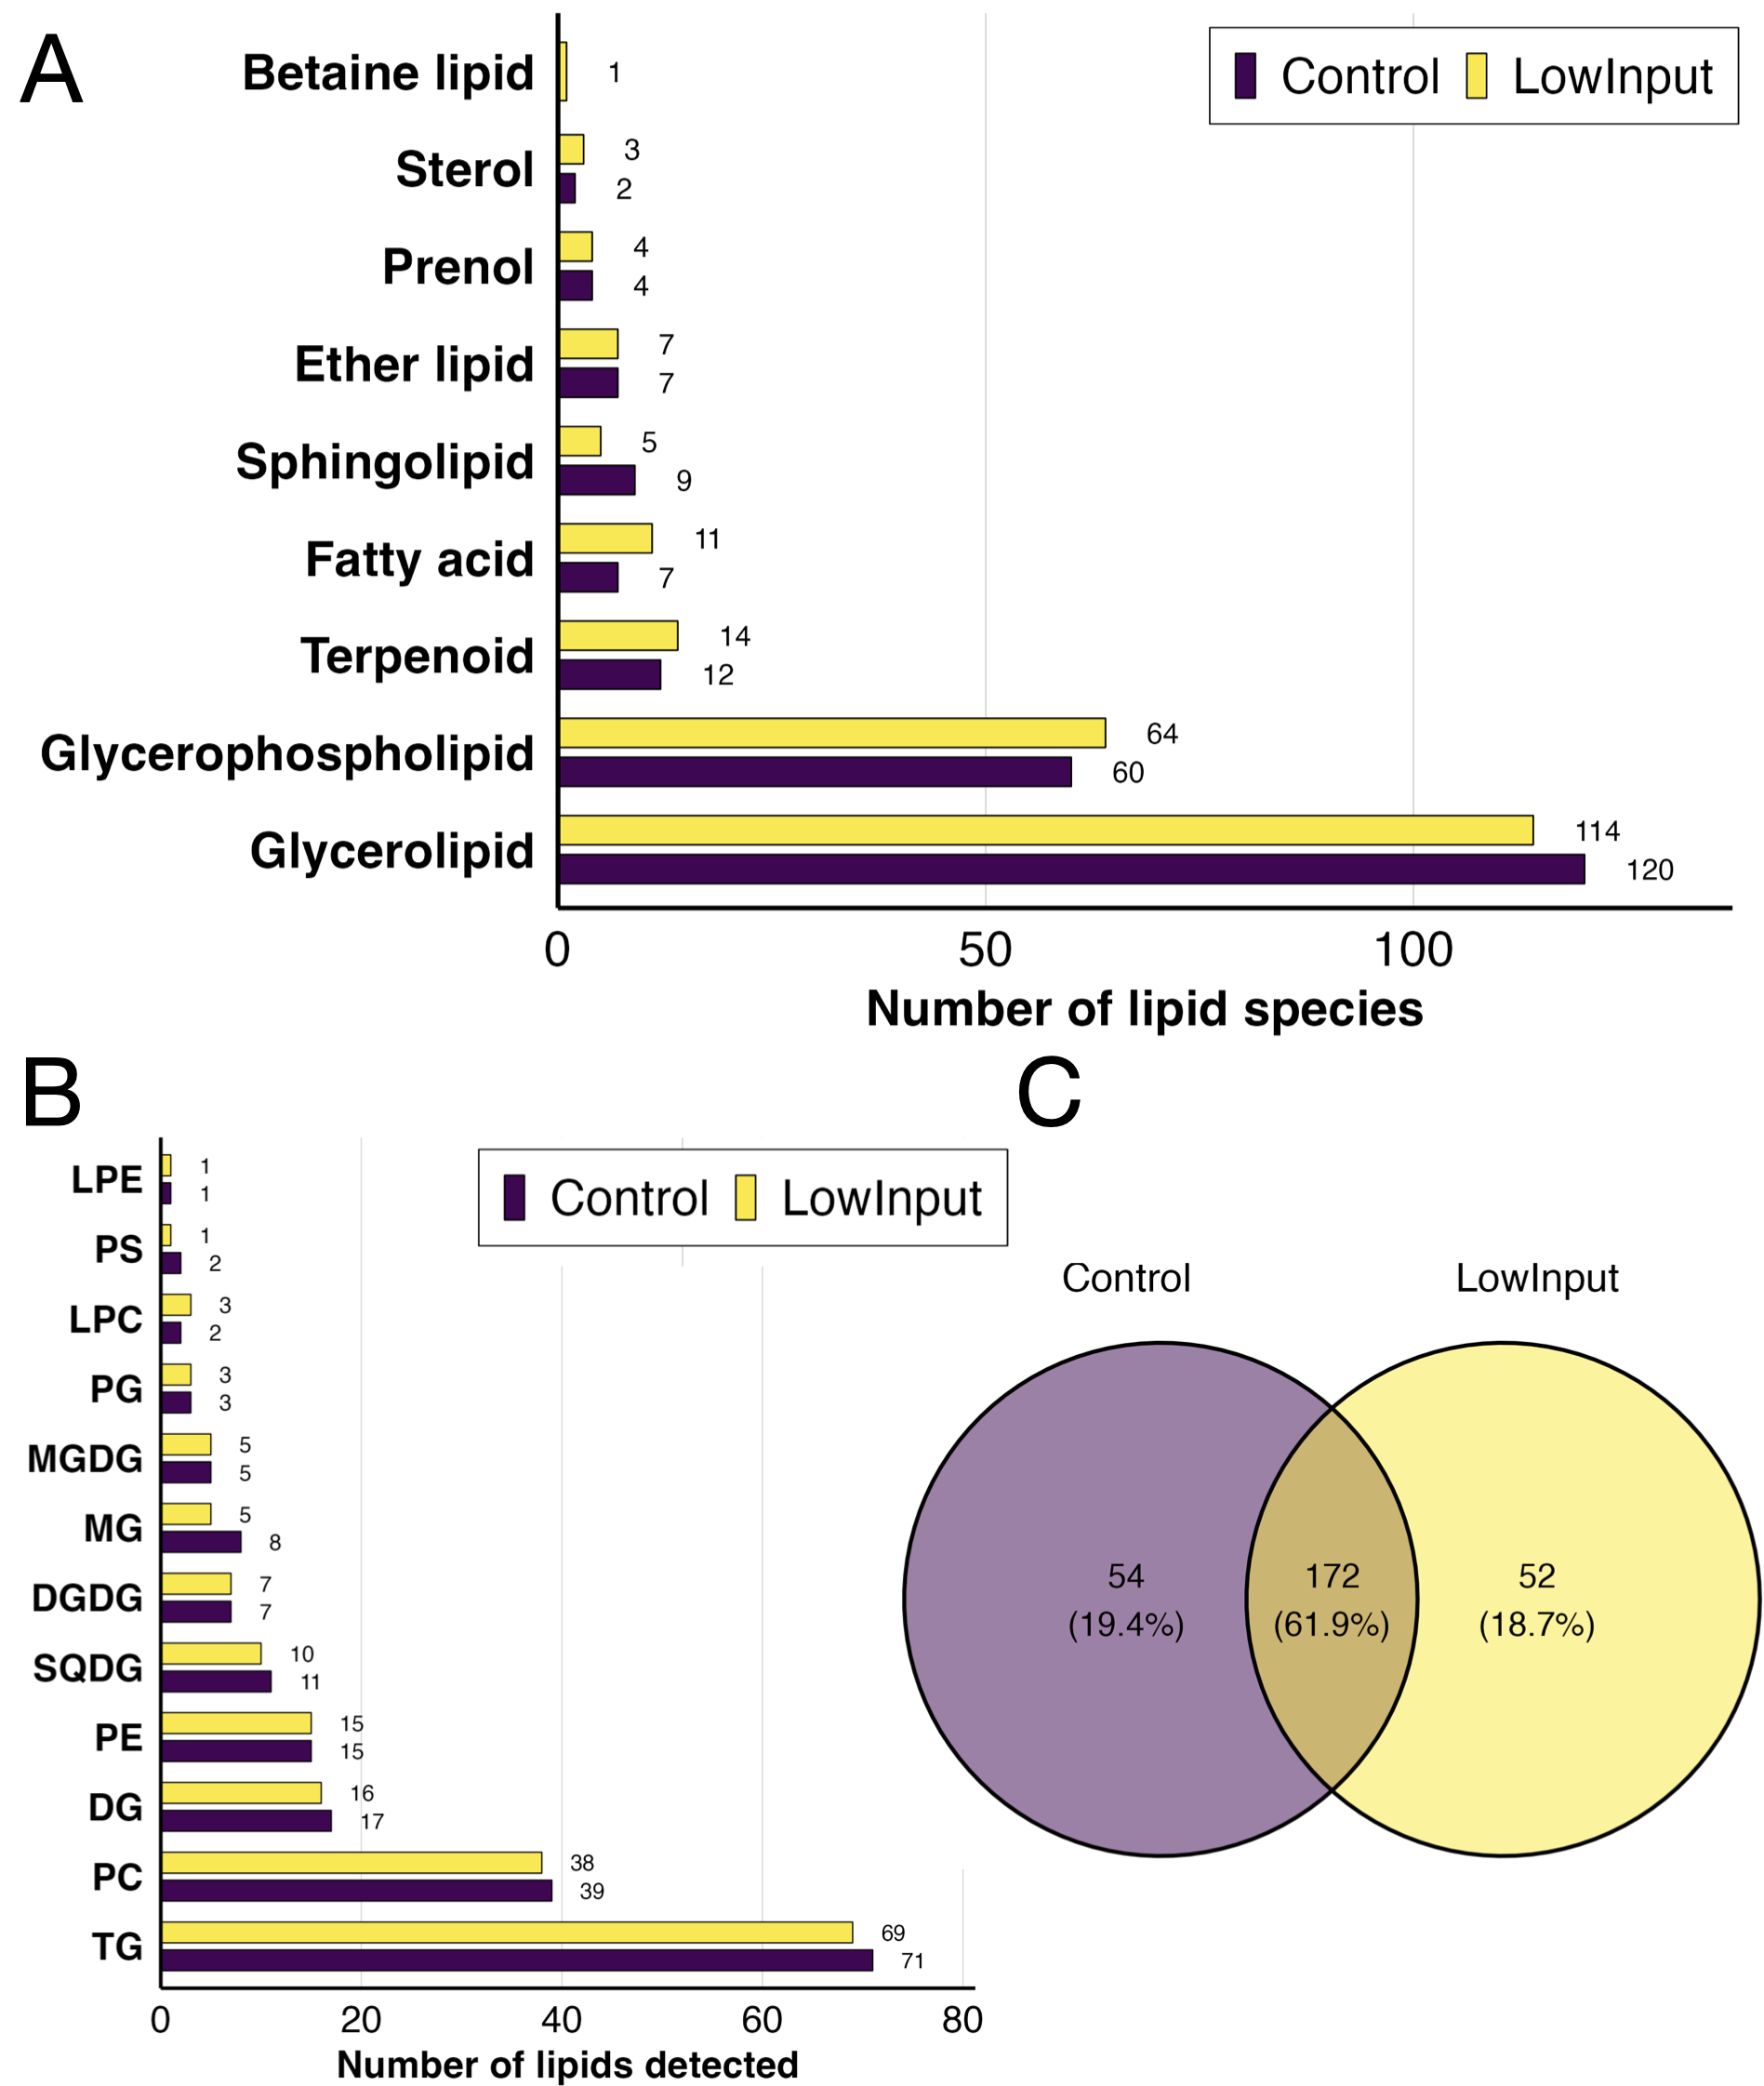
\includegraphics[width=\textwidth]{fig/supp/SuppFig4.png}
  \caption{
    Summary of lipid coverage in Control vs.\ Lowinput runs. 
    {\bf(A)} Number of detected lipid species per major class.
    {\bf(B)} Breakdown of species counts within the two largest classes: Glycerolipid and Glyverophospholipid.
    {\bf(C)} Venn diagram of all lipid species: 184 species (∼58.2\%) are shared, while Control only (65, 20.6\%) and Lowiput only (67, 21.2\%) show a small number of unique detections in each run.
  }
  \label{fig:S4}
\end{figure}


%========================================================
% Supplementary Figure S5 - TIC - Class, Glycerolipid, Glycerophospholipid
%========================================================
\begin{figure}[htp]
  \centering
  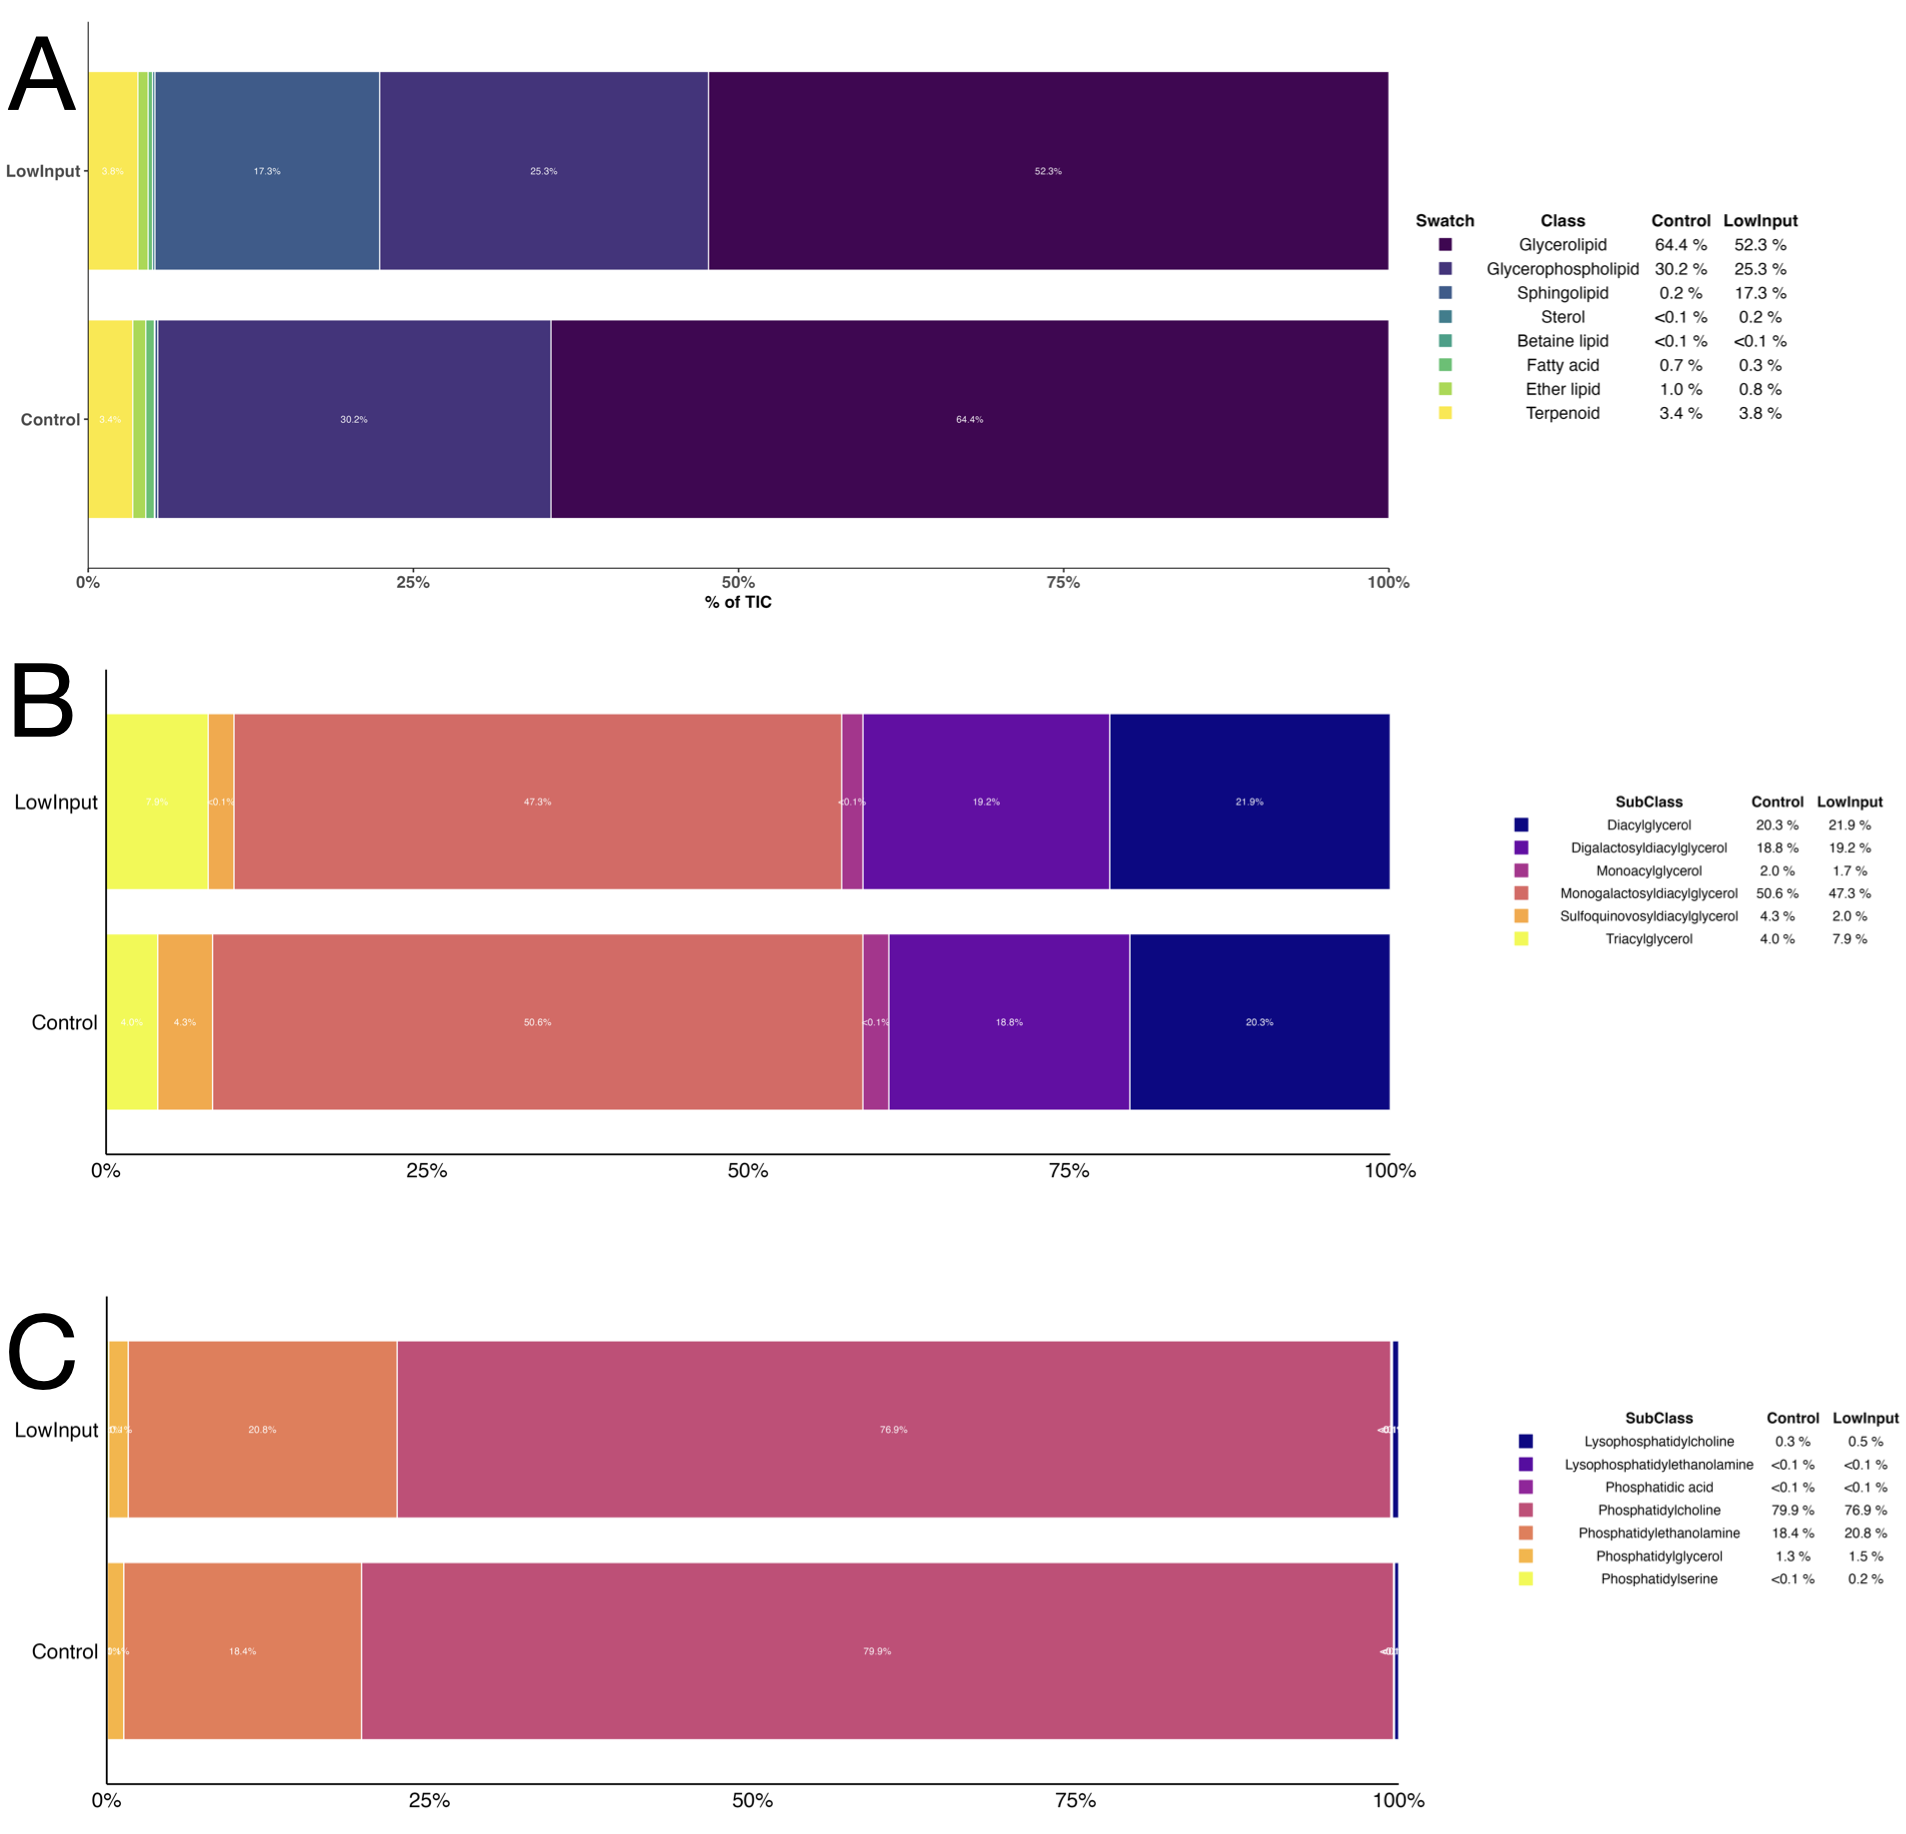
\includegraphics[width=\textwidth]{fig/supp/SuppFig5.png}
  \caption{
    Distribution of total ion current (TIC) by lipid category in Control vs.\ Lowinput samples. 
    {\bf(A)} Major lipid classes as \% of TIC: glycerolipids dominate (~64 \% Control, ~52 \% Lowinput), followed by glycerophospholipids (~30 \% vs 25 \%). Sphingolipids sees the highest change.
    {\bf(B)} Breakdown of the glycerolipid pool: mono- and di-galactosyldiacylglycerols, diacylglycerols and triacylglycerols together account for most of the glycerolipid TIC, with nearly identical subclass proportions in both runs. 
    {\bf(C)} Breakdown of the glycerophospholipid pool: phosphatidylcholines (>79 \%), phosphatidylethanolamines (~18 \%), and minor head-groups (LPC, PS, etc.) together explain the glycerophospholipid TIC. The results are very consistent between Control and Lowinput.
  }
  \label{fig:S5}
\end{figure}



%========================================================
%  Supplementary Figure S4 - Lipid ratio contrasts under low-P
%========================================================
\begin{figure}[htp]
  \centering
  % Adjust width fraction as needed (e.g., 0.8\textwidth or \textwidth)
  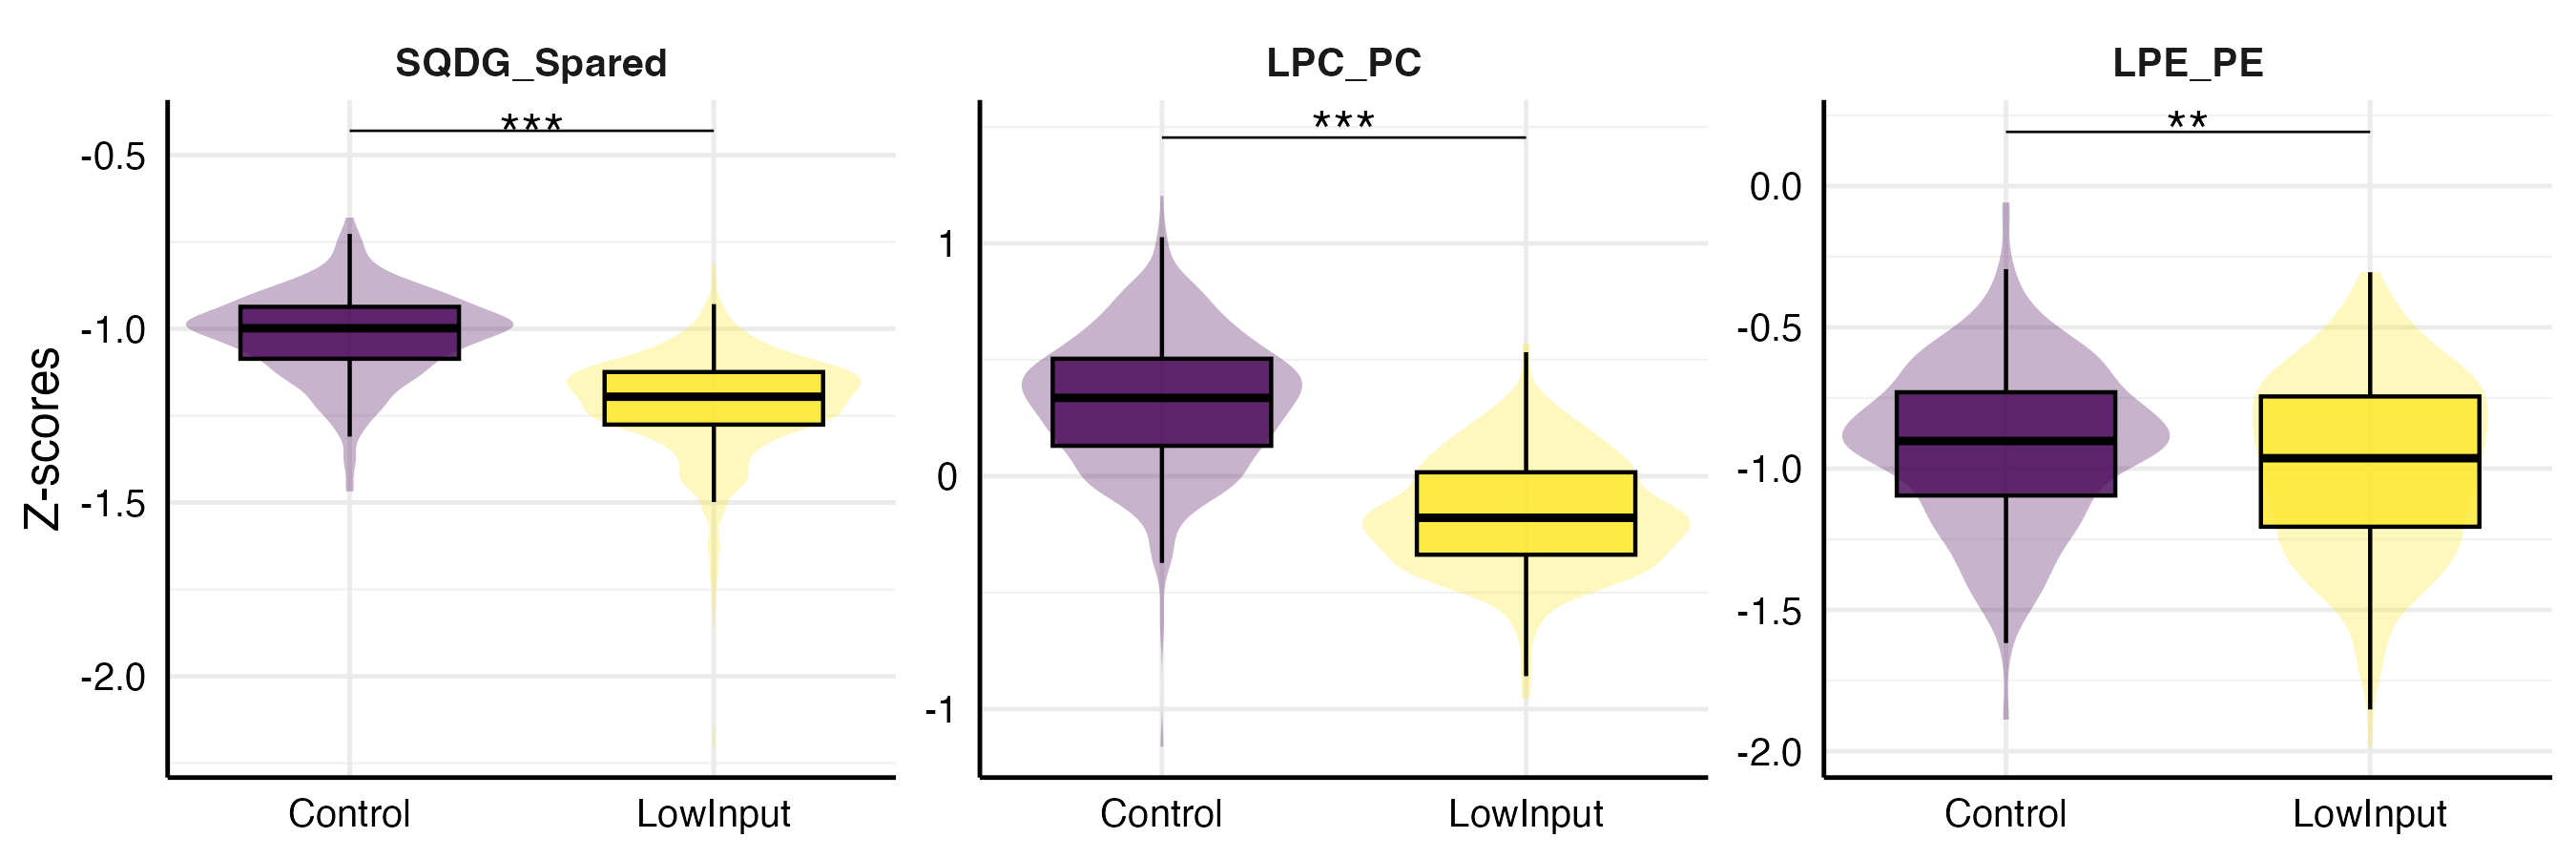
\includegraphics[width=0.8\textwidth]{fig/supp/SuppFig_4_lipid_ratio_linear_lowP.png}
  \caption{$\Delta$Z-score contrasts for lipids under LI. 
    The panel shows violin+boxplots for metrics such as \textitt{SQDG-Spared}, \textitt{LPC-PC}, and \textitt{LPE-PE} under Control versus LowInput conditions. 
    Stars denote significance levels (***: $p<0.001$, **: $p<0.01$, *: $p<0.05$) from appropriate statistical tests. 
    A negative $\Delta$Z in SQDG\_Spared indicates sulfolipid is not upregulated relative to galactolipids and PG; 
    \textitt{LPC-PC} is not significantly changed, whereas \textitt{LPE-PE} and composite Lyso\_activity shift toward values consistent with selective PE deacylation.}
  \label{fig:S4_lipid_ratio_lowP}
\end{figure}

%========================================================
%  Supplementary Figure S5 - TIC Proportions for LPC and LPE
%========================================================
\begin{figure}[htp]
  \centering
  % Adjust width fraction as appropriate, e.g., 0.6\textwidth or \textwidth
  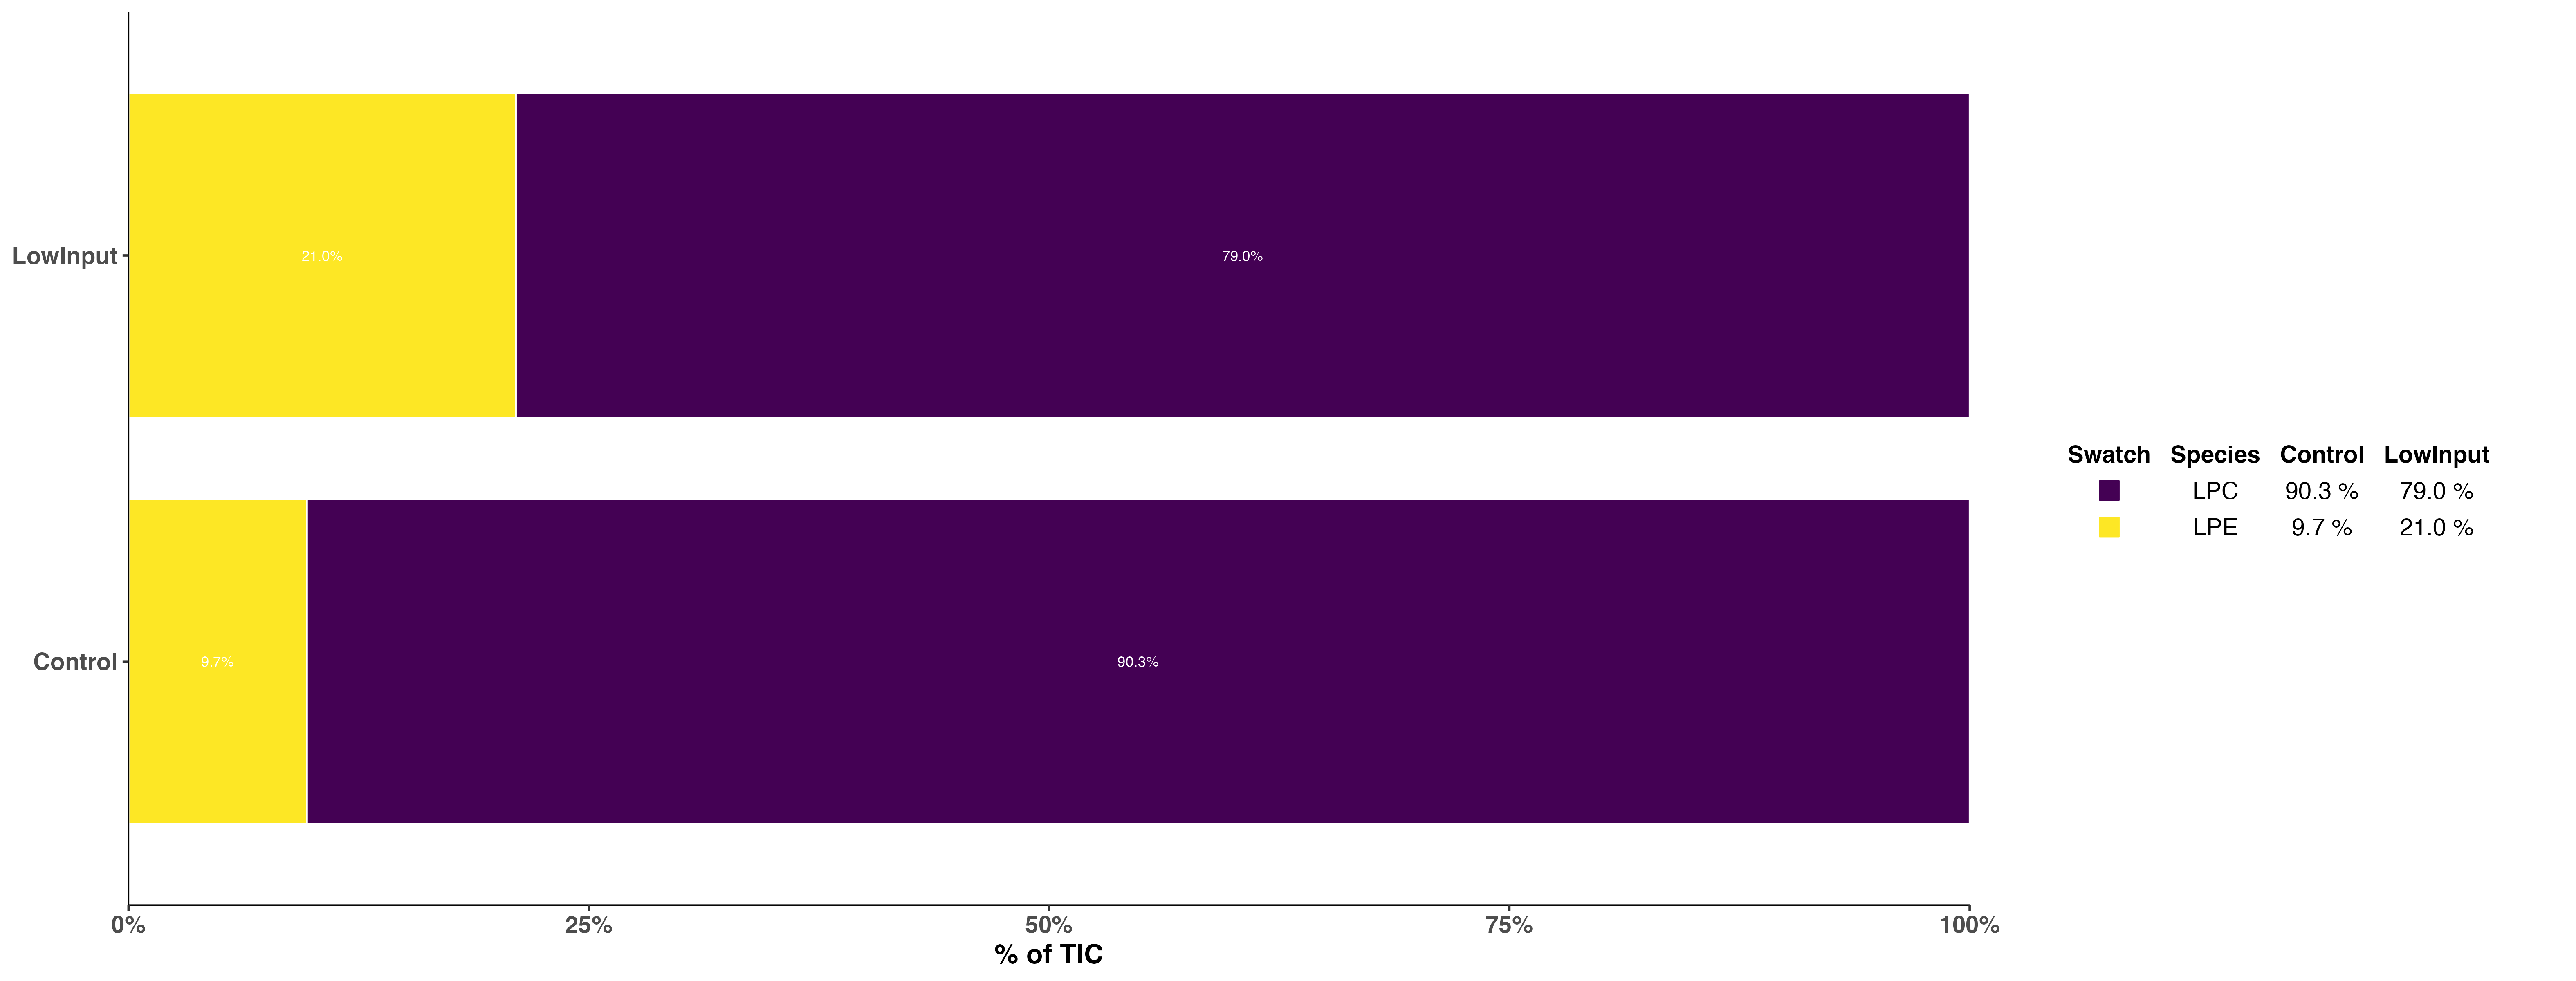
\includegraphics[width=0.7\textwidth]{fig/supp/SuppFig_5_TIC_LPC_LPE.png}
  \caption{Total ion current (TIC) proportions of lysophosphatidylcholine (LPC) and lysophosphatidylethanolamine (LPE) under Control and Low-P conditions. The plot displays relative TIC share of LPC versus LPE; stars denote significance levels (e.g., *: $p<0.05$, **: $p<0.01$) from appropriate tests. An increase in the LPE fraction and corresponding decrease in LPC under low-P suggests selective deacylation of PE for P salvage, while PC-derived LPC remains relatively stable.}
  \label{fig:S5_TIC_LPC_LPE}
\end{figure}



\end{document}


